\documentclass[11pt,  english, makeidx, a4paper, titlepage, oneside]{book}

% Packages
\usepackage{graphicx} % Usato per \includegraphics 
\usepackage{titlesec} % Usato per modificare/rimuovere le scritte Capitolo 1,2 ecc
\usepackage{textcomp} % Usaato per caratteri speciali
\usepackage{listings} % Usato per VHDL
\usepackage{xcolor} % Usato per i colori
\usepackage{amsmath}	% usato per visualizzare e avere comandi sulle equazioni
\usepackage{amssymb} % usato per simboli speciali
\usepackage{booktabs} % usato per gestire le tabelle, multicolonne
\usepackage{chngcntr} 
\counterwithin{figure}{chapter}
%\usepackage[sfdefault]{Roboto}
%\usepackage[T1]{fontenc}

% Impostazioni pagina
\textwidth 16cm % larghezza del testo nella pagina
\textheight 23cm % altezza del testo nella pagina
\topmargin -1cm % spazio in più o in meno dall'alto
\oddsidemargin 0cm % si può spostare il margine dove inizia il testo nella pagina 
\titleformat{\chapter}[display]
{\normalfont\bfseries}{}{0pt}{\Huge} % Rimuove le scritte Capitolo 1,2 ecc
\newenvironment{listato}{\footnotesize} {\normalsize }
\renewcommand{\arraystretch}{1.4} % modifica altezza delle celle in tabella


% inizio del documento
\begin{document}

% pagina iniziale
\begin{titlepage}

	\centerline{
\includegraphics[width=3cm]{./img/general/polito.png}}
	\vspace{0.3cm}
	\centerline{\Large{Politecnico di Torino}}
	\vspace{0.3cm}
	\centerline{\Large{III Facoltà di Ingegneria}}
	\vspace{3cm}
	\centerline{\Huge\textbf{Sistemi elettronici a basso consumo}}
	\vspace{1cm}
	\centerline{\LARGE\textbf{Relazioni di laboratorio}}
	\vspace{3cm}
	\centerline{\LARGE{Laurea Magistrale in Ingegneria Elettronica}}
	\vspace{0.3cm}
	\centerline{\LARGE{Orientamento: Sistemi Elettronici}}
	\vspace{3cm}
	\centerline{\Large{Gruppo n. 9}}
	\vspace{2cm}
	\centerline{\Large{Autori:}}
	\vspace{0.3cm}
	\centerline{\Large{Favero Simone, Micelli Federico, Spanna Francesca}}
	
\end{titlepage}

\tableofcontents % imposta l'indice in automatico
\pagebreak % per passare direttamente alla prossima pagina

\chapter{Stima di potenza mediante tecniche probabilistiche}

\section{Calcolo di probabilità e attività: porte logiche elementari}

Il primo esercizio consiste nel valutare probabilità e attività dell'uscita di 
quattro porte logiche elementari: NOT, AND, OR e XOR.
\\\\
\centerline{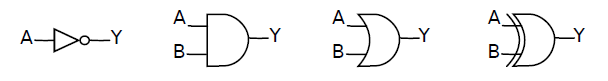
\includegraphics[width=12cm]{./img/Lab_1/Es_1/Porte.png}}
\\\\
Mentre la probabilità dell'uscita del gate è definita dalla funzione logica
stessa, la switching activity è valutata allo stesso modo per tutti i casi, 
mediante la seguente formula:
\\\\
	\centerline{$A = 2 \cdot P1 \cdot (1-P1)$}
\\\\
dove $P1$ indica la probabilità che l'uscita assuma valore logico alto.\\\\
Di seguito è riportata l'analisi delle porte logiche richieste, considerando 
ingressi equiprobabili e scorrelati.

\begin{itemize}
	\item \textbf{NOT} \\
	$P(Y=1) = 1 - P(A=1) = 0.5$ \\
	$A(Y) = 0.5$
	\item \textbf{AND} \\
	$P(Y=1) = P(A=1) \cdot P(B=1) = 0.25$ \\
	$A(Y) = 0.375$
	\item \textbf{OR} \\
	$P(Y=1) = 1-((1-P(A=1)) \cdot(1-P(B=1))) = 0.75$ \\
	$A(Y) = 0.375$
	\item \textbf{XOR} \\
	$P(Y=1) = P(A=1) \cdot(1-P(B=1)) + P(B=1) \cdot(1-P(A=1)) = 0.5$ \\
	$A(Y) = 0.5$ 
\end{itemize} 
Attraverso una simulazione ModelSim, è possibile ottenere un file 
contenente il numero di commutazioni di ogni segnale del circuito durante il 
tempo di simulazione.
\\
Il testbench fornito sfrutta un generatore di numeri casuali per generare gli 
ingressi delle porte, rendendo questi ultimi equiprobabili e statisticamente 
indipendenti.
\\
Sono riportati i seguenti valori:
\\
\begin{center}
	\begin{tabular}{|c|c|c|c|c|} %numero di colonne
 	\hline % tira una riga
 	Tc(CK) & Tc(INV) & Tc(AND) & Tc(OR) & Tc(XOR) \\ 
 	\hline
 	20 & 1 & 0 & 4 & 4 \\ 
 	\hline
 	200 & 43 & 40 & 42 & 44 \\ 
 	\hline
 	2000 & 533 & 418 & 352 & 470 \\
 	\hline
 	20000 & 4916 & 3606 & 3784 & 4876 \\
 	\hline
 	200000 & 49967 & 37834 & 37541 & 49939 \\
 	\hline
	\end{tabular}
\end{center}
\vspace{0.3cm}
È possibile stimare la switching activity dividendo il numero 
di commutazioni di un nodo per il numero di colpi di clock della
relativa simulazione.
\\
Dal momento che il parametro Tc si riferisce al numero totale di 
commutazioni, il numero di cicli di clock è ottenuto dividendo per due
il parametro Tc(CK).
\\\\
I risultati dei calcoli sono riportati nella seguente tabella. 
\\
\begin{center}
	\begin{tabular}{|c|c|c|c|c|}
	\hline
	Tc(CK) & Esw(INV) & Esw(AND) & Esw(OR) & Esw(XOR) \\ 
	\hline
	20 & 0.1 & 0 & 0.4 & 0.4 \\
	\hline
	200 & 0.43 & 0.40 & 0.42 & 0.44 \\
	\hline
	2000 & 0.533 & 0.418 & 0.352 & 0.470 \\
	\hline
	20000 & 0.4916 & 0.3606 & 0.3784 & 0.4876 \\
	\hline
	200000 & 0.4997 & 0.3783 & 0.3754 & 0.4994 \\
	\hline
	\end{tabular}
\end{center}
\vspace{1cm}
Per garantire una migliore visualizzazione dei dati ottenuti 
al variare del tempo di simulazione, sono stati realizzati 
i seguenti grafici.
\\\\
\centerline{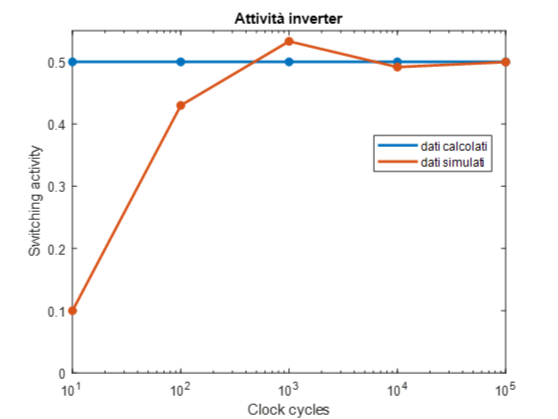
\includegraphics[width=8cm]{./img/Lab_1/Es_1/Inverter.png}
            \includegraphics[width=8cm]{./img/Lab_1/Es_1/AND.png}}
\centerline{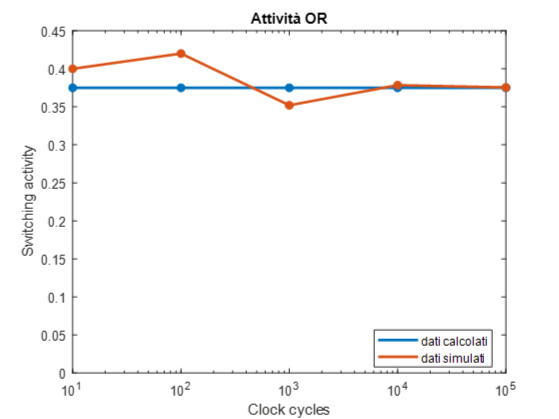
\includegraphics[width=8cm]{./img/Lab_1/Es_1/OR.png}
            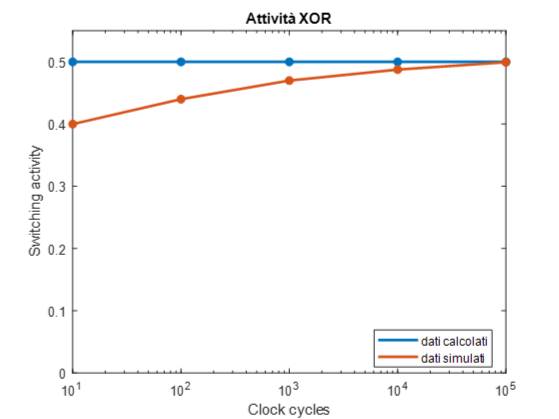
\includegraphics[width=8cm]{./img/Lab_1/Es_1/XOR.png}}
\\\\
Si osserva che, all'aumentare del tempo di simulazione, la stima 
dell'attività risulta sempre più accurata. In particolare, 
nel caso analizzato, si osserva che per un numero di cicli di clock 
superiore a 10000, i dati simulati sono confrontabili con quelli teorici.
\newpage

\section{Calcolo di probabilità e attività: half adder e full adder} 
Dalle tavole di verità di Half Adder e Full Adder si ottengono le seguenti funzioni:
\begin{itemize}
	\item \textbf{Half adder} \\
	\centerline{S = A XOR B} \\
	\centerline{Cout = A AND B}
	\item \textbf{Full adder} \\
	\centerline{S = A XOR B XOR Cin} \\
	\centerline{Cout = (A AND B) OR (A AND Cin) OR (B AND Cin)}\\
\end{itemize}
Partendo dalle funzioni logiche che descrivono le uscite è stato possibile ricavare le probabilità
associate ad esse e le relative attività.
\begin{itemize}
	\item \textbf{Half adder}\\
	\begin{align*}
	P(S=1) &= P(A=1) \cdot ((1-P(B=1)) + P(B=1) \cdot (1-P(A=1))\\\\
	P(Cout=1) & = P(A=1) \cdot P(B=1)\\\\
	A(S) &= 2 \cdot P(S=1) \cdot (1-P(S=1))\\\\
    A(Cout) &= 2 \cdot P(Cout=1) \cdot (1-P(Cout=1)) 
    \end{align*}	
	\item \textbf{Full adder}
	\begin{align*}
	P(S=1) & = P(A=1) \cdot(1-P(B=1)) \cdot (1-P(Cin=1)) + \\ 
	          & + P(B=1) \cdot(1-P(A=1)) \cdot (1-P(Cin=1)) + \\
	          & + P(Cin=1) \cdot (1-P(A=1)) \cdot(1-P(B=1)) + \\
	          & + P(A=1) \cdot P(B=1) \cdot P(Cin=1)\\\\
	 P(Cout=1) & = P(A=1) \cdot P(B=1) \cdot (1-P(Cin=1)) +\\
	 					& + P(Cin=1) \cdot P(A=1) \cdot (1-P(B=1)) +\\
	 					& + P(Cin=1) \cdot P(B=1) \cdot (1-P(A=1)) +\\
	 					& + P(A=1) \cdot P(B=1) \cdot P(Cin=1)\\\\
	 A(S) & = 2 \cdot P(S=1) \cdot (1-P(S=1))\\\\
	A(Cout) & = 2 \cdot P(Cout=1) \cdot (1-P(Cout=1))
	\end{align*}	
\end{itemize} 
I risultati ottenuti sono riportati nella seguente tabella.
\vspace{0.3cm}
\begin{center}
	\begin{tabular}{|c|c|c|c|c|}
	\hline
	\multicolumn{5}{|c|}{P(A) = P(B) = 0.5  }\\
	\hline
	  & P(S=1) & A(S) & P(Cout=1) & A(Cout) \\ 
	\hline
	HA & 0.5 & 0.5 & 0.25 & 0.375 \\
	\hline
	FA & 0.5 & 0.5 & 0.5 & 0.5 \\
	\hline
	\end{tabular}
\end{center}
\vspace{0.3cm}
Sfruttando i risultati ottenuti per il singolo full adder, è stato possibile ottenere le probabilità e le attività di un ripple carry adder avente parallelismo pari a 8 bit.
\\\\\\
\centerline{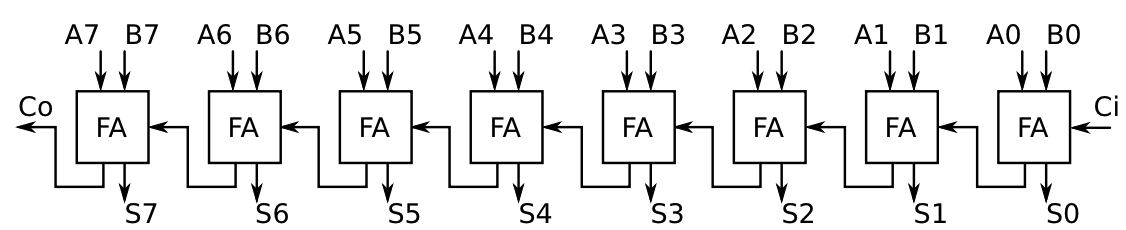
\includegraphics[width=15cm]{./img/Lab_1/Es_2/RCA_8_bit.png}}
\\\\\\
Per tale analisi sono stati considerati equiprobabili e scorrelati gli ingressi A e B mentre il carry in ingresso al primo full adder è stato fissato a 0.\\
I risultati ottenuti sono riportati nella seguente tabella.
\vspace{0.3cm}
\begin{center}
\begin{tabular}{|c|c|c|c|c|c|c|c|c|c|}
\hline
\multicolumn{10}{|c|}{P(A) = P(B) = 0.5}\\
\hline
 & S7 & S6 & S5 & S4 & S3 & S2 & S1 & S0 & Cout \\
\hline
P(Y=1) & 0.5 & 0.5 & 0.5 & 0.5 & 0.5 & 0.5 & 0.5 & 0.5 & 0.4980 \\
\hline
A(Y) & 0.5 & 0.5 & 0.5 & 0.5 & 0.5 & 0.5 & 0.5 & 0.5 & 0.5 \\
\hline
\end{tabular}
\end{center}
\vspace{0.3cm}
Variando le probabilità associate agli ingressi, in particolare considerando P(A=1) = 0.4 e P(B=1) = 0.6, si ottengono i seguenti risultati.
\vspace{0.3cm}
\begin{center}
\begin{tabular}{|c|c|c|c|c|c|c|c|c|c|}
\hline
\multicolumn{10}{|c|}{P(A) = 0.4 e P(B) = 0.6}\\
\hline
 & S7 & S6 & S5 & S4 & S3 & S2 & S1 & S0 & Cout \\
\hline
P(Y=1) & 0.52 & 0.5104 & 0.5054 & 0.5028 & 0.5015 & 0.5008 & 0.5004 & 0.5002 & 0.4973 \\
\hline
A(Y) & 0.4992 & 0.4998 & 0.4999 & 0.5 & 0.5 & 0.5 & 0.5 & 0.5 & 0.5 \\
\hline
\end{tabular}
\end{center}
\vspace{0.3cm}
È possibile notare come la probabilità delle varie uscite sia funzione delle probabilità degli ingressi.
In particolare, la probabilità delle uscite relative alle somme aumenta. Si nota che ai bit relativi agli stadi iniziali sono associati valori che non si discostano molto dal caso di ingressi equiprobabili mentre i bit più significativi subiscono una variazione più marcata.\\\\
Al fine di avere un riscontro sui dati stimati, sono state effettuate due simulazioni tramite ModelSim: in un primo caso (Sim. 1) è stato considerato un ritardo limitato alle uscite relative alle somme; successivamente (Sim. 2) è stato introdotto un ulteriore ritardo anche sul carry in uscita di ogni full adder.
Come descritto precedentemente, il file fornito da Modelsim riporta il numero di commutazioni dei segnali, di conseguenza l'attività è stata calcolata in modo analogo all'esercizio precedente.\\
\vspace{0.3cm}
\begin{center}
\begin{tabular}{|c|c|c|c|c|c|c|c|c|c|}
\hline
 & A(S7) & A(S6) & A(S5) & A(S4) & A(S3) & A(S2) & A(S1) & A(S0) & A(Cout) \\
\hline
Sim. 1 & 0.42 & 0.51 & 0.525 & 0.425 & 0.49 & 0.505 & 0.51 & 0.46 & 0.615 \\
\hline
Sim. 2 & 1.25 & 1.21 & 1.065 & 0.995 & 1.05 & 1.005 & 0.89 & 0.46 & 0.615 \\
\hline
\end{tabular}
\end{center}
\vspace{0.3cm}
Si nota come la prima simulazione abbia fornito dati comparabili con quelli precedentemente stimati. Nella seconda simulazione, invece, la presenza di un ritardo sul carry di uscita di ogni full adder ha come conseguenza un generale aumento dell'attività delle uscite di somma. Tale ritardo causa infatti glitch, responsabili dell'aumento della E\textsubscript{sw}.
\\\\
Tale risultato è particolarmente evidente considerando la E\textsubscript{sw} totale dei due casi: si nota che la presenza del ritardo sui carry out raddoppia tale valore.\\\\
\centerline{$A(S) = \sum\limits_{i=0}^{N-1} A(S\textsubscript{i})$}\\
\vspace{0.2cm}
\begin{center}
\begin{tabular}{|c|c|c|}
\hline
 & Sim. 1 & Sim. 2 \\
\hline
A(S) & 3.845 & 7.925\\
\hline
\end{tabular}
\end{center}
\vspace{0.3cm}
\centerline{\includegraphics[width=15cm]{./img/Lab_1/Es_2/Glitch.png}}
\vspace{0.3cm}
È possibile notare, attraverso le waveforms, la presenza di commutazioni indesiderate nel secondo caso, rappresentato dal vettore di segnali s2.
\\
Sono di seguito riportati i risultati di un'ulteriore simulazione atta a mettere in luce le commutazioni spurie dei segnali di somma.
\\\\
 \centerline{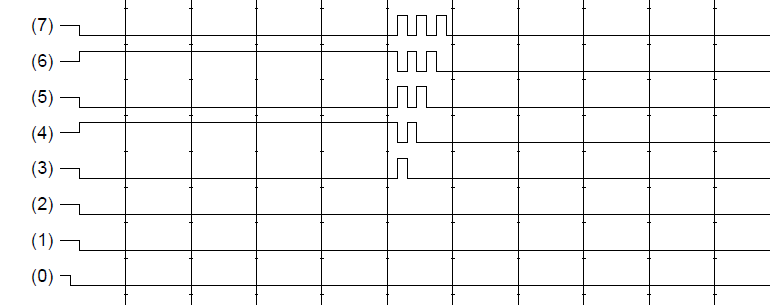
\includegraphics[width=15cm]{./img/Lab_1/Es_2/Glitch_worst_case.png}}
\\\\
In particolare, nell'immagine sopra riportata è possibile osservare come i bit relativi all'uscita di somma, a partire dal
quarto, presentino una continua commutazione fino al raggiungimento del valore logico corretto. La causa di tale comportamento è da ricercare
nelle transizioni a cui gli ingressi sono stati sottoposti nella simulazione. Le due somme, calcolate una di seguito all'altra,
sono le seguenti:
\vspace{0.3cm}
\begin{center}
\begin{tabular}{|c|c|c|}
\hline
& Somma 1 & Somma 2 \\
\hline
Addendo 1 & 10101000 & 00000100\\
\hline
Addendo 2 & 10101000 & 11111100\\
\hline
Risultato & 01010000 & 00000000\\
\hline
Carry in & 01010000 & \\
\hline
\end{tabular}
\end{center}
\vspace{0.3cm}
In particolare è possibile osservare che la somma 2 è soggetta ad una propagazione di carry dal terzo bit in poi, inoltre è importante tenere
in considerazione i carry in ingresso agli stadi lasciati dal risultato della somma 1, in quanto questi saranno una potenziale fonte di glitch propagandosi anch'essi lungo gli stadi. \\\\
In questo caso, la combinazione di carry lasciati dal calcolo precedente e la nuova operazione richiesta (somma 2) fanno si che il sommatore risulti in una condizione per cui, ad ogni colpo di clock, le uscite degli stadi successivi al secondo continueranno a commutare in modo alternato fino a che il carry introdotto dalla seconda operazione non raggiungerà il suddetto stadio, portando così
il bit di somma ad un risultato finale. 
\\\\
Si può notare che i primi 3 bit non sono affetti da tale fenomeno, questi infatti non sono soggetti alla propagazione di carry derivanti dalle due somme. È possibile ricostruire una situazione simile per questi primi bit, ponendo in ingresso un susseguirsi di due
somme leggermente differenti dalle precedenti:
\vspace{0.3cm}
\begin{center}
\begin{tabular}{|c|c|c|}
\hline
& Somma 1 & Somma 2 \\
\hline
Addendo 1 & 10101010 & 00000001\\
\hline
Addendo 2 & 10101010 & 11111111\\
\hline
Risultato & 01010100 & 00000000\\
\hline
Carry in & 01010100 & \\
\hline
\end{tabular}
\end{center}
\vspace{0.3cm}
In tal modo il fenomeno di propagazione dei carry e delle commutazioni delle uscite di somma è esteso anche per i bit meno significativi. Di seguito è riportato un risultato della simulazione ottenuto ponendo tali valori in ingresso al sommatore.
\\\\\\
\centerline{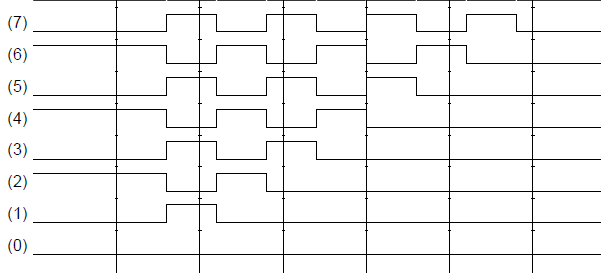
\includegraphics[width=12cm]{./img/Lab_1/Es_2/Worst_case_nostro.png}}
\newpage
\section{Sintesi e analisi di potenza di un RCA}
È possibile effettuare una stima di potenza avanzata attraverso la piattaforma Synopsys. 
Partendo infatti dalla descrizione VHDL del RCA fornito, il software è in grado di compiere una sintesi ottimizzata e mappare il circuito su una libreria di celle caratterizzate dal punto di vista di area, consumi e ritardi.
\\\\
Per poter stimare la potenza dinamica è necessario conoscere la frequenza di lavoro del circuito, ottenuta valutando il percorso combinatorio con ritardo maggiore: è possibile ottenere tale parametro attraverso un timing report.
Il ritardo massimo riportato è pari a 0.78ns, di conseguenza è stato scelto un periodo di clock pari a 1ns.\\
Successivamente è possibile procedere con l'analisi relativa alla potenza.
Il comando power report consente di ottenere una generica stima della potenza dissipata dal circuito, distinguendo tre contributi:
\begin{itemize}
\item \textbf{leakage}: consumo statico dovuto alle correnti di leakage dei dispositivi utilizzati
\item \textbf{internal}: contributo di potenza dinamica dovuto al consumo interno delle celle utilizzate per la sintesi del circuito, comprende al suo interno il contributo di corrente di corto circuito
\item \textbf{switching}: contributo alla potenza dinamica dovuto alle commutazioni dei nodi e alle relative cariche/scariche delle capacità
\end{itemize}
Nella seguente tabella è riportata la suddivisione dei tre contributi.
\\
\begin{center}
	\begin{tabular}{|c|c|c|c|}
	\hline
	Switching Power & Internal Power & Leakage Power & Total Power \\ 
	\hline
	9.7406 uW & 16.7429 uW & 953.4833 nW & 27.4370 uW \\
	\hline
	\end{tabular}
\end{center}
\vspace{0.3cm}
L'apporto maggiore al consumo totale è dato dalla potenza dinamica, in particolare dal consumo della potenza interna.\\
È interessante notare la suddivisione del consumo in potenza per i vari moduli interni (FA) dell'RCA. È possibile ottenere ciò tramite un power report di tipo gerarchico. La distribuzione dei consumi è riportata nella seguente tabella.
\\
\begin{center}
	\begin{tabular}{|c|c|c|c|c|}
	\hline
	Blocco &  Switching Power & Internal Power & Leakage Power & Total Power \\ 
	\hline
	FA(8) & 0.848 uW & 2.154 uW & 119.291 nW & 3.121 uW  \\
	\hline
	FA(7) & 1.293 uW & 2.150 uW & 118.962 nW & 3.562 uW  \\
	\hline
	FA(6) & 1.332 uW & 2.191 uW & 119.340 nW & 3.642 uW  \\
	\hline
	FA(5) & 1.328 uW & 2.171 uW & 119.110 nW & 3.618 uW  \\
	\hline
	FA(4) & 1.278 uW & 2.101 uW & 119.294 nW & 3.498 uW  \\
	\hline
	FA(3) & 1.263 uW & 2.090 uW & 118.879 nW & 3.471 uW  \\
	\hline
	FA(2) & 1.229 uW & 2.002 uW & 119.508 nW & 3.351 uW  \\
	\hline
	FA(1) & 1.171 uW & 1.884 uW & 119.999 nW & 3.175 uW  \\
	\hline
	RCA & 9.741 uW & 16.743 uW & 953.483 nW & 27.437 uW  \\
	\hline
	\end{tabular}
\end{center}
\vspace{0.3cm}
Si nota come la suddivisione risulti simile per tutti i FA fatta eccezione per FA(8). In particolare quest'ultimo si differenzia dagli altri per il consumo relativo alla potenza di switch. Si ipotizza che quest'ultima risulti inferiore rispetto agli altri full adder a causa del minor carico di uscita.
\\\\
È inoltre possibile approfondire l'analisi di potenza considerando i contributi delle celle interne ai singoli moduli. In particolare, vengono messi in luce i contributi delle celle che compongono i singoli FA, sempre suddivisi nei tre contributi precedentemente descritti.
Per comprendere l'origine del consumo inferiore del FA8, quest'ultimo è stato analizzato attraverso la direttiva cell ed è stato confrontato con FA1.
Lo schema del circuito interno e i risultati ottenuti sono riportati di seguito.
\\\\
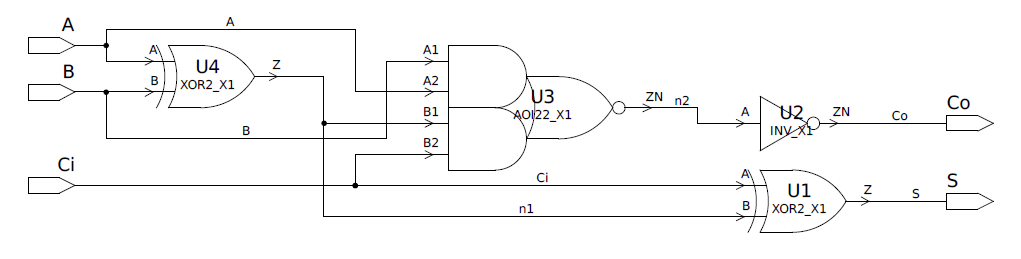
\includegraphics[width=15cm]{./img/Lab_1/Es_3/Full_adder.png}
\\\\
\begin{center}
	\begin{tabular}{|c|c|c|c|c|}
	\multicolumn{5}{c}{FA(1) }\\
	\hline
	Cella &  Switching Power & Internal Power & Leakage Power & Total Dynamic Power \\ 
	\hline
	U4 & 0.5488 uW & 0.5899 uW & 36.1637 nW & 1.138 uW  \\
	\hline
	U3 & 0.1749 uW & 0.3374 uW & 32.5747 nW & 0.512 uW  \\
	\hline
	U2 & 0.3964 uW & 0.1377 uW & 14.2499 nW & 0.534 uW  \\
	\hline
	U1 & 0.0512 uW & 0.8205 uW & 36.0111 nW & 0.872 uW  \\
	\hline
	\end{tabular}
\end{center}
\vspace{0.3cm}
\begin{center}
	\begin{tabular}{|c|c|c|c|c|}
	\multicolumn{5}{c}{FA(8) }\\
	\hline
	Cella &  Switching Power & Internal Power & Leakage Power & Total Dynamic Power \\ 
	\hline
	U4 & 0.5365 uW & 0.5757 uW & 36.1637 nW & 1.112 uW  \\
	\hline
	U3 & 0.2155 uW & 0.4278 uW & 32.7466 nW & 0.643 uW  \\
	\hline
	U2 & 0.0332 uW & 0.1774 uW & 14.2174 nW & 0.211 uW  \\
	\hline
	U1 & 0.0624 uW & 0.9733 uW & 36.1631 nW & 1.036 uW  \\
	\hline
	\end{tabular}
\end{center}
\vspace{0.3cm}
La differenza nel consumo di potenza di switching è individuata nella cella U2, legata al carry in uscita dal singolo FA.
\\
È possibile ottenere informazioni aggiuntive sul calcolo della switching power relativa ai nodi interni ad un modulo con un'analisi di tipo net verbose. In tale analisi sono riportati i contributi capacitivi necessari al calcolo di tale potenza, espressi nodo per nodo.
\\\\
\begin{center}
	\begin{tabular}{|c|c|c|c|c|}
	\multicolumn{5}{c}{FA(1) }\\
	\hline
	Nodo &  Total Net Load & Static Probability & Toggle Rate & Switching Power \\ 
	\hline
	n1 & 4.694 fF & 0.493 & 0.1932 & 0.5488 uW  \\
	\hline
	n2 & 2.010 fF & 0.488 & 0.1439 & 0.1749 uW  \\
	\hline
	S & 0.310 fF & 0.507 & 0.2735 & 0.0512 uW  \\
	\hline
	Cout & 4.554 fF & 0.512 &  0.1439 & 0.3964 uW  \\
	\hline
	\end{tabular}
\end{center}
\vspace{0.3cm}
\begin{center}
	\begin{tabular}{|c|c|c|c|c|}
	\multicolumn{5}{c}{FA(8) }\\
	\hline
	Nodo &  Total Net Load & Static Probability & Toggle Rate & Switching Power \\ 
	\hline
	n1 & 4.694 fF & 0.499 & 0.1889 & 0.5365 uW  \\
	\hline
	n2 & 2.010 fF & 0.484 & 0.1772 & 0.2155 uW  \\
	\hline
	S & 0.310 fF & 0.497 & 0.3328 & 0.0624 uW  \\
	\hline
	Cout & 0.310 fF & 0.516 &  0.1772 & 0.0332 uW  \\
	\hline
	\end{tabular}
\end{center}
\vspace{0.3cm}
Si nota come il nodo legato al carry in uscita presenti una capacità inferiore per FA8. Ciò conferma l'ipotesi legata al carico inferiore.
\\
Analizzando i vari FA con analisi di tipo net verbose si nota inoltre che i contributi di capacità relativi ai nodi della somma (S) siano trascurabili rispetto agli altri contributi.
Di conseguenza si evince che il contributo di potenza relativo a tale nodo è di un ordine di grandezza inferiore rispetto agli altri.
\\\\
Da un report di tipo net verbose è inoltre possibile confrontare i valori di static probability e toggle rate dei nodi di uscita di un FA.
\\
Si nota come i valori di probabilità dei
nodi di uscita, S e Cout, siano distribuiti attorno al valore 0.5, dunque confrontabili con il caso teorico caratterizzato ingressi equiprobabili precedentemente analizzato.
\\\\
Il toggle rate rappresenta la frequenza media di commutazione associata al singolo nodo, che identifica, con il suo reciproco, il periodo medio
con cui tale nodo presenta una commutazione: attraverso tale valore è possibile stimare la switching activity dei nodi di somma e dei carry in uscita.
\\
In tal caso, poichè il periodo di clock è pari a 1ns, il valore di toggle rate riportato coincide con la switching activity del segnale.
\\\\
È possibile notare come i valori simulati si distanzino da quelli teorici, in quanto all'interno del metodo probabilistico non viene tenuta in considerazione la correlazione spaziale e temporale tra diversi segnali. Tale fatto mette in luce, di conseguenza, le limitazioni che l'utilizzo di un modello probabilistico comporta.
\\\\
È stato richiesto inoltre un power report di tipo net verbose relativo all'intero RCA. Si osserva come i contributi capacitivi relativi
ai nodi delle uscite di somma siano significativamente inferiori rispetto ai contributi dei nodi relativi ai carry tra uno stadio e quello successivo.
Anche in questo caso la motivazione è dovuta al carico capacitivo inferiore delle uscite di somma, che non risultano collegate ad ulteriori
blocchi. Tuttavia, osservando i contributi di potenza riportati dall'analisi di tipo verbose, è possibile osservare una differenza tra questi e 
quelli presenti nel power report precedentemente richiesto. 
\\
\begin{center}
	\begin{tabular}{|c|c|c|c|c|}
	\hline
	& Internal Power & Switching Power & Leakage Power & Total Power \\ 
	\hline
	Power report & 16.7429 uW & 9.7406 uW & 953.4833 nW & 27.4370 uW \\
	\hline
	Net Verbose & 8.848 uW & 3.766 uW & 403.098 nW & 12.614 uW \\
	\hline
	\end{tabular}
\end{center}
\vspace{0.3cm}
I contributi riportati dall'analisi di tipo net verbose risultano proporzionalmente inferiori. La possibile causa di ciò è da attribuirsi al tipo
di analisi effettuata da Synopsys: in particolare la keyword \textbf{-net} utilizzata ha richiesto uno studio della potenza relativo ai nodi interni
dell'architettura dell'RCA, presenti tra i vari FA connessi. In tale analisi i contributi delle celle stesse e dei nodi interni ai FA sono stati
tralasciati. Al contrario un'analisi di tipo power report fornisce un risultato completo comprendendo all'interno l'analisi di tutti i nodi dei
blocchi che compongono l'architettura.
\newpage
\section{MUX: generazione e propagazione di glitch}
L'obiettivo di questo esercizio è lo studio delle conseguenze 
introdotte dai ritardi delle porte, in particolare all'interno del
multiplexer rappresentato nella seguente figura.
\\\\\
\centerline{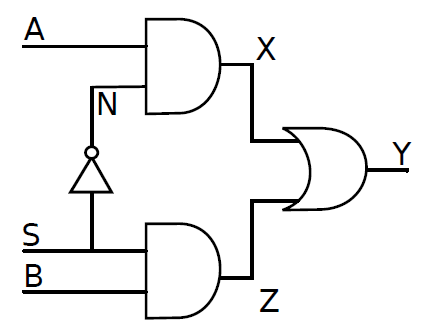
\includegraphics[width=5cm]{./img/Lab_1/Es_4/Mux.png}}
\\\\\
In questo caso particolare tutte le porte sono esenti da ritardi fatta
eccezione per l'inverter, caratterizzato da un ritardo di propagazione
pari a 0.1 ns.
\\\\
All'interno del file \textit{tb\textunderscore mux21\textunderscore
glitch.vhd} è stato possibile identificare la combinazione 
dei segnali di ingresso con i quali il multiplexer è stato
testato.
\begin{center}
\begin{listato}
	\centerline{\lstinputlisting{./code/Lab_1/Es_4/mux_input_delays.vhd}}
\end{listato}
\end{center}
In particolare, è possibile notare dal codice VHDL sopra riportato
che inizialmente gli ingressi assumono tutti un valore logico alto.
Dopo 1ns il segnale S commuta. L'uscita, in un caso ideale, non dovrebbe
presentare commutazioni.
\\
Tuttavia, si ipotizza che, a causa del ritardo di propagazione introdotto dall'
inverter, vi sia un intervallo temporale in cui i nodi interni X e Z 
assumono entrambi un valore logico basso, portando quindi l'uscita Y a 0. Tale comportamento atteso è mostrato nella seguente figura.
\\\\
\centerline{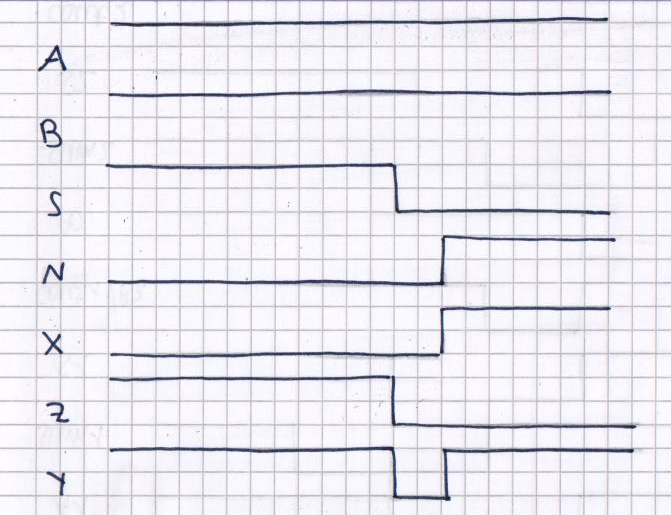
\includegraphics[width=10cm]{./img/Lab_1/Es_4/Mux_plot.png}}
\\\\
Per mezzo di una simulazione ModelSim è stato possibile osservare,
attraverso le waveforms, il comportamento reale dei segnali. Il risultato
di tale simulazione è riportato nella seguente immagine.\\
\\\\
\centerline{\includegraphics[width=7cm]{./img/Lab_1/Es_4/Glitch.png}}
\\\\
È possibile visualizzare direttamente sulla waveform dell'uscita Y
il glitch causato dall'inverter. Tale comportamento è in linea con 
quanto atteso.
\\\\
Al fine di analizzare altre possibili combinazioni degli ingressi
che possano generare un glitch in uscita, è stata realizzata una 
mappa di Karnaugh rappresentante la funzione logica del multiplexer.
\\\\
\centerline{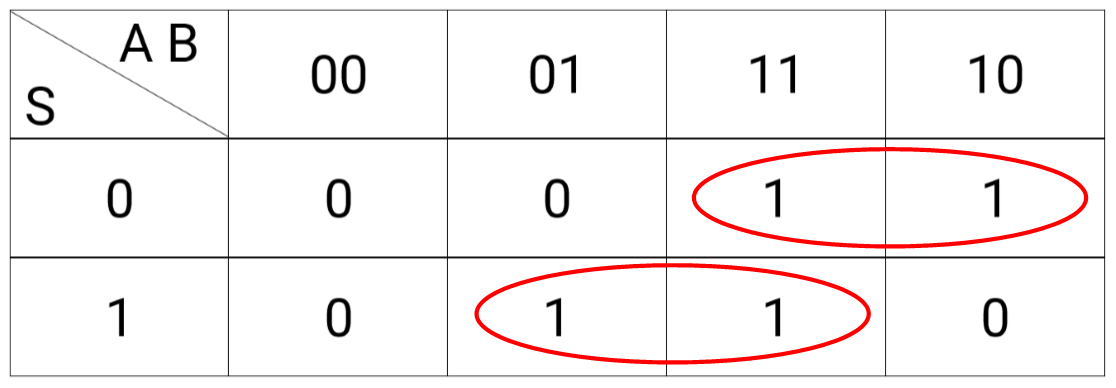
\includegraphics[width=8cm]{./img/Lab_1/Es_4/Mappa_K_coperta.png}}
\\\\
In particolare, è possibile notare che il circuito precedentemente riportato sia l'implementazione della funzione logica coperta da due implicanti, rappresentata nella figura precedente.
\\
Il glitch analizzato è dovuto ad una transizione degli ingressi che consegue in un passaggio
tra un implicante e l'altro. Tale problema potrebbe essere risolto
inserendo, in modo ridondante, un terzo implicante per evitare
la transizione precedentemente trattata. 
\\\\
\centerline{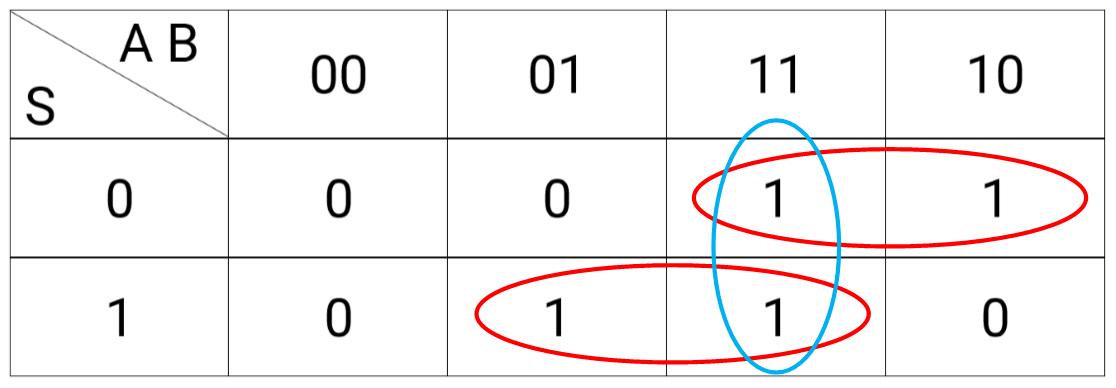
\includegraphics[width=8cm]{./img/Lab_1/Es_4/Mappa_K_supercoperta.png}}
\\\\
Tale ragionamento porta alla conclusione che l'unica combinazione in grado
di causare un glitch in uscita sia quella presa in analisi.
\\\\\
Essendo i glitch associati a commutazioni di nodi, questi portano un 
contributo aggiuntivo al consumo totale di potenza dinamica. In particolare,
l'energia spesa durante queste commutazioni spurie è la somma dei consumi
durante le due transizioni del segnale. Ciascuna delle due contribuisce all'energia secondo la seguente equazione:
\\\\
\centerline{$E = C \cdot V^{2}$}
\\\\
dove C rappresenta la capacità di carico e V la tensione a cui viene caricata
tale capacità.
\\
Metà di tale contributo di energia è usata per caricare o scaricare la
capacità di carico associata all'uscita, mentre la restante parte viene
dissipata.
Di conseguenza il consumo di energia totale associato ad un glitch è 
dato da:
\\\\
\centerline{$E = 2 \cdot C \cdot V^{2}$}
\\\\
\newpage
\section{Calcolo di probabilità e attività: contatore sincrono}
Nella prima parte di questa sezione è stato analizzato il timing del blocco 
rappresentato nella figura seguente.
\\\\
\centerline{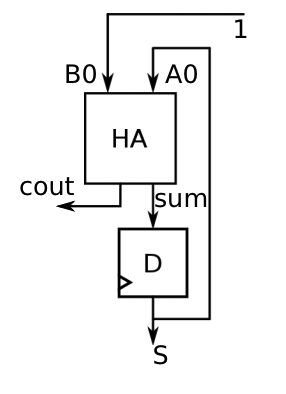
\includegraphics[width=3cm]{./img/Lab_1/Es_5/Sync_FA.png}
			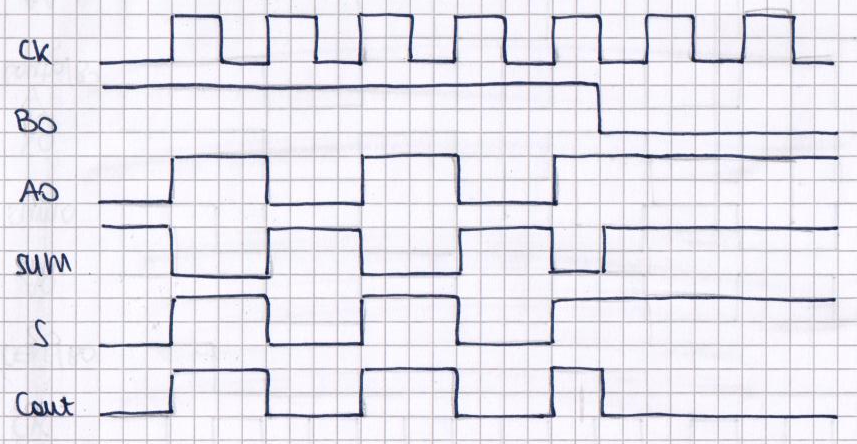
\includegraphics[width=7cm]{./img/Lab_1/Es_5/Half_add_contatore.png}}
\\\\
In particolare, è stato possibile stabilire il suo comportamento atteso. 
Quando il segnale B0 è asserito, l'uscita S presenta una commutazione 
per ogni fronte sensibile del clock. Al contrario, quando B0 non è attivo, 
l'uscita non presenta alcuna commutazione.
\\\\
È possibile utilizzare tali strutture per realizzare un contatore sincrono,
come mostrato in figura. In particolare, i segnali di CEN e OVFL rappresentano
rispettivamente l'enable del contatore e il terminal count di questo.
\\\\
\centerline{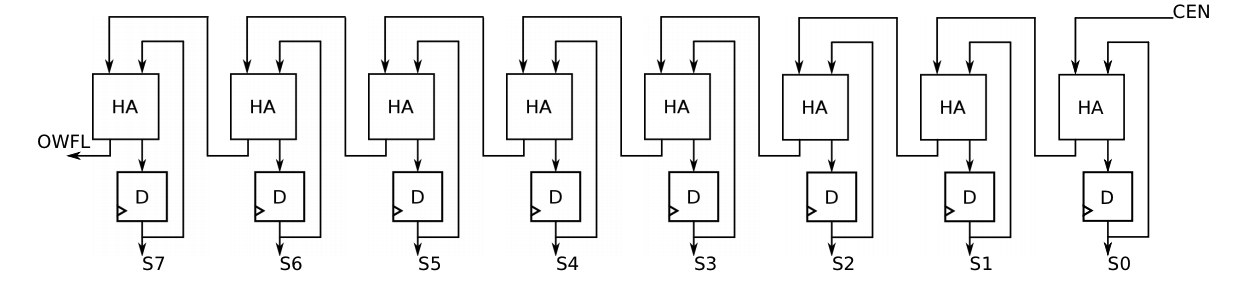
\includegraphics[width=15cm]{./img/Lab_1/Es_5/Counter.png}}
\\\\
Considerando infatti il comportamento delle uscite S0, S1 e S2 quando il segnale di 
enable è attivo si ottiene il seguente timing.
\\\\
\centerline{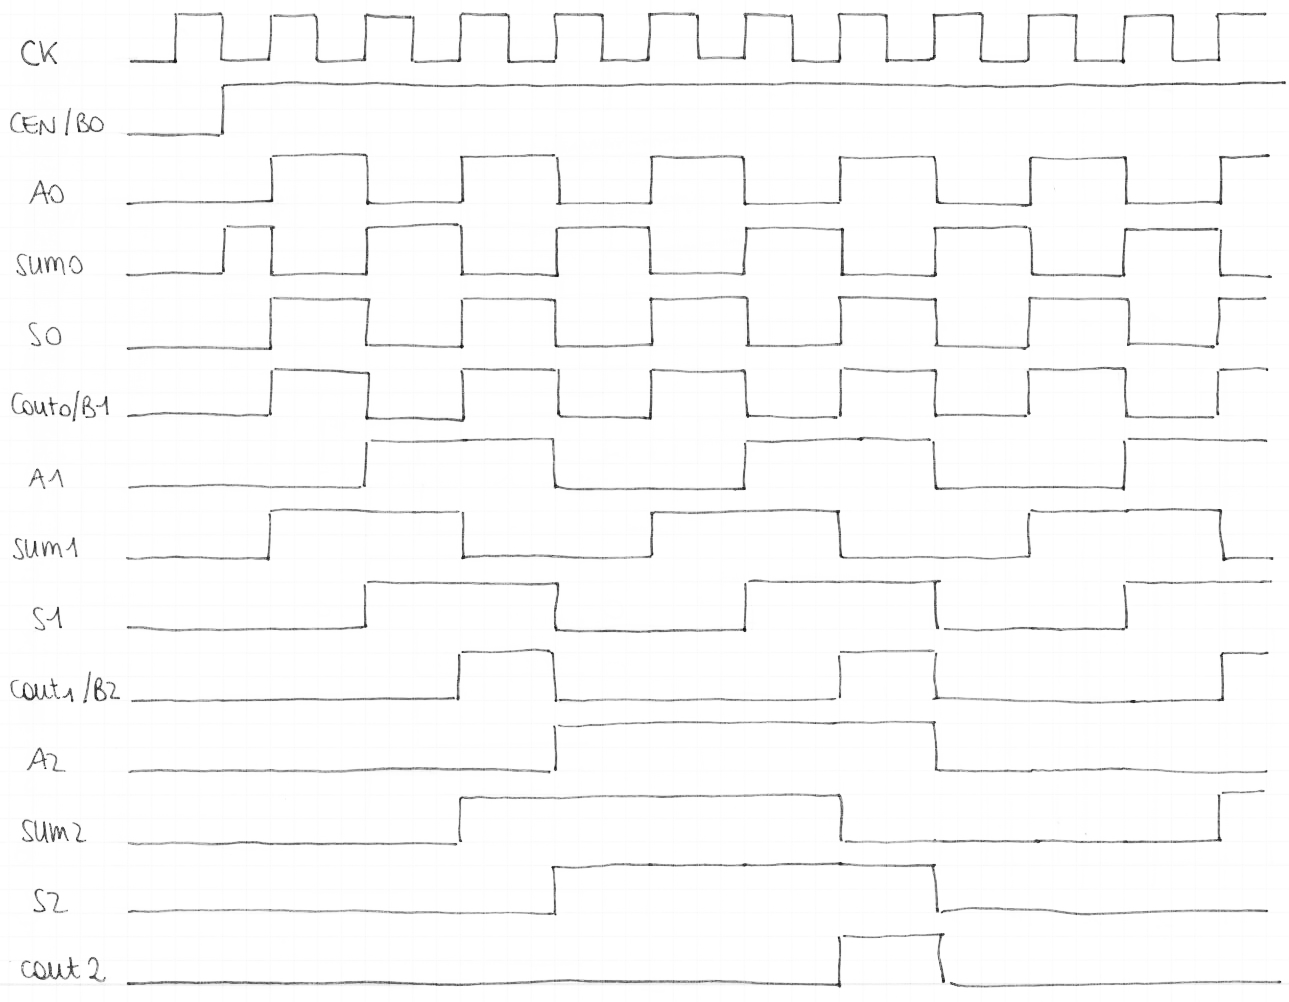
\includegraphics[width=10cm]{./img/Lab_1/Es_5/Contatore.png}}
\\\\
Dalle considerazioni fatte in precedenza è possibile stimare il numero
di commutazioni delle 8 uscite e del terminal count durante 
un intero ciclo di conta.
\\\\Nella tabella seguente sono inoltre stati
aggiunti i dati ottenuti tramite power report, ottenuto attraverso 
una simulazione ModelSim. Il clock utilizzato per la simulazione ha un periodo
di 2ns.
\\
\begin{center}
	\begin{tabular}{|c|c|c|}
	\hline
	Segnale & Transizioni stimate & Transizioni simulate \\ 
	\hline
	S0 & 255 & 257 \\
	\hline
	S1 & 127 & 128\\
	\hline
	S2 & 63 & 64\\
	\hline
	S3 & 31 & 32\\
	\hline
	S4 & 15 & 16 \\
	\hline
	S5 & 7 & 8 \\
	\hline
	S6 & 3 & 4 \\
	\hline
	S7 & 1 & 2 \\
	\hline
	OVFL & 1 & 16 \\
	\hline
	\end{tabular}
\end{center}
\vspace{0.3cm}
Si può notare che, senza considerare il segnale OVFL,
i risultati ottenuti in entrambi i casi siano
confrontabili, tuttavia è presente una leggera differenza, pari
a 1 o 2 colpi di clock, dovuta al fatto che è stato scelto un 
tempo di simulazione leggermente superiore al tempo di conta 
totale.
\\\\
Riguardo al segnale di OVFL, il risultato simulato
è distante da quello atteso, in quanto il segnale presenta un numero di commutazioni
decisamente maggiore. Tale segnale, al contrario delle uscite di somma rappresentanti il conteggio, non 
presenta un elemento sequenziale che lo interfacci con l'esterno. Per tale motivo
sono ben visibili tutte le commutazioni spurie del segnale stesso, dovute ai ritardi
di propagazione definiti all'interno dei vari stati del contatore.
\\\\
Dalla simulazione è stato inoltre possibile osservare l'andamento 
delle waveforms delle uscite, riportato nella figura sottostante.
\\\\
\centerline{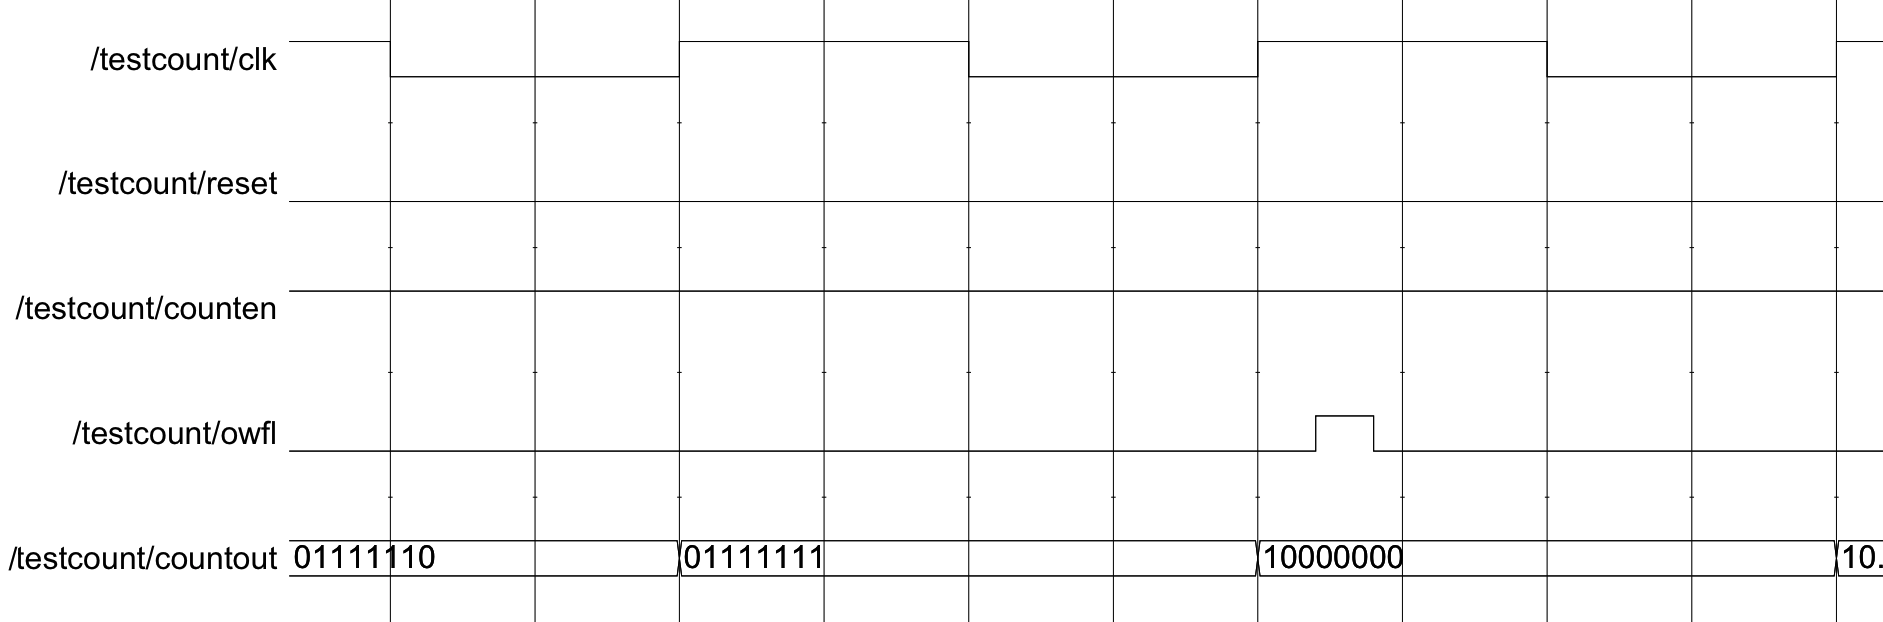
\includegraphics[width=15cm]{./img/Lab_1/Es_5/Glitch.png}}
\\\\
Si nota che, in
un preciso intervallo temporale, il segnale OVFL assume un valore 
logico alto durante il conteggio, comportamento inatteso da parte
di un contatore. 
Tale glitch avviene in seguito alla commutazione
del bit più significativo (S7); infatti, per un certo intervallo di tempo,
in ingresso all'half adder del blocco 7 sono presenti due ingressi con valore
logico alto: uno dovuto al carry in uscita dal blocco precedente che, a causa
dei ritardi, non ha ancora commutato il suo valore, e l'altro relativo all'uscita
attuale S7.
\\\\
Successivamente, sempre attraverso un power report, è stato possibile
analizzare l'attività dei segnali interni al contatore. I risultati sono 
riportati nella seguenti tabelle.
\\
\begin{center}
	\begin{tabular}{|c|c|c|}
	\hline
	Segnale & Commutazioni & Attività \\ 
	\hline
	SUM(0) & 258  & 0.992  \\
	\hline
	SUM(1) & 385  & 1.377  \\
	\hline
	SUM(2) & 320  &  1.231  \\
	\hline
	SUM(3) & 224  & 0.862  \\
	\hline
	SUM(4) & 144  & 0.554  \\
	\hline
	SUM(5) & 88  & 0.338  \\
	\hline
	SUM(6) & 52  & 0.200  \\
	\hline
	SUM(7) & 30  & 0.115  \\
	\hline
	\end{tabular}	
	\begin{tabular}{|c|c|c|}
	\hline
	Segnale & Commutazioni & Attività \\ 
	\hline
	Cout(0) & 257  & 0.988  \\
	\hline
	Cout(1) & 256  & 0.985  \\
	\hline
	Cout(2) & 192  & 0.738  \\
	\hline
	Cout(3) & 128  & 0.492  \\
	\hline
	Cout(4) & 80  & 0.308  \\
	\hline
	Cout(5) & 48  & 0.185  \\
	\hline
	Cout(6) & 28  & 0.108  \\
	\hline
	Cout(7) & 16  & 0.062  \\
	\hline
	\end{tabular}
\end{center}
\vspace{0.3cm}
È possibile notare come l'attività delle somme in uscita dagli
half adder sia differente rispetto alle uscite sincrone dei flip-flop.
Infatti, a causa dei ritardi di propagazione dei carry in uscita dai 
singoli stadi, si generano una serie di glitch, che, propagandosi lungo
la serie di half adder, causano commutazioni multiple dei nodi SUM.
\\\\
Similmente all'analisi effettuata per il blocco 7 è possibile ipotizzare
comportamenti simili legati al carry in uscita anche per gli altri blocchi.
Tale vettore di carry presenta infatti un'attività complessiva maggiore 
rispetto a quella stimata nel caso senza ritardi.
\\\\
Nella simulazione precedentemente effettuata, i ritardi sono stati
modellizzati in modo tale da presentare un valore significativamente
inferiore rispetto al periodo di clock.
\\\\
\centerline{$Periodo = 2ns \\
            Ritardo\textunderscore somma = 0.2ns \\
            Ritardo\textunderscore carry = 0.2ns $}
\\\\
Si nota che, in questo caso, il periodo di clock è 
sufficientemente elevato per garantire un corretto funzionamento 
del contatore: la propagazione del carry out può avvenire correttamente
in tutti gli stadi.
\\\\
Riducendo il periodo di clock a 0.8ns è possibile osservare un
comportamento inatteso, rappresentato in figura, da parte del contatore.
\\\\
\centerline{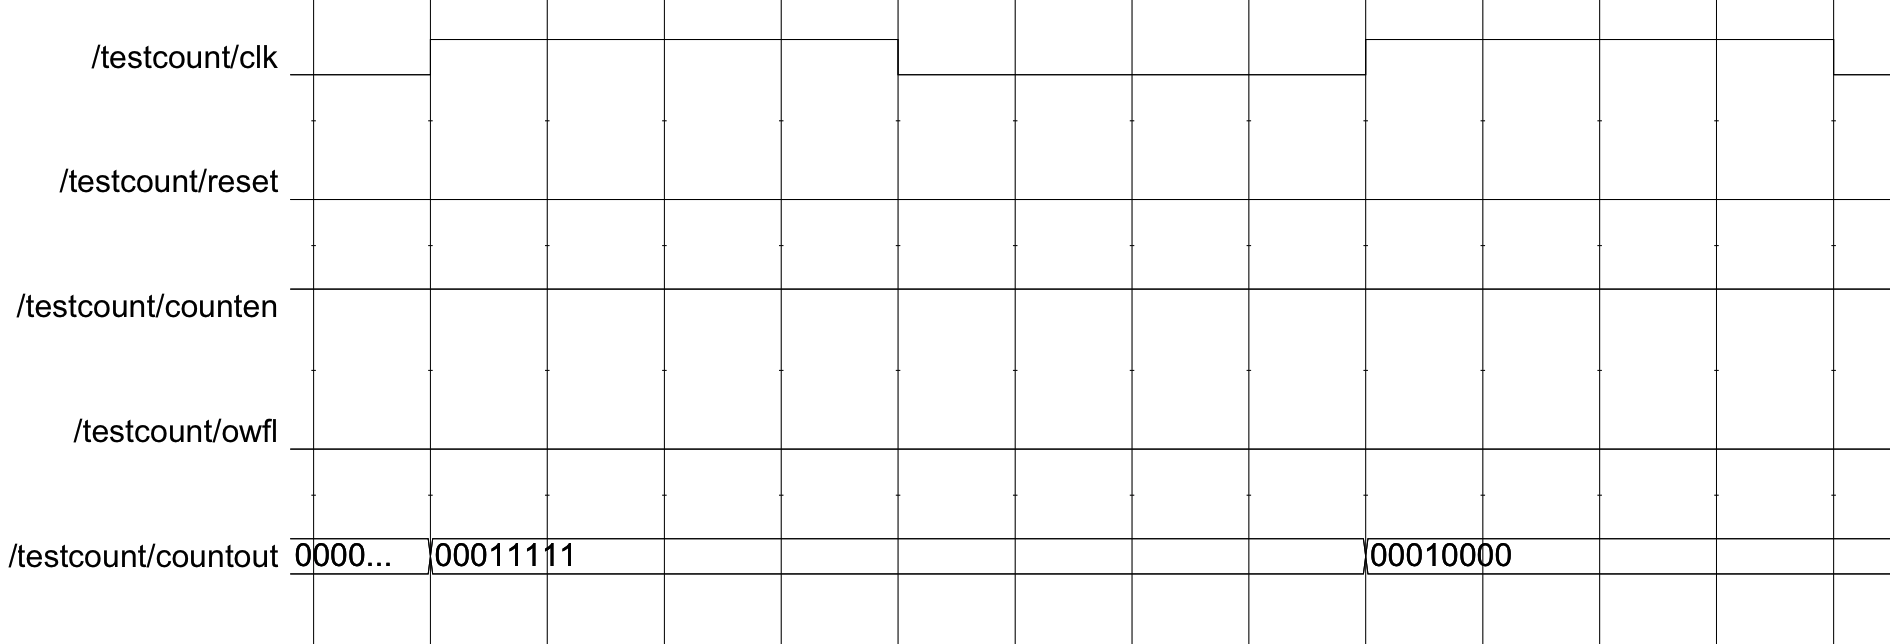
\includegraphics[width=15cm]{./img/Lab_1/Es_5/Clk_corto.png}}
\\\\
L'immagine mette in luce una transizione da un conteggio all'altro:
\\\\
\centerline{$00011111 \rightarrow 00010000$}
\\\\
Tale errore è dovuto alla mancata completa propagazione del carry in tutti
gli stadi, infatti il clock campiona le uscite dei flip-flops prima che tutti
gli stadi abbiano raggiunto un valore stabile. 
\\\\
La presenza di glitch all'interno del contatore in analisi comporta
un incremento dei consumi rispetto al caso ideale. Una possibile soluzione, che potrebbe
essere adottata per garantire un numero inferiore di commutazioni spurie modificando il VHDL, è legata
all'aumento del ritardo coinvolto nel calcolo della somma per i singoli HA. 
Se tale tempo fosse infatti maggiore o uguale del massimo tempo di propagazione 
del carry attraverso tutti gli stadi, le uscite SUM non presenterebbero più un elevato numero di glitch.
\newpage
\chapter{Ottimizzazione FSM e sintesi VHDL}    
\section{FSM State Assignment}
\subsection{Progetto}
L'obiettivo del progetto è la definizione di una macchina  a stati al fine di realizzare un algoritmo di somma tra 6 input, utilizzando il datapath in figura seguente e scegliendo l'ordine con cui collegare i diversi ingressi ai multiplexer.
\\\\
\centerline{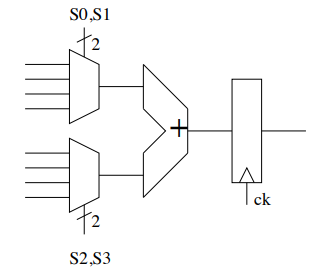
\includegraphics[width=8cm]{./img/Lab_2/Datapath.png}}
\\\\   
In particolare, al fine di minimizzare i consumi della macchina a stati, è necessario ridurre al minimo il numero di commutazioni di:
\begin{itemize}
\item variabili di stato
\item segnali di controllo
\end{itemize} 
Essendo i segnali di controllo coincidenti con i selettori dei multiplexer, è stata innanzitutto stabilita una sequenza per la selezione dei diversi input tale per cui il numero di commutazioni durante l'esecuzione dell'intero algoritmo di somma fosse minimo.
\begin{center}
	\begin{tabular}{|c|c|c|c|c|}
	\hline
	Operazione & S3 & S2 & S1 & S0 \\ 
	\hline
	A+B & 0 & 1 & 0 & 1 \\
	\hline
	S+C & 0 & 0 & 0 & 0  \\
	\hline
	S+D & 0 & 0 & 1 & 0  \\
	\hline
    E+S & 1 & 0 & 1 & 1  \\
	\hline
	F+S & 1 & 1 & 1 & 1 \\
	\hline
	\end{tabular}	
\end{center}
\vspace{0.3cm}     
È possibile notare come sia necessario riportare il valore della somma, denominato S, in ingresso ad entrambi i multiplexer.
\\
Nella transizione da uno stato all'altro il numero di commutazioni coincide con la variazione degli addendi; ne consegue che il massimo numero di commutazioni durante una transizione risulta pari 2.\\
Considerando un ciclo di esecuzione dell'algoritmo, è possibile stimare il numero totale di commutazioni sui segnali di selezione e la loro switching activity.\\
\begin{center}
	\begin{tabular}{|c|c|c|c|c|}
	\hline
	 & S3 & S2 & S1 & S0 \\ 
	\hline
	Commutazioni in un ciclo & 2 & 2 & 2 & 2 \\
	\hline
	Attività & 0.4 & 0.4 & 0.4 & 0.4  \\
	\hline
	\end{tabular}	
\end{center}
\vspace{0.3cm}  
Il numero di commutazioni totale risulta quindi pari a 8.\\
È stata scelta dunque la seguente configurazione degli ingressi 
\\\\
\centerline{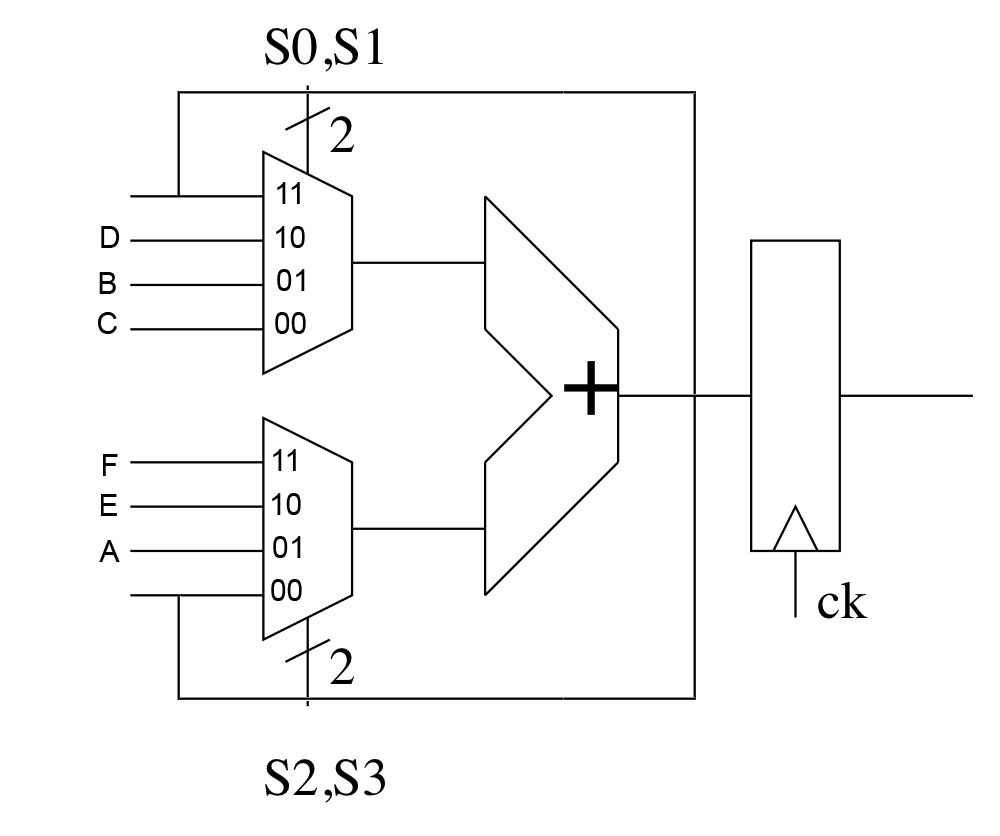
\includegraphics[width=8cm]{./img/Lab_2/Datapath_input.png}}
\\\\  
Il passo successivo è la scelta della codifica dei singoli stati. In tale contesto è importante tenere in considerazione che una generica FSM presenta una rete per la generazione degli output e una rete per il calcolo dello stato futuro. 
\\\\
Una codifica ottimale punta alla minimizzazione delle commutazioni in entrambe le reti. Per tale scopo si è deciso di far coincidere le due reti, in modo che la logica utilizzata per generare le uscite possa essere sfruttata anche per la definizione dello stato futuro. In particolare, la codifica dello stato futuro si ottiene a partire dalle uscite di controllo dello stato attuale.
\\
\begin{center}
	\begin{tabular}{|c||c||c|c|c|c|}
	\hline
	Operazione & Codifica dello stato & S3 & S2 & S1 & S0 \\ 
	\hline
	A+B & 1 1 1 & 0 & 1 & 0 & 1 \\
	\hline
	S+C & 1 0 1 & 0 & 0 & 0 & 0 \\
	\hline
	S+D & 0 0 0 & 0 & 0 & 1 & 0 \\
	\hline
	E+S & 0 1 0 & 1 & 0 & 1 & 1 \\
	\hline
	F+S & 0 1 1 & 1 & 1 & 1 & 1 \\
	\hline
	\end{tabular}	
\end{center}
\vspace{0.3cm}  
È possibile notare come tutte le transizioni presentino una distanza di Hamming pari a 1, fatta eccezione della transizione da S+C a S+D, nella quale tale distanza è pari a 2.
\\
In tale contesto, la sola logica combinatoria necessaria è relativa alla valutazione delle uscite a partire dalla codifica dello stato attuale.
\\\\
Si è notato che tali funzioni logiche presentano un'implementazione semplice con un numero limitato di porte. Di seguito sono riportate le mappe di Karnaugh per le funzioni logiche sopra descritte.
\\\\
\centerline{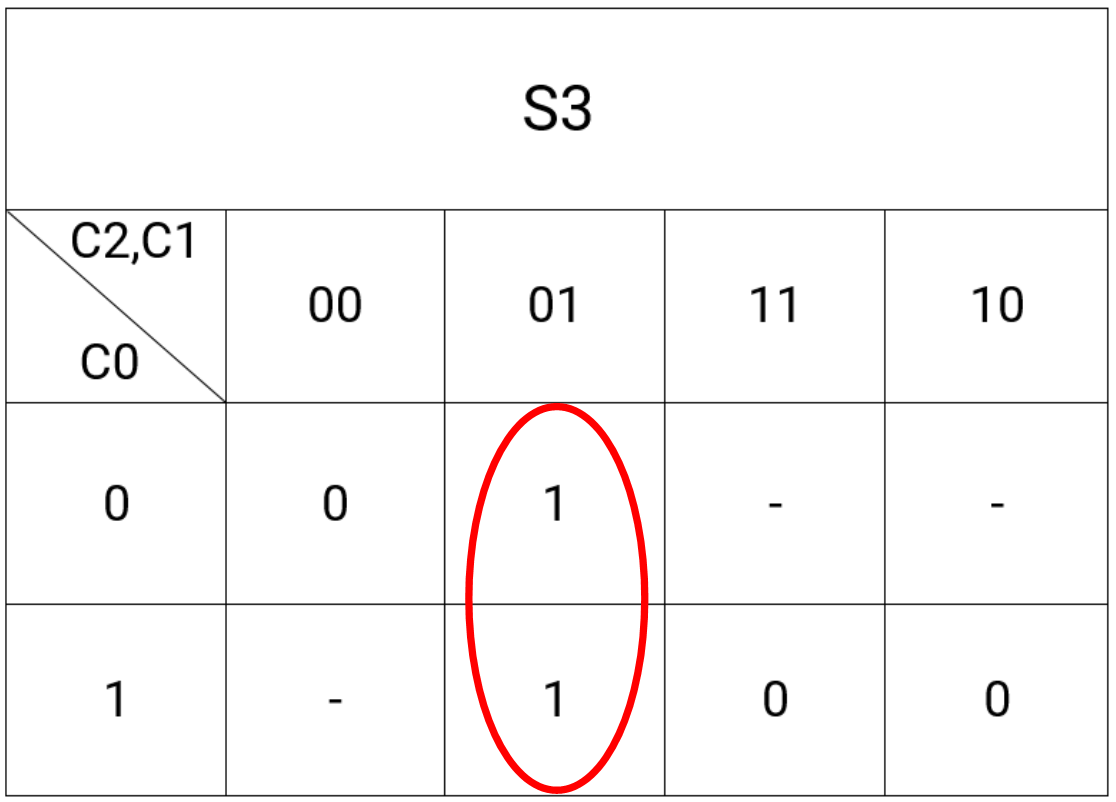
\includegraphics[width=7cm]{./img/Lab_2/K_S3.png}
			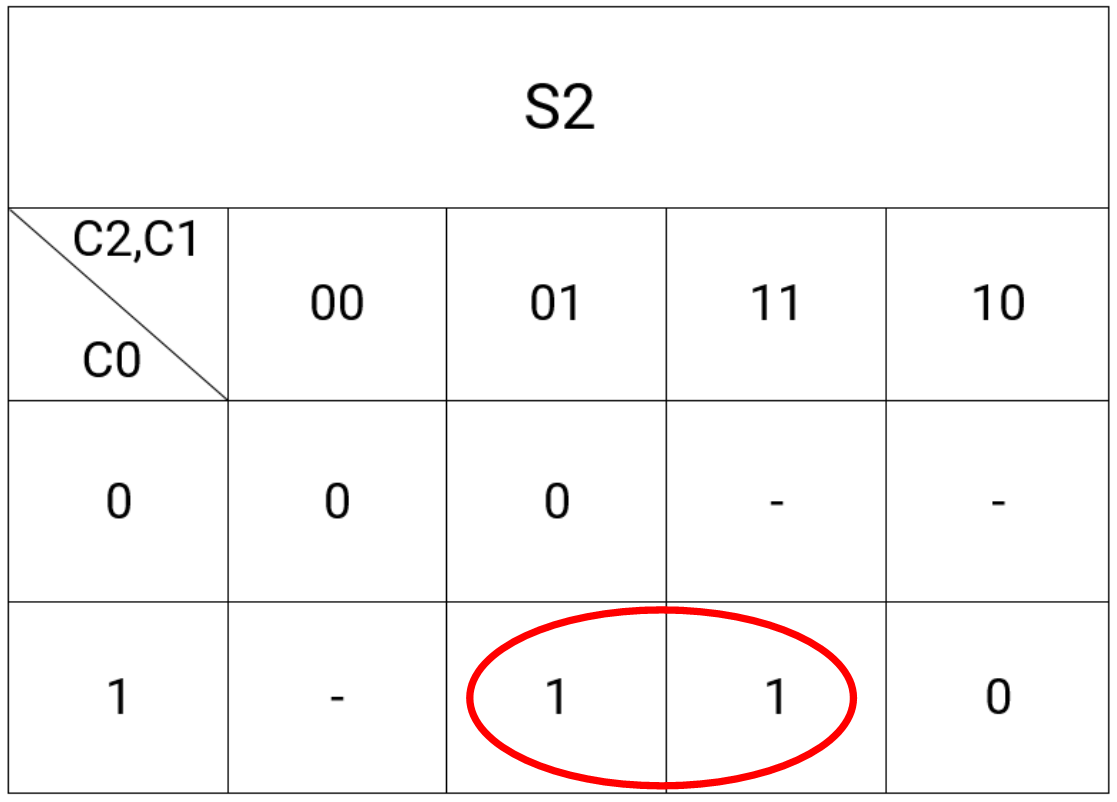
\includegraphics[width=7cm]{./img/Lab_2/K_S2.png}}
\\\\
\centerline{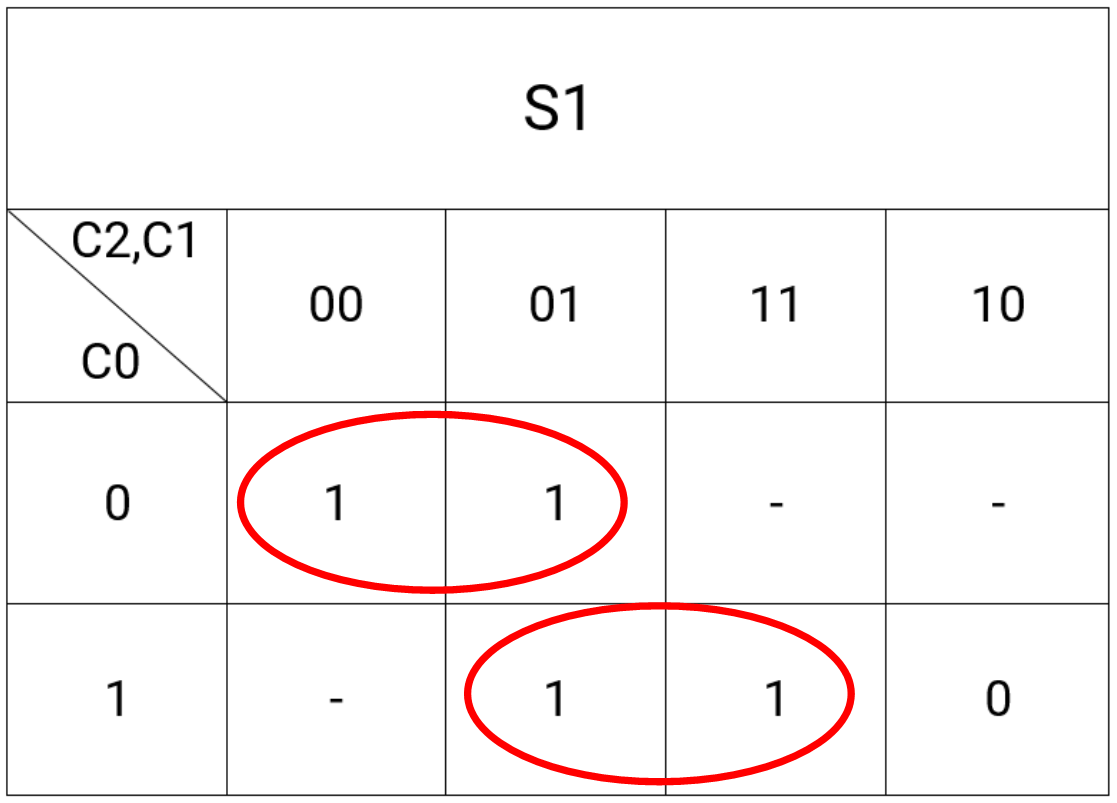
\includegraphics[width=7cm]{./img/Lab_2/K_S1.png}
			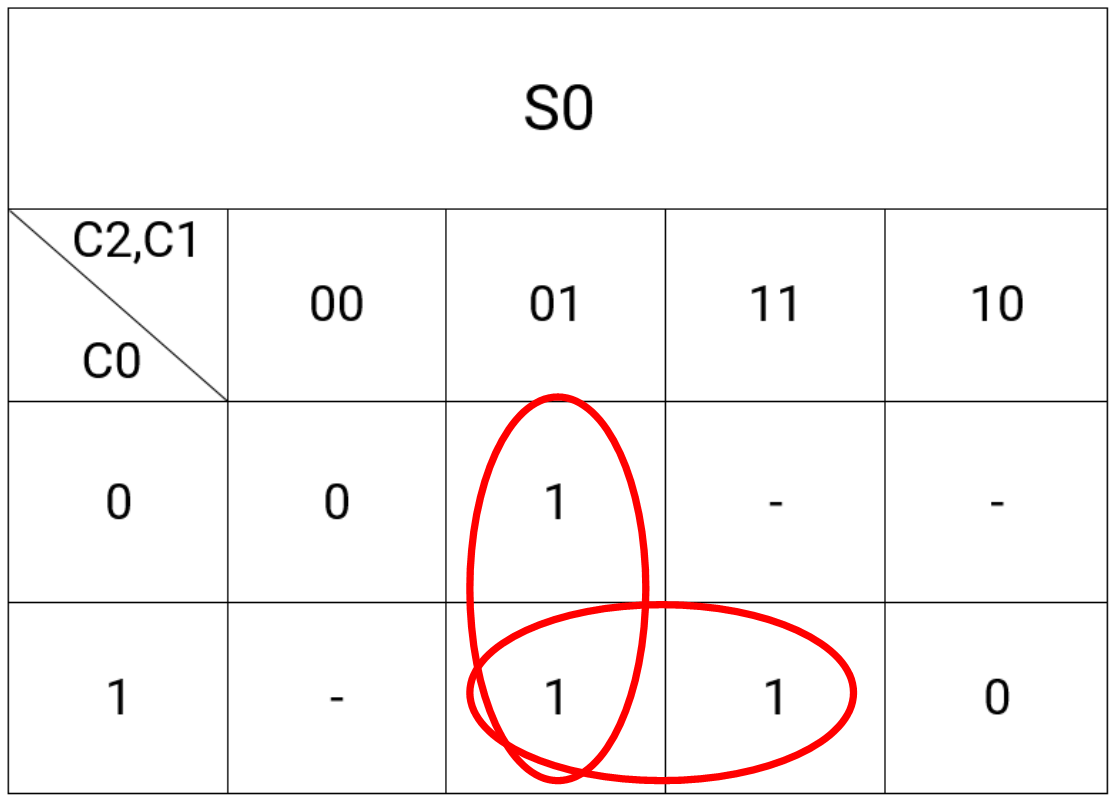
\includegraphics[width=7cm]{./img/Lab_2/K_S0.png}}
\\\\
È possibile notare che le funzioni logiche presentano implicanti in comune, semplificando maggiormente la logica necessaria.
\\
\subsection{Descrizione VHDL e simulazione Modelsim}
La macchina a stati precedentemente definita è stata descritta in VHDL, specificando in particolare la codifica degli stati progettata.
\\
Il codice implementato è riportato nell'Appendice A alla sezione \textit{Laboratorio 2 - FSM}.
\\\\
Al fine della simulazione, datapath e FSM sono stati inclusi in un'unica entity per ottenere il Processing Element complessivo. È stato dunque realizzato un testbench (riportato nell' Appendice A alla sezione \textit{Laboratorio 2 - FSM}) per verificare il corretto susseguirsi degli stati e le relative transizioni dei segnali.
In particolare, è stata effettuata una simulazione di 2000 colpi di clock, che ha fornito i seguenti risultati attraverso un power report.
\\
\begin{center}
	\begin{tabular}{|c|c|c|}
	\hline
	Segnale & Tc & Activity \\ 
	\hline
	Clock & 4000 & 2 \\
	\hline
	S3 & 799 & 0.3995 \\
	\hline
	S2 & 802 & 0.4010 \\
	\hline
	S1 & 799 & 0.3995 \\
	\hline
	S0 & 802 & 0.4010 \\
	\hline
	\end{tabular}	
\end{center}
\vspace{0.3cm}  
Le attività ottenute sono comparabili con quelle stimate in fase di progetto.  
\\
\section{Sintesi del VHDL} 
In tale sezione è stata effettuata la sintesi della top level entity che comprende sia FSM sia datapath.
\\
Inizialamente i file sono stati analizzati nel corretto ordine ed è stata elaborata la struttura del Processing Element.
\\
Successivamente è stato generato un clock di periodo pari a 10 ns.
\\\\
\centerline{\textbf{create\_clock -name "CLK" -period 10 {CLK}} }
\\\\
È stata verificata la presenza del clock generato attraverso il comando \textbf{report\_clock}.
\\\\
Successivamente è stata effettuata la sintesi attraverso la direttiva \textbf{compile -exact map}.
\\
Dunque è stato possibile visualizzare, in modo gerarchico, la mappatura del circuito con la libreria scelta. Nell'immagine seguente, in particolare, è riportato lo schematico della macchina a stati.
\\\\
\centerline{\includegraphics[width=15cm]{./img/Lab_2/FSM_Schematic.png}}
\\\\ 
È possibile notare, come atteso, che il numero di porte logiche utilizzato risulta limitato.
\\
Sono stati effettuati una serie di report inizialmente sulla top level entity per poi analizzare in modo più approfondito la macchina a stati.
\\
In primo luogo è stata ottenuta una stima dell'area delle celle utilizzate nella sintesi, attraverso il comando \textbf{report\_area}.
\\\\
\centerline{Total cell area = 295.53 um$^2$}
\\\\
Successivamente, al fine di valutare lo slack, sono stati analizzati i 10 percorsi combinatori con ritardi maggiori.
\\\\
\centerline{\textbf{report\_timing -nworst 10}}
\\\\
Per semplicità sono riportati i dati relativi al critical path.
\\
\begin{center}
	\begin{tabular}{|c|c|}
	\hline
	Clock period & 10 ns\\
	\hline
	Data required time & 9.97 ns \\
	\hline
	Data arrival time & 1.94 ns \\
	\hline
	Slack & 8.02 ns \\
	\hline
	\end{tabular}	
\end{center}
\vspace{0.3cm}  
Come è possibile notare, lo slack risulta particolarmente elevato se confrontato con il periodo di clock.
Nel report sono inoltre presenti i ritardi relativi agli elementi compresi tra lo start-point e l'end-point del percorso critico.
\\\\
È possibile ottenere informazioni riguardo alla potenza dissipata attraverso il comando \textbf{report\_power}. In particolare, si evidenziano i tre contributi relativi alla top level entity.
\\
\begin{center}
	\begin{tabular}{|c|c|}
	\hline
	Internal Power & 29.4711 uW \\
	\hline
	Switching Power & 13.2924 uW \\
	\hline
	Leakage Power & 5.4747 uW \\
	\hline
	Total Power & 48.2382 uW \\
	\hline
	\end{tabular}	
\end{center}
\vspace{0.3cm}  
Sono stati ottenuti dati aggiuntivi relativi al consumo di potenza dei singoli moduli dell'architettura, tramite l'aggiunta della direttiva \textbf{-hier}.
\begin{center}
	\begin{tabular}{|c|c|c|}
	\hline
	FSM & 4.504 uW & 9.3\% \\
	\hline
	Datapath & 43.734 uW & 90.7\% \\
	\hline
	\end{tabular}	
\end{center}
\vspace{0.3cm}  
Il consumo della macchina a stati rappresenta una percentuale ridotta rispetto al valore totale.
\\
Al fine di approfondire lo studio relativo ai nodi interni del circuito, è stata realizzata un'analisi di tipo \textbf{-net}. In particolare sono riportati i risultati relativi ai nodi dei segnali di selezione dei multiplexer, che costituicono il contributo preponderante.
\\
\begin{center}
	\begin{tabular}{|c|c|c|c|c|}
	\hline
	Segnale & Net Load [fF] & Static Probability & Toggle Rate & Switching Power [uW] \\
	\hline
	 sel11\_wire & 13.792  &  0.120  &  0.0246  & 0.2055 \\
	\hline
	 sel01\_wire & 10.222  &  0.253  &  0.0272  & 0.1682 \\
	\hline
	sel10\_wire & 8.489  &  0.720  &  0.0301  & 0.1547\\
	\hline
	sel00\_wire & 7.058  &  0.720  &  0.0301  & 0.1286 \\
	\hline
	\end{tabular}	
\end{center}
\vspace{0.3cm}
Il periodo medio di variazione dei selettori, ottenibile dal toggle rate, è confrontabile con le variazioni medie che avvengono su tali segnali in un ciclo di esecuzione. È importante tenere in considerazione la possibile presenza di commutazioni non previste a causa dell'attivazione del segnale di reset durante la simulazione, il quale è caratterizzato da una probabilità non nulla di commutazione. Per ottenere una stima realistica sarebbe necessario infatti caratterizzare le attività dei nodi con risultati legati al comportamento reale del circuito.
\\\\
È possibile imporre dei vincoli sui vari parametri coinvolti nel processo di sintesi. In particolare, è stato generato un segnale di clock alla massima frequenza consentita dal circuito. La stima di tale frequenza è stata effettuata a partire dall'analisi del critical path precedentemente riportata.
\\
\begin{center}
	\begin{tabular}{|c|c|}
	\hline
	Clock period & 1.94 ns\\
	\hline
	Data required time & 1.91 ns \\
	\hline
	Data arrival time & 1.91 ns \\
	\hline
	Slack & 0 ns \\
	\hline
	\end{tabular}	
\end{center}
\vspace{0.3cm} 
Come atteso, lo slack relativo al percorso critico risulta essere nullo, di conseguenza il circuito opera alla massima frequenza supportata.
Dal momento che la potenza dissipata è funzione della frequenza di lavoro, è stato riscontrato un aumento dei consumi.
\\
\begin{center}
	\begin{tabular}{|c|c|}
	\hline
	Internal Power & 151.3501 uW \\
	\hline
	Switching Power & 69.4127 uW \\
	\hline
	Leakage Power & 5.5735 uW \\
	\hline
	Total Power & 226.3363 uW \\
	\hline
	\end{tabular}	
\end{center}
\vspace{0.3cm} 
A seguito di un incremento della frequenza di un fattore di circa 5, la potenza è aumentata proporzionalmente. In particolare si riscontra come risultato la proporzionalità tra frequenza e consumo di potenza dinamico.
\\\\
È inoltre possibile imporre un vincolo sul contributo totale di potenza dinamica, attraverso la direttiva:
\\\\
\centerline{\textbf{set\_max\_dynamic\_power}}
\\\\
Tale valore è stato fissato a 40 uW, leggermente inferiore rispetto alla potenza dinamica ottenuta nelle prime simulazioni.
\\
In particolare, è stato considerato il clock di partenza di periodo pari a 10 ns.
Di seguito sono riportati i risultati ottenuti.
\\
\begin{center}
	\begin{tabular}{|c|c|c|}
	\hline
	& No constraints & Power constraints\\
	\hline
	Internal Power & 29.4711 uW & 33.8116 uW \\
	\hline
	Switching Power & 13.2924 uW & 13.3092 uW \\
	\hline
	Total Dynamic Power & 42.76 uW & 47.12 uW \\
	\hline
	\end{tabular}	
\end{center}
\vspace{0.3cm}  
I risultati ottenuti dalla sintesi non risultano in linea con quanto atteso, infatti è registrato un aumento del consumo di potenza dinamica.
\\
Si ipotizza che il consumo di potenza dinamica ottenuto nella prima sintesi fosse già prossimo al minimo globale.
\\\\
Successivamente, è stata effettuata un'analisi più dettagliata della FSM accedendovi tramite la direttiva\textbf{ current\_instance FSM}.\\
Attraverso il comando \textbf{report\_fsm} è stato possibile verificare la corretta implementazione della codifica progettata.
\\\\
È possibile risalire alla suddivisione del consumo della potenza dinamica all'interno delle celle che costituiscono la FSM attraverso un'analisi di potenza di tipo \textbf{-cell}. In particolare, nella seguente tabella vengono riportati i tre contributi maggiori relativi al consumo di potenza dinamica.
\\
\begin{center}
	\begin{tabular}{|c|c|}
	\hline
	  ps\_reg[1] & 1.143 uW  \\
	\hline
	 ps\_reg[2] & 0.979 uW\\
	\hline
	ps\_reg[0] & 0.924 uW\\
	\hline
	\end{tabular}	
\end{center}
\vspace{0.3cm}
Si nota che tali contributi sono relativi alle variabili di stato, che presentano numerose commutazioni durante l'esecuzione dell'algoritmo.
\\\\
Uno studio più approfondito sulla switching power relativa ai nodi interni è ottenuta tramite un'analisi di tipo \textbf{-net}. In particolare, nella seguente tabella, sono riportati i dati relativi ai segnali di uscita della FSM, ovvero i segnali di selezione dei multiplexer.
\\
\begin{center}
	\begin{tabular}{|c|c|c|c|c|}
	\hline
	Segnale & Net Load [fF] & Static Probability & Toggle Rate & Switching Power [uW] \\
	\hline
	 S11 & 13.792  &  0.120  &  0.0246  & 0.2055 \\
	\hline
	 S01 & 10.222  &  0.253  &  0.0272  & 0.1682 \\
	\hline
	S10 & 8.489  &  0.720  &  0.0301  & 0.1547\\
	\hline
	S00 & 7.058  &  0.720  &  0.0301  & 0.1286 \\
	\hline
	\end{tabular}	
\end{center}
\vspace{0.3cm}
È possibile notare che tali valori coincidono con quelli ottenuti precedentemente durante l'analisi -net della top level entity. Il contributo maggiore del consumo è dovuto alle capacità di carico dei nodi in analisi, che assumono  valori significativi rispetto agli altri nodi. Questo è il principale motivo per cui tali segnali contribuiscono maggiormente, considerando che il toggle rate risulta confrontabile.
\\\\
Per ragioni di praticità, tali sintesi sono state effettuate raggruppando i comandi e le direttive in uno script in modo da rendere il processo automatico. Di seguito è riportato uno degli script utilizzati.
\begin{center}
\begin{listato}
	\centerline{\lstinputlisting{./code/Lab_2/commands.txt}}
\end{listato}
\end{center}

\chapter{Clock gating e soluzioni architetturali}
\section{Un primo approccio al clock gating}
Il clock gating è una tecnica di riduzione dei consumi a livello architetturale, il cui scopo è impedire la commutazione del segnale di clock in determinate parti del circuito non utilizzate.
\\
È fornita una descrizione VHDL del seguente circuito.
\\
\centerline{\includegraphics[width=8cm]{./img/Lab_3/circuito_clk_bug.png}}
\\
Dal file VHDL è possibile notare il valore assegnato ai segnali D1, D2 e D3:
\begin{center}
\begin{listato}
	\centerline{\lstinputlisting{./code/Lab_3/d1_d2_d3.vhd}}
\end{listato}
\end{center}
Essendo il segnale di clock enable sempre attivo, è atteso che l'uscita D3 assuma un valore pari a D1 dopo due cicli di clock. Tale comportamento non è verificato da una prima simulazione ModelSim effettuata.
\\
Come possibile notare dalla seguente figura, al primo fronte attivo di clock successivo al reset, il valore di D1 è già riportato in uscita al flip-flop controllato dal segnale di strobe.
\\\\
\centerline{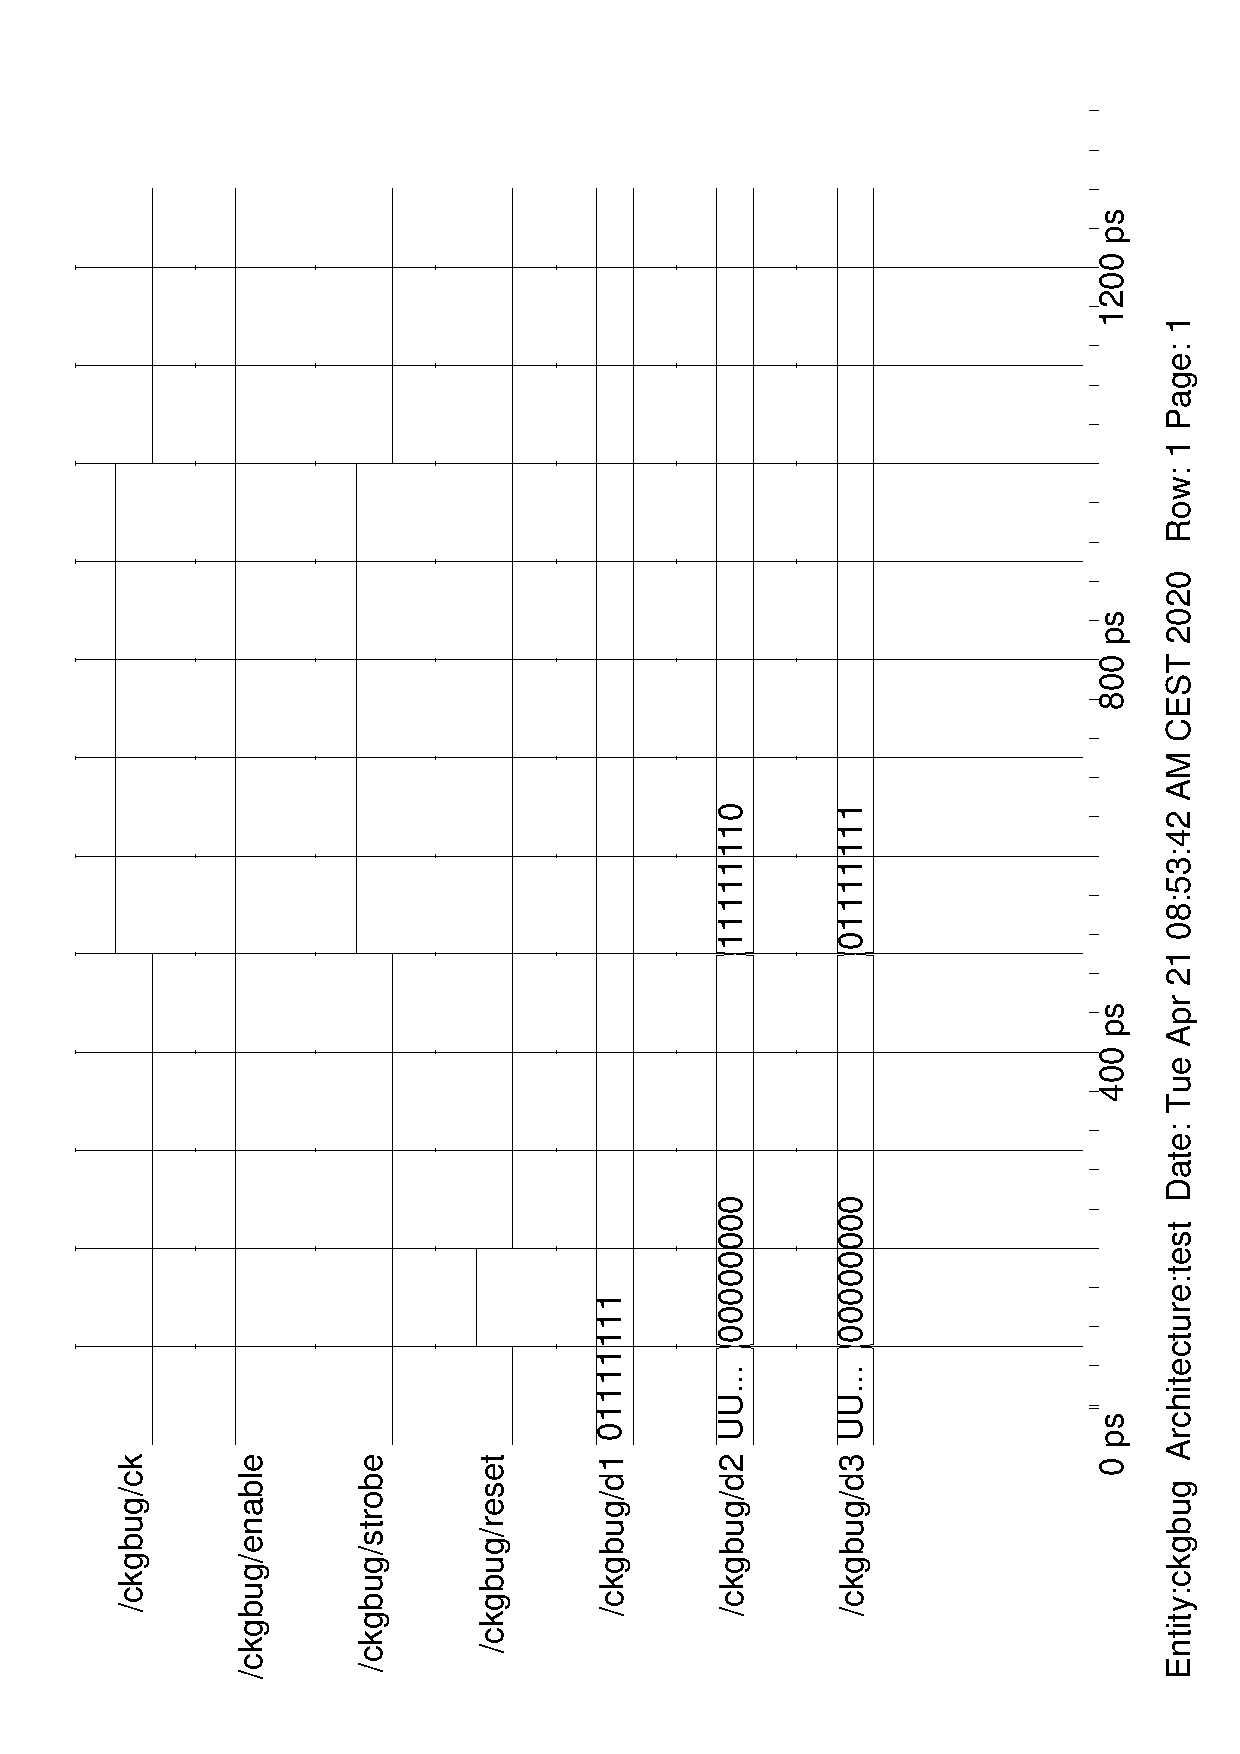
\includegraphics[width=10cm]{./img/Lab_3/clk_bug.png}}
\\\\
Ciò accade poiché il simulatore, in assenza di informazioni sui ritardi, deve comunque simulare il circuito mantenendo una causalità nella propagazione dei segnali all'interno degli elementi descritti.
\\
Come conseguenza, l'informazione relativa al clock, a causa della presenza di una porta AND, è riportata all'ingresso del secondo flip-flop uno step di simulazione dopo rispetto al primo. Tale comportamento è deleterio in quanto altera il timing previsto del circuito.
\\\\
Per assicurare il corretto funzionamento del circuito, è sufficiente indicare la presenza di un ritardo CK $\rightarrow$ Q per entrambi i flip-flop. A tale scopo è stato modificato il file \textbf{fd.vhd}.
\begin{center}
\begin{listato}
	\centerline{\lstinputlisting{./code/Lab_3/ff_delay.vhd}}
\end{listato}
\end{center}
Il ritardo aggiunto sulla propagazione dell'uscita permette di raggiungere il risultato atteso dalla simulazione.
\\\\
\centerline{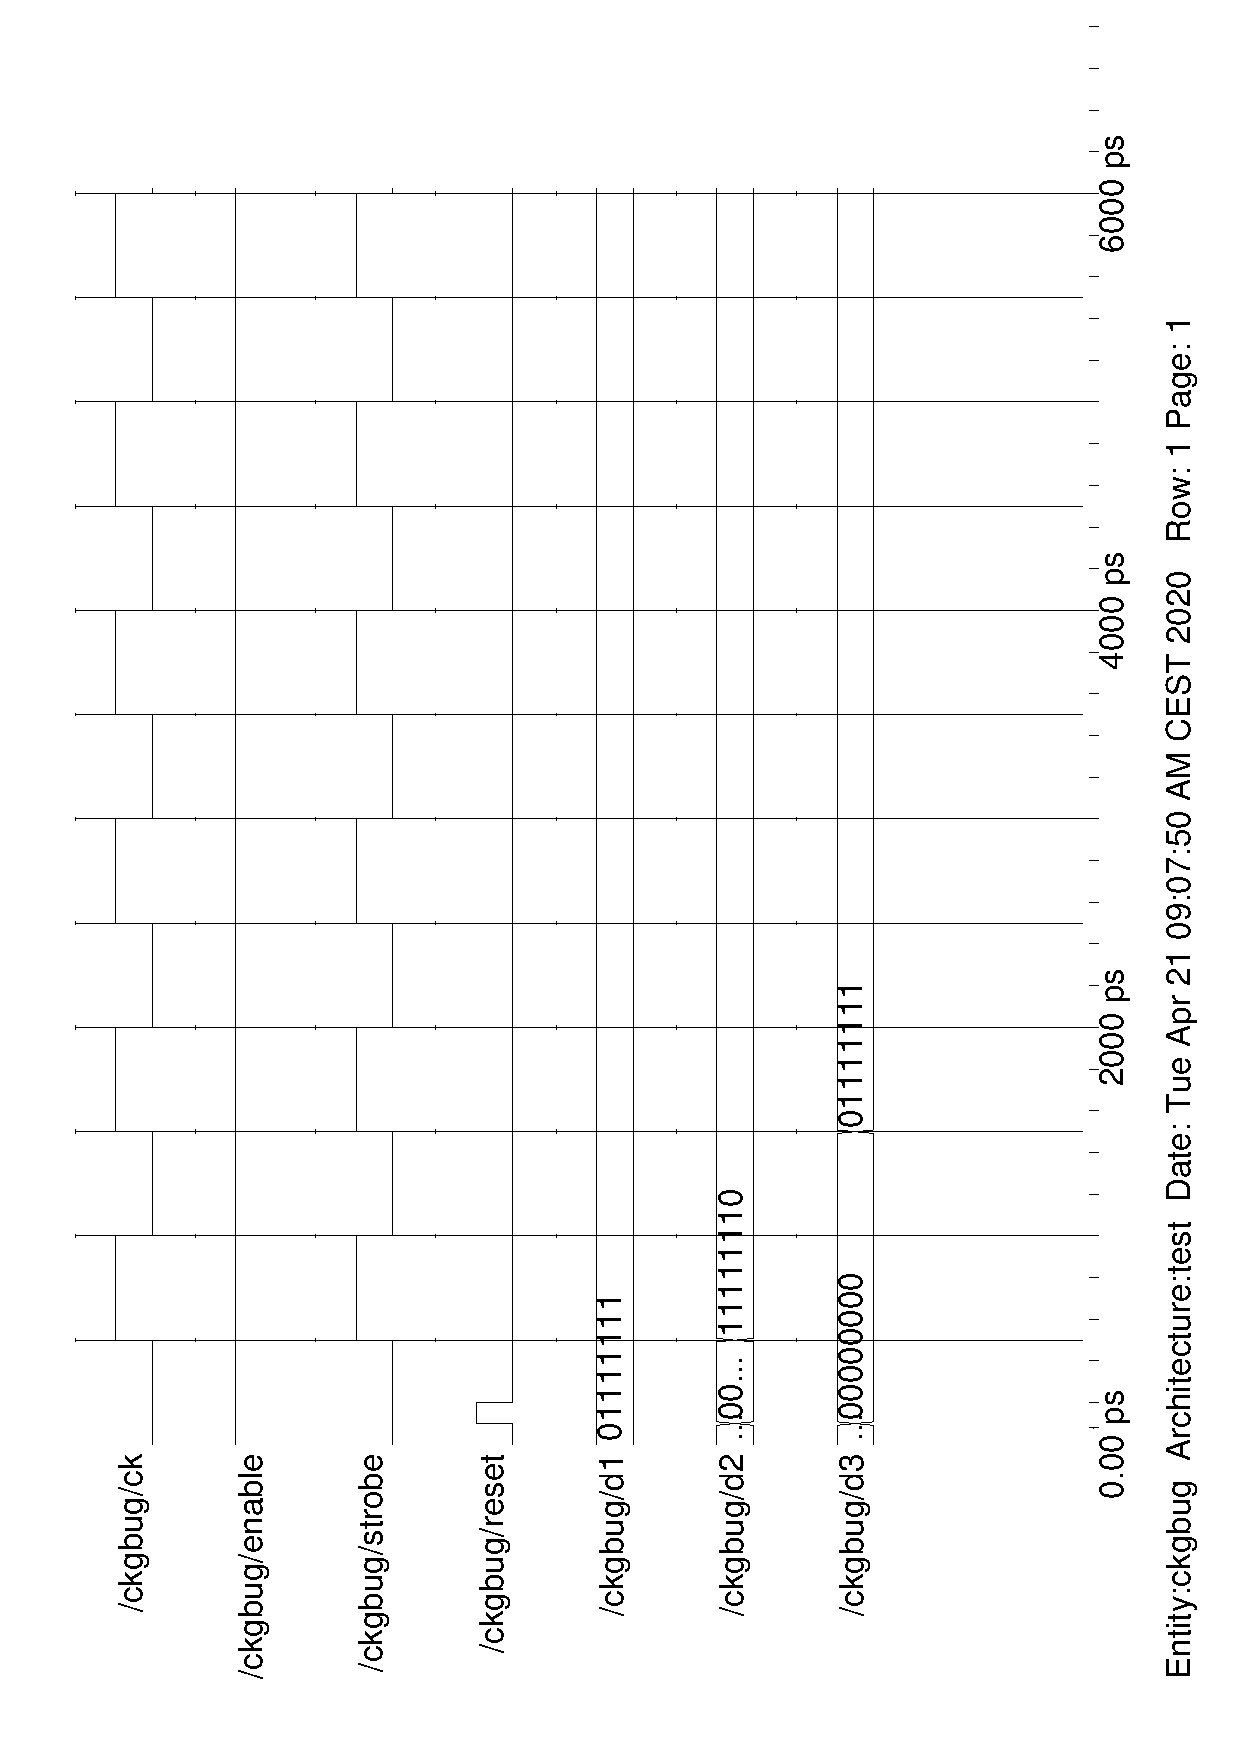
\includegraphics[width=10cm]{./img/Lab_3/clk_bug_resolved.png}}
\\\\
Se la porta AND è caratterizzata da un ritardo maggiore rispetto al ritardo CK $\rightarrow$ Q precedentemente inserito, il valore campionato in uscita non è quello corretto. In particolare, l'errore riscontrato è analogo a prima, come mostrato nella seguente figura.
\\\\
\centerline{\includegraphics[width=10cm]{./img/Lab_3/clk_bug_delay.png}}
\newpage
\section{Clock gating per un circuito complesso}
\subsection{Simulazione del circuito}
All'interno del file \textbf{inccomp.vhd} è presente una descrizione del circuito mostrato nella figura seguente.
\\\\
\centerline{\includegraphics[width=10cm]{./img/Lab_3/inccomp_no_gating.png}}
\\\\
Dal codice si evince che il circuito è in grado di incrementare e confrontare due valori, rappresentati su 8 bit, contenuti nei registri A e B, e portare il maggiore di essi in uscita. In particolare, l'operazione di incremento è gestita attraverso INCA e INCB, due segnali attivi alti.
\\
È stato realizzato un testbench con lo scopo di simulare e verificare il comportamento del circuito.
\\\\
\centerline{\includegraphics[width=12cm]{./img/Lab_3/inccomp_no_gating_behavior.png}}
\\\\
Come possibile notare dalle forme d'onda sopra riportate, il comportamento è in linea con quanto atteso.
\\ 
Infatti, il segnale INCA viene campionato per tre colpi di clock prima che INCB risulti attivo, ciò porta il valore contenuto in REG\_A uguale a 3. In seguito, asserendo INCB, anche il valore contenuto in REG\_B inizia ad aumentare. Nei cicli di clock in cui entrambi INCA e INCB sono asseriti, la differenza tra i due dati rimane costante. Nel momento in cui INCA viene negato, il valore in uscita dal circuito rimane costante fino a che il dato contenuto in REG\_B risulti maggiore: questo accade esattamente dopo tre cicli di clock.
\\\\
Nel caso in cui i segnali di incremento non siano asseriti, non è necessario far commutare il clock all'interno dei registri, in quanto nessun valore deve essere aggiornato; a tal proposito, è possibile sfruttare la tecnica del clock gating. Una possibile implementazione è mostrata nella seguente figura.
\\\\
\centerline{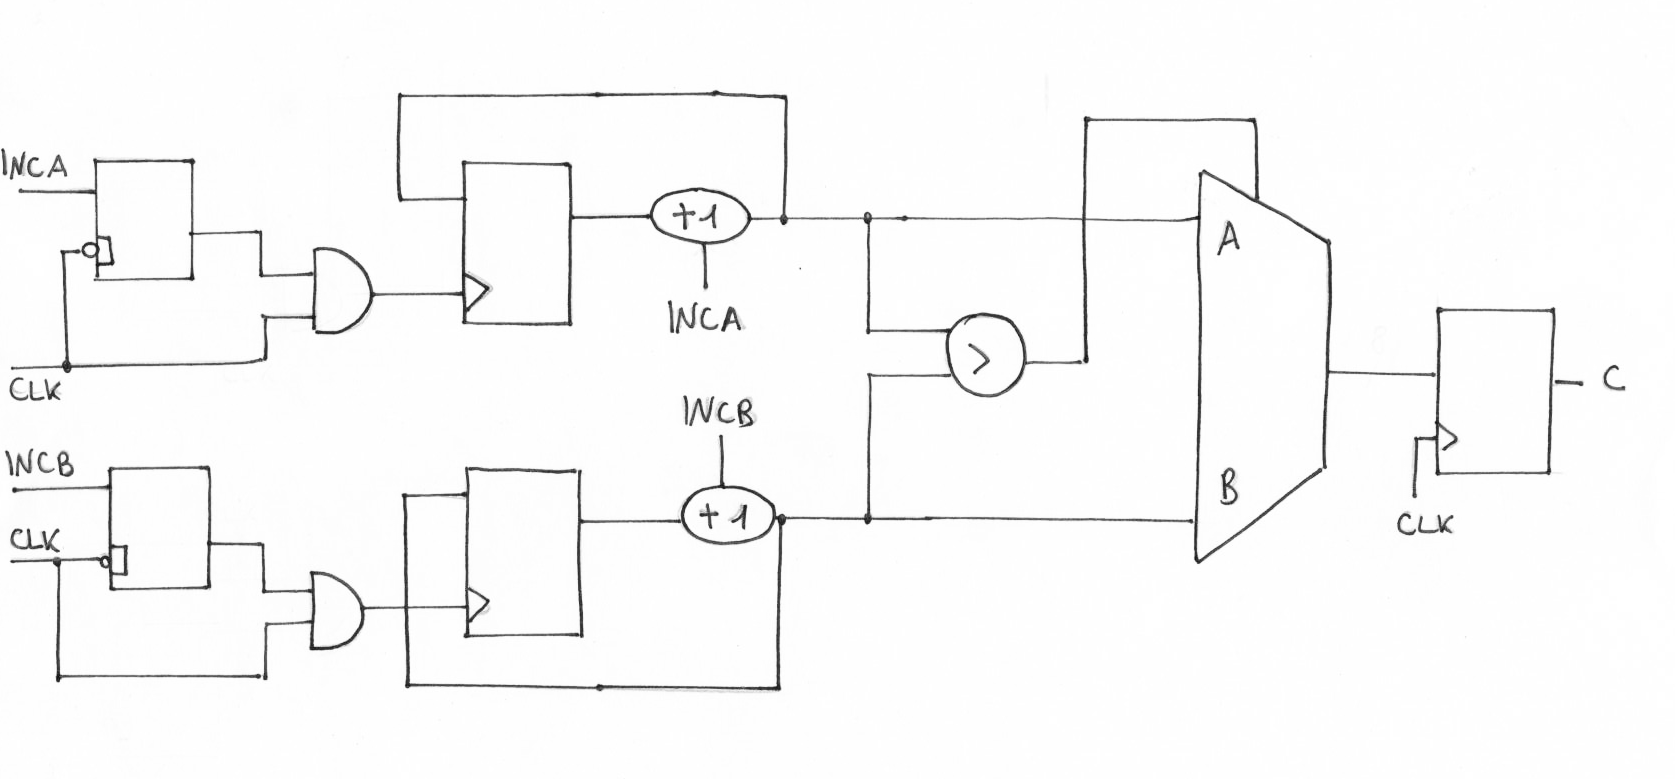
\includegraphics[width=10cm]{./img/Lab_3/Clk_gating_img.png}}
\\\\
È possibile notare la presenza di due latch atti a filtrare eventuali glitch presenti sugli ingressi INCA e INCB.
\subsection{Sintesi del circuito}
Inizialmente è stata effettuata una sintesi in assenza di direttive per l'implementazione del clock gating.
Successivamente alla generazione di un clock di periodo pari a 5 ns, è stato effettuato un power report includendo anche il contributo dei nodi relativi agli ingressi attraverso la direttiva \textbf{-include\_input\_net}.
\\
\begin{center}
	\begin{tabular}{|c|c|c|c|}
	\hline
	\multicolumn{4}{|c|}{Power report - no clock gating, statistica di default} \\
	\hline
	Internal power [uW] & Net switching power [uW] & Leakage power [uW] & Total power [uW] \\
	\hline
	 38.7514 & 13.6944  &  3.7969  &  56.2428 \\
	\hline
	\end{tabular}	
\end{center}
\vspace{0.3cm}
Un'analisi di potenza di tipo \textbf{-net} permette di ottenere informazioni più dettagliate sulla statistica dei segnali e sulle capacità coinvolte. 
\\
In particolare, si nota che le capacità relative ai nodi di ingresso assumono un valore significativo, di conseguenza è importante tenere in considerazione tali nodi in una stima di potenza.
\\
Sono riportate le informazioni statistiche relative ai segnali di clock, reset, INCA e INCB.
\\
\begin{center}
	\begin{tabular}{|c|c|c|}
	\hline
Segnale & Static probability & Toggle rate \\
	\hline
	 clock & 0.5  &  0.4 \\
	\hline
	 reset & 0.5  &  0.02 \\
	\hline
	 INCA & 0.5  &  0.02 \\
	\hline
	 INCB & 0.5  &  0.02 \\
	\hline
	\end{tabular}	
\end{center}
\vspace{0.3cm}
Tali valori non sono realistici rispetto ai segnali presi in considerazione.
\\
È possibile effettuare stime più accurate comunicando al sintetizzatore i dati statistici relativi ai segnali. In particolare, è stata inizialmente modificata la statistica del segnale di reset, impostando la static probability pari a 0.
\\
\begin{center}
	\begin{tabular}{|c|c|c|c|}
	\hline
	\multicolumn{4}{|c|}{Power report - no clock gating, reset modificato}\\
	\hline
	Internal power [uW] & Net switching power [uW] & Leakage power [uW] & Total power [uW] \\
	\hline
	 27.6360 & 14.8140  & 4.18  &  46.6302 \\
	\hline
	\end{tabular}	
\end{center}
\vspace{0.3cm}
In seguito, impostando le statistiche relative ai segnali INCA e INCB con static probability pari a 0.12 e toggle rate pari a 0.025, come specificato nella consegna, si ottengono i seguenti risultati.
\\
\begin{center}
	\begin{tabular}{|c|c|c|c|}
	\hline
	\multicolumn{4}{|c|}{Power report - no clock gating, reset e ingressi modificati}\\
	\hline
	Internal power [uW] & Net switching power [uW] & Leakage power [uW] & Total power [uW] \\
	\hline
	21.5273 & 10.8718  & 4.0921  &  36.4911 \\
	\hline
	\end{tabular}	
\end{center}
\vspace{0.3cm}
Si nota una sensibile riduzione dei consumi dovuti al minor numero di commutazioni medie dei segnali in ingresso.\\
Per ottenere il numero totale di celle utilizzato dal sintetizzatore, è stata realizzata un'analisi di tipo \textbf{-cell}.
\\
\begin{center}
	\begin{tabular}{|c|c|}
	\hline
	Numero celle & Area [um$^2$] \\
	\hline
	 74 & 229.29 \\
	\hline
	\end{tabular}	
\end{center}
\vspace{0.3cm}
Attraverso una particolare descrizione VHDL, è possibile notificare al sintetizzatore la possibilità di implementare, attraverso opportune celle, la tecnica del clock gating, che può essere richiesta nella fase di sintesi attraverso la direttiva \textbf{-gate\_clock}.
Utilizzando sempre un clock di periodo 5 ns, sono stati ottenuti i seguenti risultati, includendo sempre i contributi dovuti ai nodi di ingresso.       
\\
\begin{center}
	\begin{tabular}{|c|c|c|c|}
	\hline
	\multicolumn{4}{|c|}{Power report - clock gating, statistiche di default}\\
	\hline
	Internal power [uW] & Net switching power [uW] & Leakage power [uW] & Total power [uW] \\
	\hline
	 32.9555 & 10.8986  & 3.9349  &  47.7882 \\
	\hline
	\end{tabular}	
\end{center}
\vspace{0.3cm}         
Come atteso, il clock gating ha portato ad una riduzione della potenza generale rispetto al caso in cui tale tecnica non è stata implementata. In particolare, è possibile notare una riduzione della potenza dinamica e un leggero aumento della potenza di leakage: si ipotizza che tale incremento sia dovuto ad un aumento del numero di celle.
\\
Successivamente, come effettuato in precedenza, sono state modificate le statistiche relative ai segnali di reset, INCA e INCB.
\begin{center}
	\begin{tabular}{|c|c|c|c|}
	\hline
	\multicolumn{4}{|c|}{Power report - clock gating, reset e ingressi modificati}\\
	\hline
	Internal power [uW] & Net switching power [uW] & Leakage power [uW] & Total power [uW] \\
	\hline
	 13.3592 & 5.8499  & 4.2570  &  23.4661 \\
	\hline
	\end{tabular}	
\end{center}
\vspace{0.3cm}        
L'effetto del clock gating risulta più marcato adottando una statistica più realistica dei segnali presi in considerazione.
\\
Tuttavia, tale implementazione richiede l'impiego di un numero maggiore di celle atte all'inserimento della logica necessaria alla gestione del clock gating.     
\\
\begin{center}
	\begin{tabular}{|c|c|}
	\hline
	Numero celle & Area [um$^2$] \\
	\hline
	 78 & 238.07 \\
	\hline
	\end{tabular}	
\end{center}
\vspace{0.3cm}          
È possibile navigare all'interno dello schematico al fine di individuare le celle relative all'implementazione di tale tecnica.        
\\\\
\centerline{\includegraphics[width=13cm]{./img/Lab_3/clock_gating_cells.png}}
\\\\
Si nota la presenza di due strutture aggiuntive che controllano il clock in ingresso ai due registri REG\_A e REG\_B. In particolare, è possibile visualizzare l'interno di tali strutture, costituite da un latch attivo basso seguito da una porta AND.
\\\\
\centerline{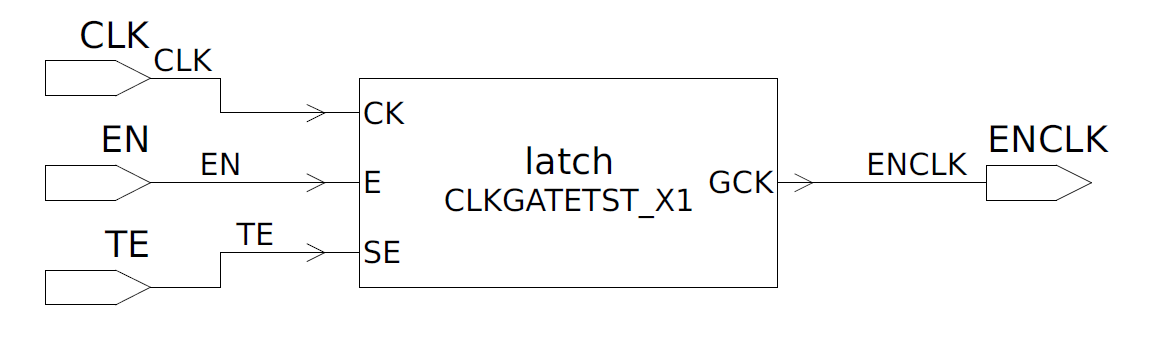
\includegraphics[width=10cm]{./img/Lab_3/clock_gating_implementation.png}}
\\\\       
Si nota che non è presente alcuna struttura adibita al clock gating sul registro in uscita; infatti, dalla descrizione VHDL, il sintetizzatore non è in grado di riconoscere la possibilità di applicare il clock gating. A tal proposito, il codice è stato modificato al fine di includere questa opzione.
\begin{center}
\begin{listato}
	\centerline{\lstinputlisting{./code/Lab_3/clock_gating_output.vhd}}
\end{listato}
\end{center}
In particolare, è stato notato che all'interno del process per la descrizione dell'architettura, l'aggiornamento dei registri REG\_A e REG\_B avviene successivamente a due condizioni di if relative al valore di INCA e INCB. Si ipotizza che, tramite tale descrizione, il sintetizzatore sia in grado di applicare il clock gating. Di conseguenza, tale sintassi è stata adottata anche per descrivere l'aggiornamento del registro in uscita, il quale deve essere aggiornato solo quando almeno un segnale di incremento viene asserito.
\\\\
Nelle seguenti tabelle sono riportati i risultati relativi ai consumi.      
\begin{center}
	\begin{tabular}{|c|c|c|c|c|}
	\hline
	\multicolumn{3}{|c|}{Power report - statistiche di default}\\
	\hline
	& No clock gating & Clock gating \\
	\hline
	Internal power [uW] & 39.1897 & 33.1194 \\
	\hline
	Net switching power [uW] & 14.8742  & 10.8040 \\
	\hline
	Leakage power [uW] & 4.6358 & 4.0346 \\
	\hline
	Total power [uW] & 58.6997 & 47.9580 \\
	\hline
	\end{tabular}	
\end{center}
\vspace{0.3cm}      
\begin{center}
	\begin{tabular}{|c|c|c|}
	\hline
	\multicolumn{3}{|c|}{Power report - reset modificato}\\
	\hline
	& No clock gating & Clock gating \\
	\hline
	Internal power [uW] & 28.3881 & 27.8883 \\
	\hline 
 	Net switching power [uW] & 16.4611 & 11.9228 \\
	\hline
	Leakage power [uW] & 4.6611 & 4.4199 \\
	\hline
	Total power [uW] & 49.5103 & 44.2311 \\
	\hline
	\end{tabular}	
\end{center}
\vspace{0.3cm}    
\begin{center}
	\begin{tabular}{|c|c|c|}
	\hline
	\multicolumn{3}{|c|}{Power report - reset e ingressi modificati}\\
	\hline
	& No clock gating & Clock gating \\
	\hline
	Internal power [uW] & 21.3760 & 10.0773 \\
	\hline 
 	Net switching power [uW] & 11.4117 & 4.1839 \\
	\hline
	Leakage power [uW] & 4.5424 & 4.3468 \\
	\hline
	Total power [uW] & 37.3300 & 18.6080 \\
	\hline
	\end{tabular}	
\end{center}
\vspace{0.3cm}          
Si nota che il clock gating porta ad una riduzione generale della potenza, che risulta più marcata se si considerano statistiche realistiche degli input e del seganle di reset, come già verificato in precedenza. Tuttavia, applicando tale tecnica, la potenza di leakage presenta una riduzione: si ipotizza che tale comportamento inatteso sia correlato ad una riduzione delle celle utilizzate.
\\
Per verificare ciò è stato effettuato un report di tipo \textbf{-cell}.
\\
\begin{center}
	\begin{tabular}{|c|c|c|}
	\hline
	\multicolumn{3}{|c|}{Cell report - reset e ingressi modificati}\\
	\hline
	& No clock gating & Clock gating \\
	\hline
	Numero celle & 96 & 81 \\
	\hline
	 Area [um$^2$] & 244.72 & 243.66 \\
	\hline
	\end{tabular}	
\end{center}
\vspace{0.3cm} 
 L'ipotesi di riduzione del numero di celle è confermata, tuttavia tale risultato è in controtendenza con quanto atteso successivamente all'implementazione di clock gating: ci si aspetta un incremento dell'area totale dovuto all'inserimento della logica atta all'implementazione di tale tecnica.
 \\\\
Si ipotizza che, a causa della modifica apportata al file VHDL, il sintetizzatore, nel caso in cui non sia specificato di applicare il clock gating, interpreti la descrizione inserendo della logica aggiuntiva per verificare la condizione di if. Al contrario, applicando la direttiva \textbf{-gate\_clock}, la descrizione viene interpretata correttamente dal sintetizzatore.
\\
Il numero di celle risulta comunque maggiore rispetto al caso in cui il clock gating viene applicato solamente ai registri REG\_A e REG\_B.
\\
\subsection{Simulazione di consumi tramite back-annotation}
Al fine di ottenere una stima più accurata del consumo di potenza del circuito preso in considerazione, è necessario avere una valutazione più realistica dell'attività dei singoli nodi del circuito sintetizzato. A tale scopo è possibile effettuare una simulazione back-annotated, generando post-sintesi un file SDF contenente la descrizione della netlist del circuito.
\\
L'ambiente di simulazione ModelSim è in grado, partendo dal file di cui sopra, di svolgere diverse simulazioni atte a caratterizzare l'attività dei nodi in questione. Tali risultati vengono riportati in un apposito file VCD che, successivamente ad una conversione in un file SAIF, può essere letto dal CAD di sintesi.
\\
Attraverso le informazioni ottenute, si è in grado di simulare più realisticamente il comportamento del circuito in termini di potenza. Sono riportati di seguito i risultati.
\\\\
\begin{center}
	\begin{tabular}{|c|c|c|c|}
	\hline
	Internal power [uW] & Net switching power [uW] & Leakage power [uW] & Total power [uW] \\
	\hline
	 39.6187 & 18.3103  & 4.6799  &  62.6089 \\
	\hline
	\end{tabular}	
\end{center}
\vspace{0.3cm}
\begin{center}
	\begin{tabular}{|c|c|c|}
	\hline
Segnale & Static probability & Toggle rate \\
	\hline
	 clock & 0.5  &  0.4 \\
	\hline
	 reset & 0.004  &  0.0005 \\
	\hline
	 INCA & 0.019  &  0.001 \\
	\hline
	 INCB & 0.986  &  0.0005 \\
	\hline
	\end{tabular}	
\end{center}
\vspace{0.3cm}
È possibile notare che i valori di static probability e toggle rate sono differenti rispetto a quanto impostato precedentemente su Synopsys. In particolare, l'ingresso INCB ha una probabilità prossima a 1 e una switching acitivity molto bassa.
\\
Si ipotizza che i consumi elevati siano dovuti al quasi continuo incremento del valore contenuto nel registro REG\_B. Tale fatto mette in luce l'importanza di un testbench in grado di rappresentare correttamente la statistica  degli input del circuito.
\newpage
\section{Pipelining e parallelizzazione}
Al fine di ridurre il consumo di potenza dinamica di un generico circuito che presenta un datapath delimitato da barriere di registri, è possibile applicare una serie di soluzioni architetturali.
\\\\
In particolare, è preso in considerazione il medesimo circuito usato nei punti precedenti, il quale è stato caratterizzato dal punto di vista di ritardo, potenza e area.
Le condizioni di funzionamento standard consistono in V\textsubscript{dd} = 1V e f\textsubscript{clk} = 5MHz.
\begin{itemize}
\item percorso critico = reg + inc + comp + mux = 140 ns
\item frequenza massima = 7.14MHz
\item potenza @ 5MHz = 3 reg + 2 inc + comp + mux = 10.73 uW
\item area = 3 reg + 2 inc + comp + mux = 1747 um$^2$
\end{itemize}
\vspace{0.3cm}
È possibile apportare dei miglioramenti in termini di consumo di potenza adottando svariate tecniche a livello architetturale: una di queste consiste nella parallelizzazione del datapath come mostrato nella seguente figura.
\\\\
\centerline{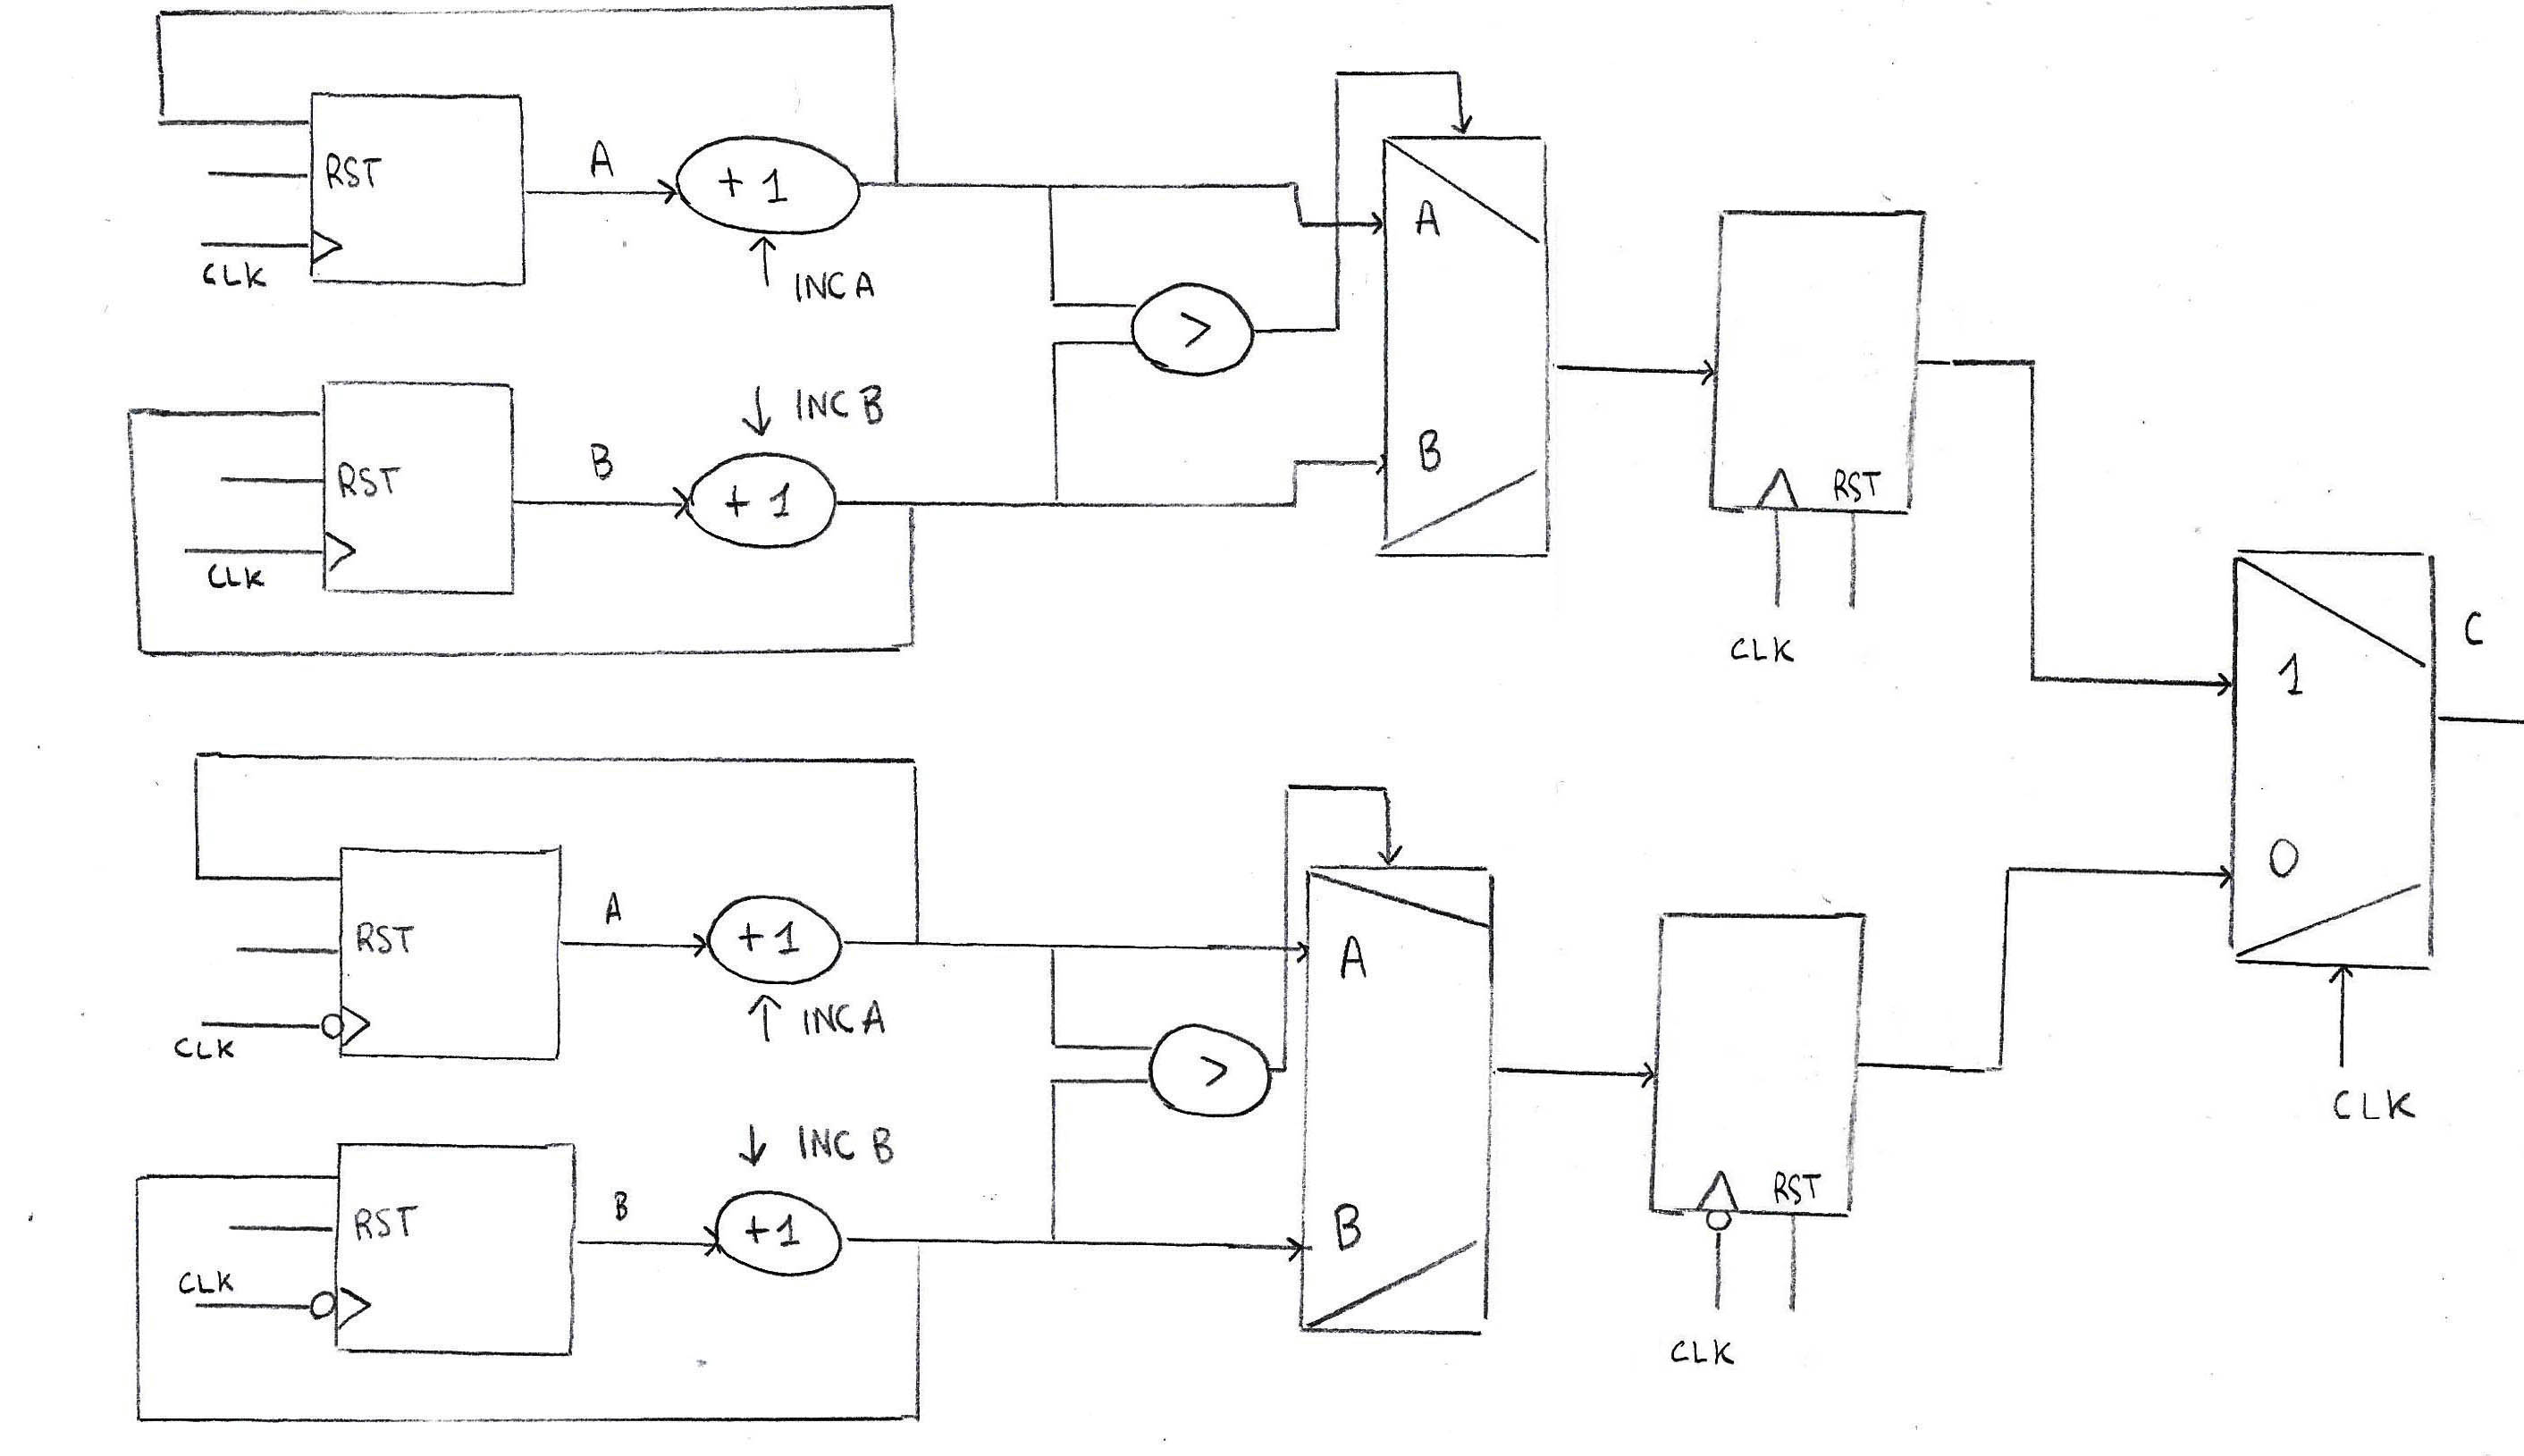
\includegraphics[width=10cm]{./img/Lab_3/datapath_parallelo.jpg}}
\\\\
In particolare, duplicando il datapath e inserendo un opportuno multiplexer, è possibile far lavorare i componenti a metà della frequenza originale, mantenendo comunque lo stesso throughput in uscita del circuito di partenza. Data l'espressione per valutare il consumo di potenza dinamica:
\\\\
\centerline{P = C\textsubscript{eff} V\textsubscript{dd}$^2$ f\textsubscript{clk}}
\\\\
è possibile notare come, in questo caso, il dimezzamento della frequenza di funzionamento sia compensato dal raddoppio della capacità totale.
\\
Tuttavia, i componenti hanno il doppio del tempo a disposizione per completare le loro operazioni, pertanto è possibile ridurre la tensione di alimentazione al fine di aumentare il ritardo di propagazione in questi ultimi, rispettando comunque il limite imposto dal percorso critico.
\\\\
Dal momento che la tensione di alimentazione contribuisce in modo quadratico al consumo di potenza, quest'ultima risulterà ridotta di un fattore u$^2$, dove u rappresenta il fattore di riduzione di V\textsubscript{dd}.
\\\\
\centerline{P(u) = P\textsubscript{nom} u$^2$}
\\\\
I ritardi di propagazione non si riducono linearmente con la tensione di alimentazione ma seguono un andamento che può essere descritto dalla seguente formula:
\\\\
\centerline{$T(u) = T\textsubscript{nom} \frac{0.75u}{u-0.25}$}
\\\\
Il seguente grafico mostra, in unità relative, l'andamento di potenza e ritardo in funzione del fattore di scalamento.
\\\\
\centerline{\includegraphics[width=10cm]{./img/Lab_3/grafico_u.png}}
\\\\
La modifica apportata all'architettura consente, come mostrato in precedenza, di lavorare ad una frequenza pari alla metà della frequenza nominale, di conseguenza si stima che i ritardi non possano essere incrementati al di sopra di un fattore 2.
\\
Considerando ciò e osservando il grafico è stato scelto u = 0.5, corrispondente ad un buon trade-off tra riduzione dei consumi e aumento dei ritardi. Successivamente è stata caratterizzata nuovamente la tabella che descrive i parametri dei componenti.
\\\\
\begin{center}
	\begin{tabular}{|c|c|c|c|}
	\hline
	Cella & Ritardo [ns] & Potenza @2.5MHz [uW] & Area [um$^2$] \\
	\hline
	 registro & 3 & 0.075 & 319 \\
	\hline
	 incrementatore & 60 & 0.319 & 256 \\
	\hline
	 comparatore & 126 & 0.27 & 161 \\
	\hline
	 mux & 21 & 0.209 & 117 \\
	\hline
	\end{tabular}	
\end{center}
\vspace{0.3cm}
Come atteso, si nota che un aumento dei ritardi dei singoli componenti corrisponde ad una riduzione dei loro consumi.
\begin{itemize}
\item percorso critico = reg + inc + comp + mux = 210 ns
\item frequenza massima = 4.76 MHz
\item potenza @ 2.5 MHz = 2$\cdot$(3 reg + 2 inc + comp + mux) + mux(overhead) = 2.89 uW
\item area = 2$\cdot$(3 reg + 2 inc + comp + mux) + mux = 3611 um$^2$
\end{itemize}
\vspace{0.3cm}
Si può notare che la potenza è stata ridotta di un fattore 3.71 a fronte di un raddoppio dell'area. In particolare, è possibile osservare l'effetto dell'overhead del mux in uscita nella valutazione del percorso critico, che risulta maggiore.
\\\\
Un'altra tecnica a livello architetturale applicabile in questo contesto è la pipeline. L'inserimento di registri all'interno del percorso combinatorio permette di ridurre il percorso critico, mantenendo comunque un throughput elevato.
\\
Riducendo il percorso critico si potrebbe lavorare ad una frequenza maggiore rispetto alla frequenza nominale, tuttavia si decide di mantenere lo stesso throughput del circuito originale, avendo quindi la possibilità di incrementare i ritardi attraverso una riduzione di V\textsubscript{dd}.
\\\\
In questo caso si è deciso di isolare, attraverso due barriere di registri, il comparatore, essendo il componente che presenta il maggior ritardo di propagazione. Di conseguenza è stato ottenuto il seguente datapath.
\\\\
\centerline{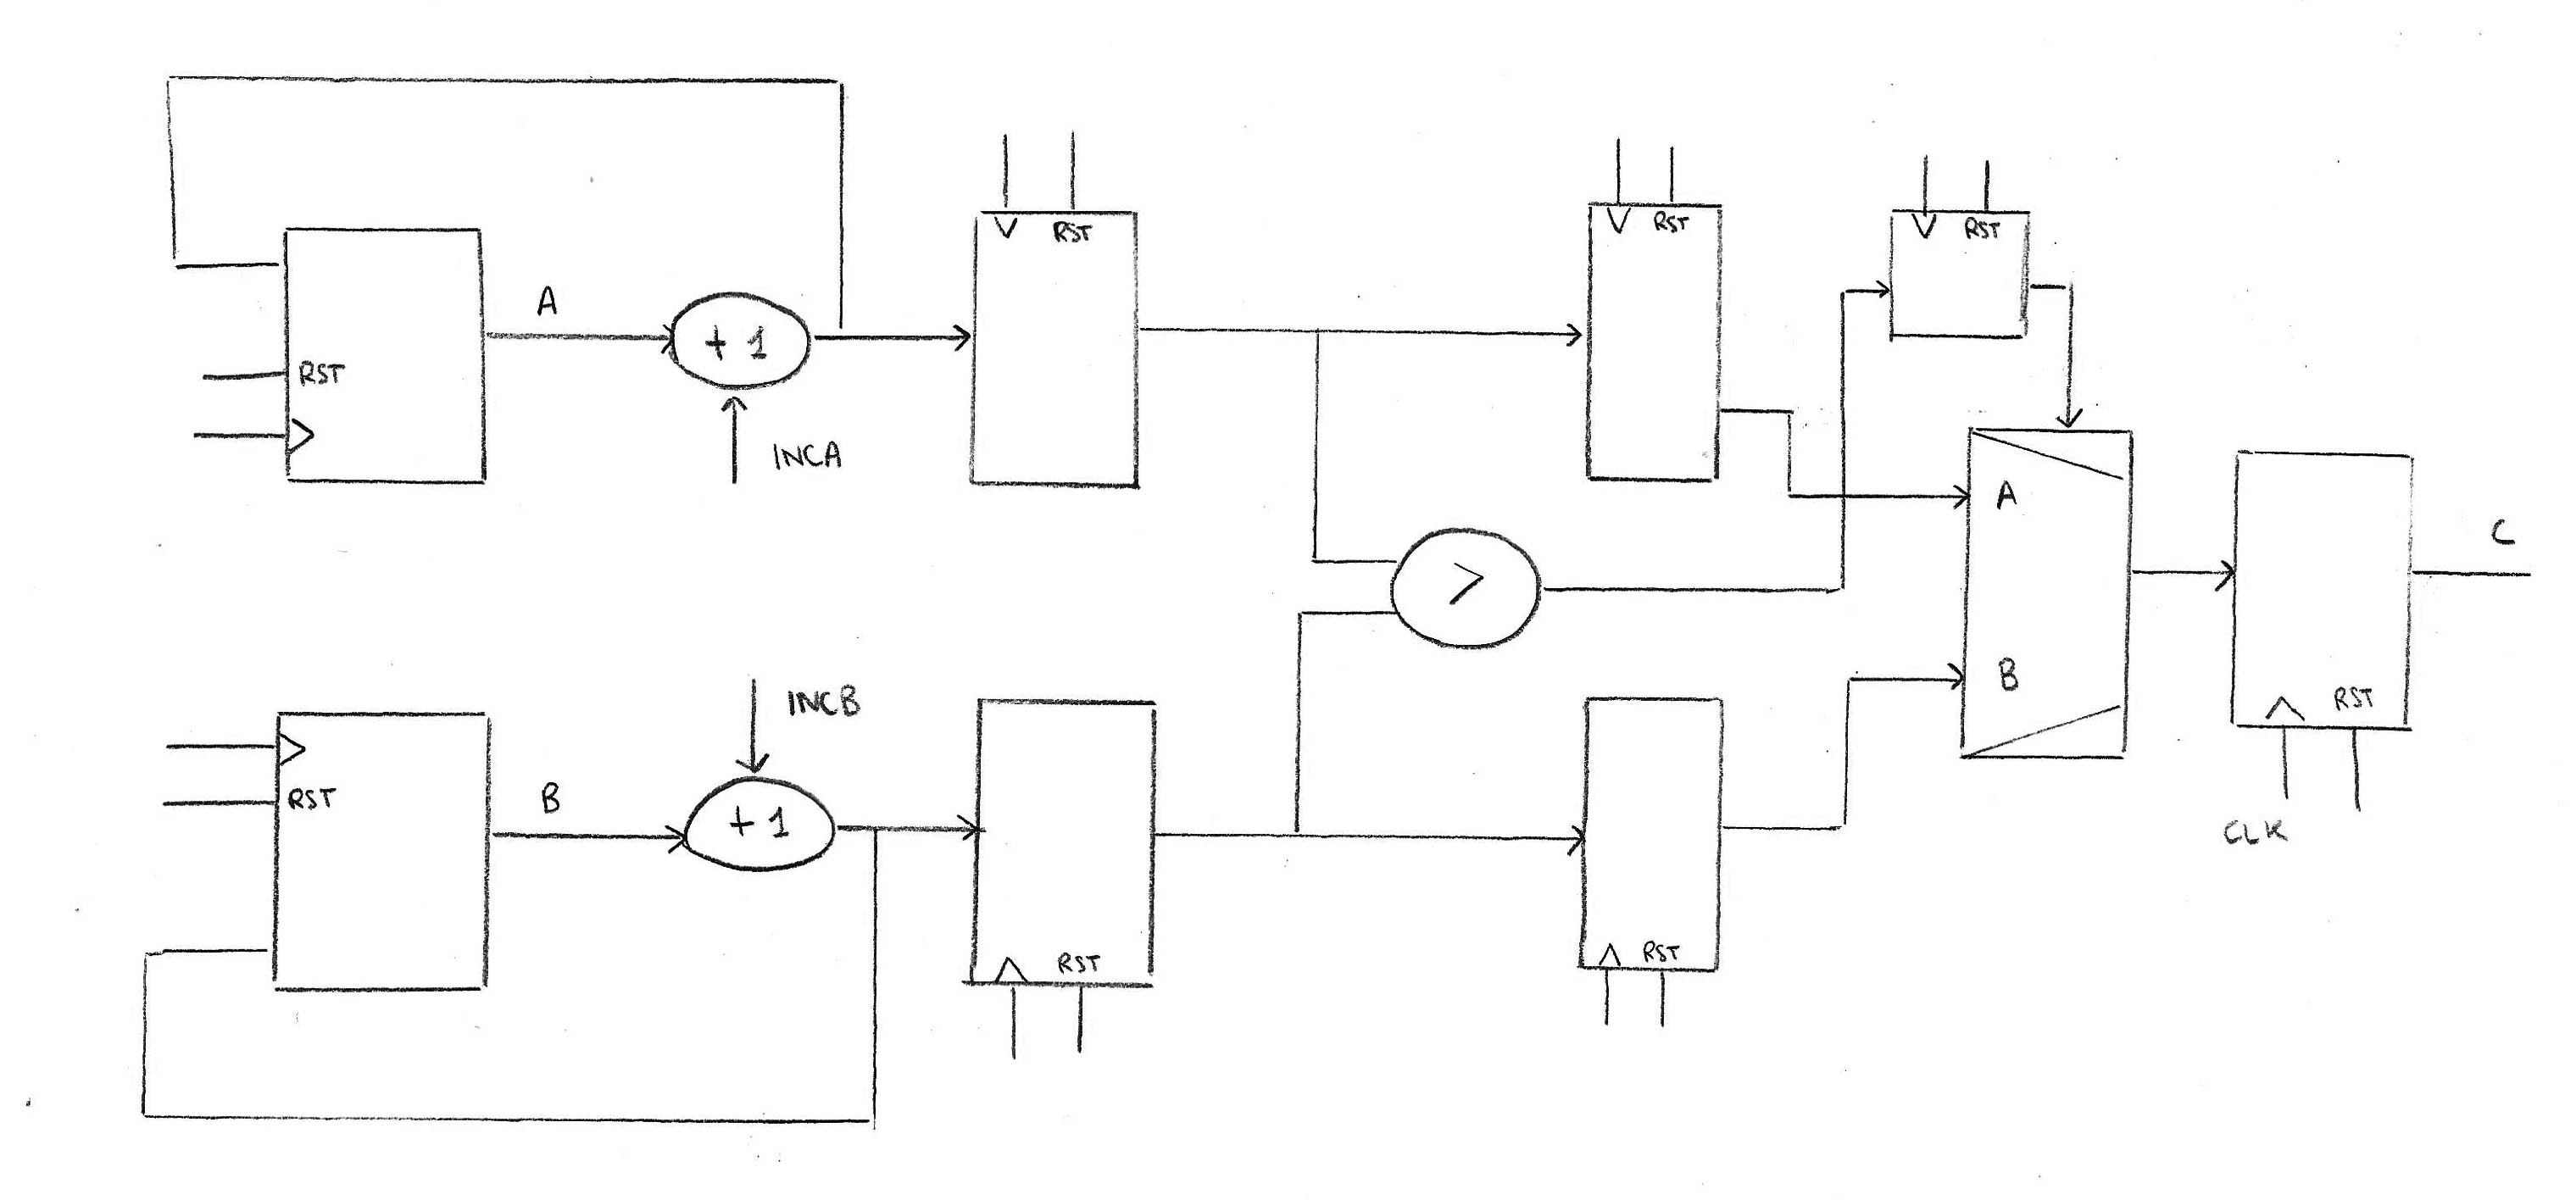
\includegraphics[width=10cm]{./img/Lab_3/datapath_pipeline.jpeg}}
\\\\
Si fa presente che per garantire la coerenza è necessario inserire elementi di memoria in modo da assicurare il corretto timing di dati e controlli.
È dunque possibile stimare il nuovo percorso critico del circuito, considerando la tensione di alimentazione nominale:
\\\\
\centerline{percorso critico: 1 reg + 1 comp = 86 ns}
\\\\
tale valore consente di lavorare ad una massima frequenza pari  a 11.63 MHz. Date le considerazioni precedenti, nel contesto attuale è sufficiente lavorare ad una frequenza di 5 MHz, pari a quella nominale.
\\
Il massimo fattore di scalamento dei ritardi di propagazione è pari a:
\\\\
\centerline{$\frac{11.63}{5}$ = 2.33}
\\\\
A tale fattore di scalamento corrisponde una u\textsubscript{max} = 0.37, ricavata invertendo la formula precedentemente riportata. In questo caso, è stata ricercata la massima riduzione possibile della tensione di alimentazione.
\\\\
\begin{center}
	\begin{tabular}{|c|c|c|c|}
	\hline
	Cella & Ritardo [ns] & Potenza @5MHz [uW] & Area [um$^2$] \\
	\hline
	 registro & 4.6 & 0.082 & 319 \\
	\hline
	 incrementatore & 92.5 & 0.349 & 256 \\
	\hline
	 comparatore & 194.25 & 0.296 & 161 \\
	\hline
	 mux & 32.4 & 0.228 & 117 \\
	\hline
	\end{tabular}	
\end{center}
\begin{itemize}
\item percorso critico = reg +  comp = 198.85 ns
\item frequenza massima = 5.03 MHz
\item potenza @ 5 MHz = 3 reg + 2 inc + comp + mux + 5 reg (pipe) = 1.86 uW
\item area = 3 reg + 2 inc + comp + mux + 5 reg (pipe) = 3342 um$^2$
\end{itemize}
\vspace{0.3cm}
Come atteso, si nota una significativa riduzione del consumo di potenza, pari ad un fattore 5.77. Inoltre, il circuito risulta più compatto rispetto al caso della parallelizzazione.
\\\\
In generale, la tecnica della pipeline permette di raggiungere risultati migliori in termini di trade-off tra potenza e area. Tuttavia tale soluzione modifica radicalmente il timing del sistema, il quale rimane invariato nel caso di utilizzo della tecnica di parallelizzazione.
\\\\
Di conseguenza, la tecnica migliore dipende fortemente dal contesto di progetto: nel caso di un sistema da progettare si privilegia la pipeline; al contrario, nel caso sia necessaria un'ottimizzazione di un sistema già progettato è prediletta la tecnica della parallelizzazione in quanto meno invasiva.
\\\\
Per confronto si è cercato il minimo consumo di potenza applicando solamente la tecnica della parallelizzazione, con parallelismo 2.  In seguito alla riduzione di V\textsubscript{dd}, il minimo consumo di potenza dinamica ottenibile è pari a 1.85 uW, scegliendo u = 0.4, consumo comparabile a quello ottenuto con la tecnica di pipeline.
\\
Per raggiungere un'ulteriore riduzione dei consumi, è necessario introdurre un terzo livello di parallelizzazione: in questo caso è possibile selezionare u = 0.37, ottenendo quindi un consumo di potenza pari a 1.58 uW.
\\\\
Partendo dalla soluzione parallelizzata, sono stati ricercati possibili miglioramenti unendo le due tecniche. Il grafico seguente mostra il prodotto potenza ritardo in funzione del fattore u, considerando la presenza di pipeline e di un parallelismo pari a 2.
\\\\
\centerline{\includegraphics[width=12cm]{./img/Lab_3/prodotto_potenza_ritardo.png}}
\\\\
Si evince che sarebbe possibile utilizzare un fattore di scalamento della tensione di alimentazione inferiore a 0.37, tuttavia riducendolo vi è un'inversione di tendenza della curva mostrata. Ciò significa che per valori di u al di sotto del punto di minimo, il guadagno in termini di potenza risparmiata è poco significativo rispetto ai ritardi introdotti.
\\
Nonostante l'uso contemporaneo delle due tecniche, l'uso di 3 livelli di sola parallelizzazione risulta la scelta migliore dal punto di vista della sola riduzione dei consumi dinamici.
\\\\
Si fa presente che l'analisi effettuata è relativa alla sola potenza dinamica, infatti una riduzione significativa di V\textsubscript{dd} comporta l'utilizzo di transistor caratterizzati da una tensione di soglia minore, aumentando il contributo di corrente di leakage.
\\\\
Inoltre, la parallelizzazione comporta un overhead elevato in termini di elementi utilizzati, che ha come diretta conseguenza un incremento della potenza di leakage complessiva. Ne consegue che la valutazione della scelta dell'architettura che ottimizza la potenza complessiva debba essere fatta in funzione di contributi sia statici sia dinamici.
\subsection{Il problema della coerenza}
Applicando la tecnica della parallelizzazione all struttura di base, è possibile notare che la coerenza dei dati in uscita non è assicurata.
\\
Considerando le forme d'onda in ingresso come mostrato nella figura seguente, è possibile stimare l'andamento atteso dell'uscita C nel caso del circuito originale.
\\\\
\centerline{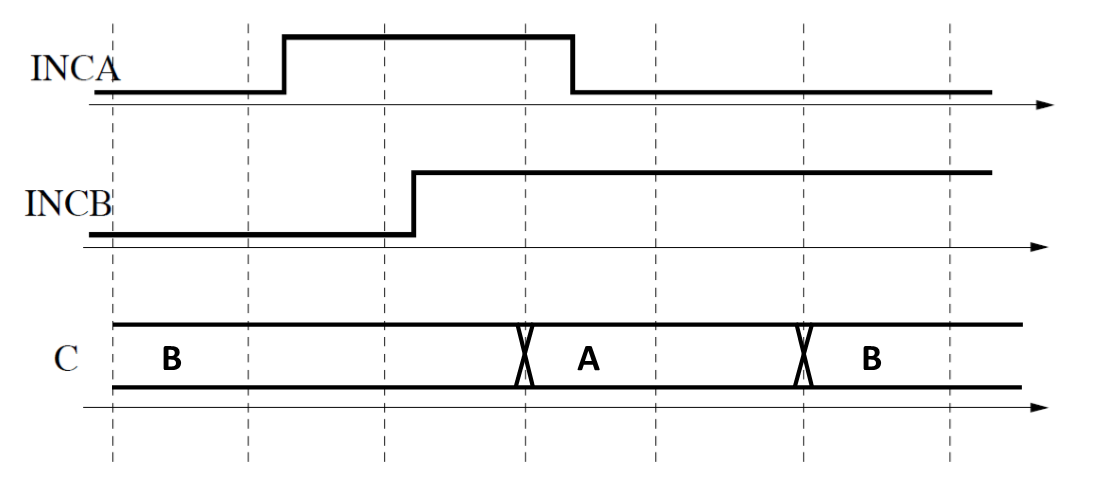
\includegraphics[width=12cm]{./img/Lab_3/Comportamento_atteso.png}}
\\\\
Al contrario nel caso di implementazione con 2 livelli di parallelizzazione si ha il comportamento seguente.
\\\\
\centerline{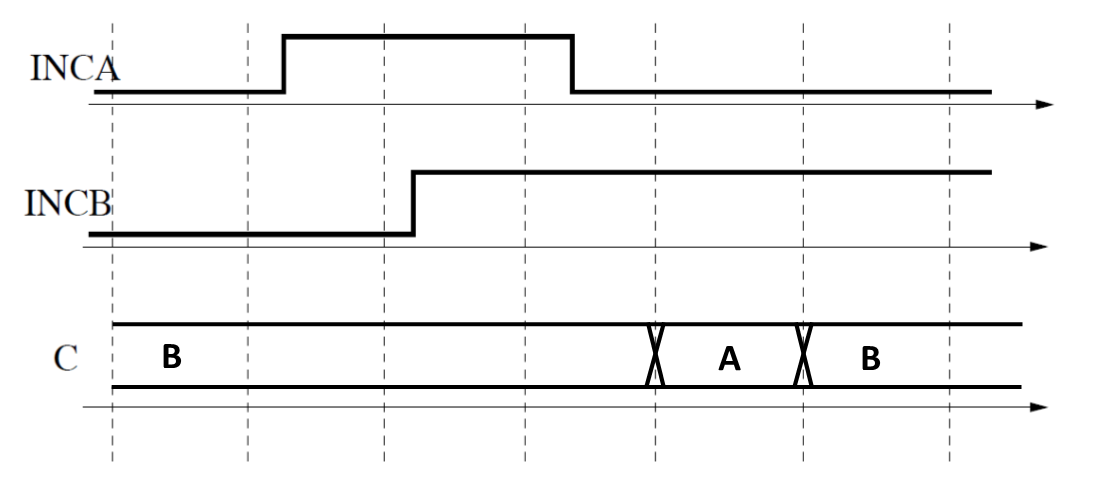
\includegraphics[width=12cm]{./img/Lab_3/Comportamento_attuale.png}}
\\\\
Si nota che il comportamento è inatteso in quanto non vi è coerenza tra i registri delle due sottostrutture. Per assicurare un corretto funzionamento del circuito, è necessario che i dati con cui lavorano le due entità siano condivisi, in modo da garantire la coerenza.
\\\\
Una possibile soluzione potrebbe essere l'impiego di due soli registri REG\_A e REG\_B condivisi da entrambe le strutture in parallelo e scritti ad una frequenza doppia.

\chapter{Bus encoding}
\section{Introduzione alle tecniche utilizzate}
Lo scopo di questa esercitazione è testare diverse codifiche utilizzate per ridurre le commutazioni sui bus. È fondamentale, in un contesto low power, prestare attenzione ai consumi relativi alle interconnessioni, in quanto ad esse è associata una capacità significativa.
\\\\
In particolare, sono state testate le seguenti tecniche:
\begin{itemize}
\item \textbf{Bus normale}
\\
Interconnessione priva di qualunque tipo di codifica e, per tale motivo, non ridondante.
\item \textbf{Bus invert}
\\
Il valore logico sull'interconnesione è invertito se la distanza di Hamming rispetto al valore precedente è maggiore di $\frac{N}{2}$, dove N è il parallelismo dell'informazione. Si tratta di una codifica ridondante, infatti è necessario notificare al ricevitore l'eventuale inversione dell'informazione inviata.
Tale codifica è idonea alla trasmissione dei dati, in quanto la statistica di questi è casuale rispetto a quella di indirizzi e controlli.
\item \textbf{Transition based}
\\
L'informazione è codificata non attraverso un livello logico ma con una transizione della linea, che avviene quando il dato assume un valore pari a 1. Si nota che tale codifica non è ridondante dal momento che non sono necessari ulteriori segnali.
\\
I circuiti di codifica e decodifica fanno uso di porte XOR e flip flop per memorizzare il valore precedente, che viene comparato con quello attuale. Si nota che, in trasmissione, un valore di A pari a 1 porta alla commutazione del bus rispetto al valore assunto precedentemente. In ricezione, invece, quando è identificata una transizione sul bus, confrontando il valore attuale con quello precedente, l'uscita C assume un valore logico alto.
\\\\
\centerline{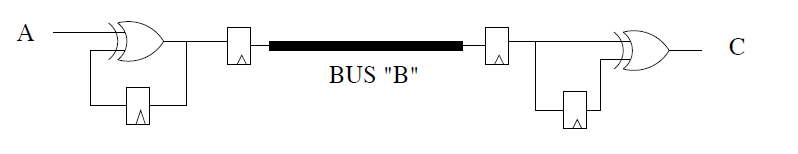
\includegraphics[width=12cm]{./img/Lab_4/tran_based.png}}
\\\\
\item \textbf{Gray code}
\\
La codifica ha come principale scopo il mantenimento della distanza di Hamming pari a 1 tra due informazioni consecutive. Tale codifica risulta appropriata per la trasmissione degli indirizzi. Si nota inoltre che questa codifica non prevede l'invio di ulteriori segnali di controllo, è pertanto non ridondante.
\\
In particolare, il seguente schema mostra i circuiti di codifica e decodifica.
\\\\
\centerline{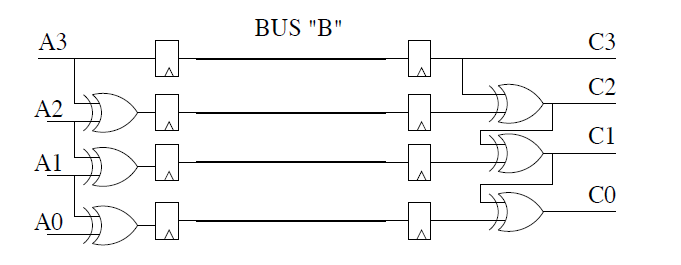
\includegraphics[width=12cm]{./img/Lab_4/gray.png}}
\\\\
È possibile notare come un ingresso sia codificato correttamente solo andando in sequenza.
\item \textbf{T0 encoding}
\\
Tale codifica ha il principale scopo di eliminare le commutazioni sul bus, nel caso in cui l'informazione sia sequenziale: per tale motivo è particolarmente adatta alla trasmissione indirizzi. Quando è identificata una sequenza dal trasmettitore, quest'ultimo mantiene l'indirizzo di partenza fisso sul bus e abilita un apposito segnale aggiuntivo atto a segnalare al ricevitore la sequenzialità dell'informazione.
\\
Per tale motivo è necessario implementare un incrementatore al ricevitore per generare l'indirizzo corretto.
\\
In caso di salto, quest'ultimo viene segnalato cambiando l'indirizzo inviato sul bus e negando il segnale seq.
Si nota quindi che tale tecnica è ridondante.
\\\\
\textcolor{red}{Possibile schema a blocchi, se non serve rimuovere l'immagine sotto}
\\\\
\centerline{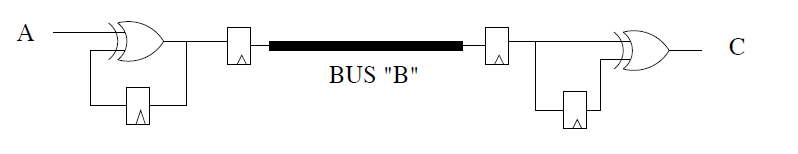
\includegraphics[width=12cm]{./img/Lab_4/tran_based.png}}
\\\\
Basandosi sul principio di funzionamento sopra descritto, è stata realizzata la seguente descrizione VHDL.
\begin{center}
\begin{listato}
	\centerline{\lstinputlisting{./code/Lab_4/T0beh.vhd}}
\end{listato}
\end{center}
\end{itemize}
\section{Simulazione}
Attraverso la piattaforma ModelSim è possibile, tramite un testbench, ottenere una stima dell'attività relativa alle diverse tecniche di codifica implementate.
\\
Dal momento che alcune codifiche sono più appropriate al trattamento di dati o indirizzi, vi è la possibilità di generare sequenze di informazioni con opportune distribuzioni statistiche.
\\\\
All'interno del file \textbf{tb\_encdec.v} è possibile, attraverso due direttive, scegliere la statistica dei segnali da simulare, opportunamente generata tramite due process. In particolare, si nota come il process relativo ai dati prelevi questi ultimi dal file \textbf{rdin.txt} dove è presente una sequenza pseudo-random di valori rappresentati su 8 bit.
\\\\
Al contrario, il process atto alla generazione degli indirizzi, procede in sequenza fino al raggiungimento dell'indirizzo 63, successivamente al quale simula un salto prelevando l'indirizzo successivo dal file di cui sopra.
\\
Tutte le tecniche di codifica sono state simulate sia con dati che con indirizzi, riportando le attività dell'ingresso A e delle linee di bus B. Come primo risultato, è interessante notare la diversa attività delle due statistiche dell'informazione in ingresso.
\\\\
\begin{center}
	\begin{tabular}{|c|c|c||c|c|}
	\hline
	& \multicolumn{2}{|c||}{Address} & \multicolumn{2}{|c|}{Data}\\
	\hline
	Nodo & Tc & E\textsubscript{sw} & Tc & E\textsubscript{sw} \\
	\hline
	 A(7) & 97 & 0.0097 & 4974 & 0.4974\\
	 \hline
	A(6) & 118 & 0.0118 & 5022 & 0.5022\\
	\hline
	A(5) & 312 & 0.0312 & 4987 & 0.4987\\
	\hline
	A(4) & 625 & 0.0625 & 4972 & 0.4972\\
	\hline
	A(3) & 1250 & 0.1250 & 4960 & 0.4960\\
	\hline
	A(2) & 2500 & 0.2500 & 4965 & 0.4965\\
	\hline
	A(1) & 5000 & 0.5000 & 5024 & 0.5024\\
	\hline
	A(0) & 10000 & 1 & 5060 & 0.5060\\
	\hline
	Totale & 19902 & 1.9902 & 39964 & 3.9964\\
	\hline
	\end{tabular}	
\end{center}
\vspace{0.3cm}
Come atteso, la statistica relativa ai dati presenta attività maggiori e confrontabili tra loro. Per quanto riguarda gli indirizzi, invece, si nota un'attività che mostra la sequenzialità.
\subsection{Bus normal}
\begin{center}
	\begin{tabular}{|c|c|c||c|c|}
	\hline
	& \multicolumn{2}{|c||}{Address} & \multicolumn{2}{|c|}{Data}\\
	\hline
	Nodo & Tc & E\textsubscript{sw} & Tc & E\textsubscript{sw} \\
	\hline
	 BUSNORM(7) & 97 & 0.0097 & 4974 & 0.4974\\
	 \hline
	BUSNORM(6) & 118 & 0.0118 & 5021 & 0.5021\\
	\hline
	BUSNORM(5) & 312 & 0.0312 & 4987 & 0.4987\\
	\hline
	BUSNORM(4) & 624 & 0.0624 & 4972 & 0.4972\\
	\hline
	BUSNORM(3) & 1249 & 0.1249 & 4959 & 0.4959\\
	\hline
	BUSNORM(2) & 2499 & 0.2499 & 4965 & 0.4965\\
	\hline
	BUSNORM(1) & 4999 & 0.4999 & 5023 & 0.5023\\
	\hline
	BUSNORM(0) & 9999 & 0.9999 & 5060 & 0.5060\\
	\hline
	Totale & 19897 & 1.9897 & 39961 & 3.9961\\
	\hline
	\end{tabular}	
\end{center}
\vspace{0.3cm}
Come atteso, in assenza di codifica, l'attività del bus rispecchia quella dell'ingresso.
\subsection{Bus invert}
\begin{center}
	\begin{tabular}{|c|c|c||c|c|}
	\hline
	& \multicolumn{2}{c}{Address} & \multicolumn{2}{c}{Data}\\
	\hline
	Nodo & Tc & E\textsubscript{sw} & Tc & E\textsubscript{sw} \\
	\hline
	inv & 624 & 0.0624 & 3650 & 0.3650\\
	\hline
	BUSINV(7) & 527 & 0.0527 & 3576 & 0.3576\\
	 \hline
	BUSINV(6) & 506 & 0.0506 & 3611 & 0.3611\\
	\hline
	BUSINV(5) & 312 & 0.0312 & 3617 & 0.3617\\
	\hline
	BUSINV(4) & 0 & 0 & 3640 & 0.3640\\
	\hline
	BUSINV(3) & 625 & 0.0625 & 3613 & 0.3613\\
	\hline
	BUSINV(2) & 1875 & 0.1875 & 3601 & 0.3601\\
	\hline
	BUSINV(1) & 4375 & 0.4375 & 3639 & 0.3639\\
	\hline
	BUSINV(0) & 9375 & 0.9375 & 3722 & 0.3722\\
	\hline
	Totale & 18219 & 1.8219 & 32669 & 3.2669\\
	\hline
	\end{tabular}	
\end{center}
\vspace{0.3cm}
Come atteso, osservando i valori totali, è possibile notare come sia presente una significativa riduzione delle commutazioni per quanto riguarda i dati rispetto al bus normal. Al contrario, le attività degli indirizzi risultano confrontabili.
\\
La riduzione delle commutazioni è tanto più marcata quante più transizioni con una distanza di Hamming maggiore di 4 sono presenti nei dati; attraverso uno script Matlab è stata stimata la percentuale di tali transizioni sul totale, che risulta pari a circa il 36\%.
\subsection{Transition based}
\begin{center}
	\begin{tabular}{|c|c|c||c|c|}
	\hline
	& \multicolumn{2}{|c||}{Address} & \multicolumn{2}{|c|}{Data}\\
	\hline
	Nodo & Tc & E\textsubscript{sw} & Tc & E\textsubscript{sw} \\
	\hline
	TRAN(7) & 4816 & 0.4816 & 5003 & 0.5003\\
	 \hline
	TRAN(6) & 3776 & 0.3776 & 4946 & 0.4946\\
	\hline
	TRAN(5) & 4992 & 0.4992 & 4938 & 0.4938\\
	\hline
	TRAN(4) & 4992 & 0.4992 & 4997 & 0.4997\\
	\hline
	TRAN(3) & 5000 & 0.5000 & 5125 & 0.5125\\
	\hline
	TRAN(2) & 5000 & 0.5000 & 4989 & 0.4989\\
	\hline
	TRAN(1) & 5000 & 0.5000 & 5000 &0.5000 \\
	\hline
	TRAN(0) & 5000 & 0.5000 & 4994 & 0.4994\\
	\hline
	Totale & 38576 & 3.8576 & 39992 & 3.9992\\
	\hline
	\end{tabular}	
\end{center}
\vspace{0.3cm}
Si nota come tale codifica non sia indicata per gli indirizzi in quanto la sequenza stessa ha come prerogativa il mantenimento di valori logici alti sulle linee di bus.
\\
Per quanto riguarda i dati, è atteso un miglioramento nel caso in cui la probabilità di avere valori logici alti sia sufficientemente ridotta. Tuttavia, analizzando il file \textbf{rndin.txt} è possibile osservare la presenza di numerosi 1 all'interno dei dati.
\subsection{Gray coding}
\begin{center}
	\begin{tabular}{|c|c|c||c|c|}
	\hline
	& \multicolumn{2}{|c||}{Address} & \multicolumn{2}{|c|}{Data}\\
	\hline
	Nodo & Tc & E\textsubscript{sw} & Tc & E\textsubscript{sw} \\
	\hline
	GRAY(7) & 97 & 0.0097 & 4974 & 0.4974\\
	 \hline
	GRAY(6) & 55 & 0.0055 & 5087 & 0.5087\\
	\hline
	GRAY(5) & 194 & 0.0194 & 4952 & 0.4952\\
	\hline
	GRAY(4) & 312 & 0.0312 & 4981 & 0.4981\\
	\hline
	GRAY(3) & 625 & 0.0625 & 4937 & 0.4937\\
	\hline
	GRAY(2) & 1250 & 0.1250 & 5056 & 0.5056\\
	\hline
	GRAY(1) & 2500 & 0.2500 & 4962 & 0.4962\\
	\hline
	GRAY(0) & 5000 & 0.5000 & 5075 & 0.5075\\
	\hline
	Totale & 10033 & 1.0033 & 40024 & 4.0024\\
	\hline
	\end{tabular}	
\end{center}
\vspace{0.3cm}
Come atteso, tale codifica non ha benefici nel trattare la trasmissione di dati, ma presenta notevoli miglioramenti per quanto riguarda gli indirizzi. L'attività totale degli indirizzi risulta infatti dimezzata rispetto al caso bus normal.
\subsection{T0}
\begin{center}
	\begin{tabular}{|c|c|c||c|c|}
	\hline
	& \multicolumn{2}{|c||}{Address} & \multicolumn{2}{|c|}{Data}\\
	\hline
	Nodo & Tc & E\textsubscript{sw} & Tc & E\textsubscript{sw} \\
	\hline
	seq & 119 & 0.0119 & 72 & 0.0072  \\
	\hline
	T0(7) & 29 & 0.0029 & 4974 & 0.4974\\
	 \hline
	T0(6) & 24 & 0.0024 & 5021 & 0.5021\\
	\hline
	T0(5) & 0 & 0 & 4987 & 0.4987\\
	\hline
	T0(4) & 0 & 0 & 4972 & 0.4972\\
	\hline
	T0(3) & 0 & 0 & 4957 & 0.4957\\
	\hline
	T0(2) & 0 & 0 & 4963 & 0.4963\\
	\hline
	T0(1) & 0 & 0 & 5001 & 0.5001\\
	\hline
	T0(0) & 0 & 0 & 5028 & 0.5028\\
	\hline
	Totale & 172 & 0.0172 & 39975 & 3.9975\\
	\hline
	\end{tabular}	
\end{center}
\vspace{0.3cm}
Si nota un netto miglioramento per la trasmissione degli indirizzi, in particolare l'attività molto bassa mette in luce che gli indirizzi generati mostrano un'elevata sequenzialità.
\\
I dati presentano invece un'elevata attività, rimanendo in linea con i risultati attesi.
\newpage
\section{Sintesi}
Lo scopo di questa sezione è l'analisi del consumo di potenza relativo alle varie tecniche implementate. Tale stima è stata effettuata attraverso il procedimento di back-annotation descritto nel laboratorio precedente, in modo da ottenere stime verosimili sia per dati che per indirizzi.
\\\\
L'intero processo è basato su un insieme di script forniti che descrivono la sequenza delle operazioni da svolgere, coinvolgendo i tool ModelSim e Synopsys. L'analisi è inoltre effettuata considerando diversi carichi capacitivi per le linee di interconnessione.
\\\\
Inizialmente sono stati valutati, per ogni codifica, i contributi di potenza relativi alle sole linee di bus B, riportati nella seguente tabella.
\\\\
\begin{center}
	\begin{tabular}{|c|c|c|c|c||c|c|c|c|}
	\hline
	Power [uW] & \multicolumn{4}{|c||}{Address} & \multicolumn{4}{|c|}{Data}\\
	\hline
	 & 1fF & 10fF & 50fF & 100fF & 1fF & 10fF & 50fF & 100fF \\
	\hline
	BUSNORM & 0.22 & 1.42 & 6.24 & 12.26 & 0.44 & 2.86 & 12.53 & 24.62 \\
	 \hline
	BUSINV & 0.03 & 1.14 & 5.55 & 11.06 & 0.06 & 2.08 & 9.99 & 19.87 \\
	\hline
	TRAN-BASED & 1.05 & 3.38 & 12.72 & 24.49 & 1.09 & 3.51 & 13.20 & 25.30 \\
	\hline
	GRAY & 0.11 & 0.72 & 3.15 & 6.18 & 0.44 & 2.86 & 12.55 & 24.66 \\
	\hline
	T0 & 0.0009 & 0.0033 & 0.0161 & 0.0322 & 0.73 & 2.49 & 12.15 & 24.22 \\
	\hline
	\end{tabular}	
\end{center}
\vspace{0.3cm}
Osservando tali risultati si nota come vi sia un miglioramento teorico dei consumi utilizzando tutte le codifiche fatta eccezione della TRAN-BASED. La causa di tale eccezione è da ricercare nella distribuzione dei dati generati: questi presentano infatti un numero di 1 elevato.
\\\\
Si nota come l'applicazione della codifica BUSINV riduca la potenza dissipata sia per dati che per indirizzi: in quest'ultimo caso i benefici sono particolarmente marcati nel caso di salti frequenti.
\textcolor{red}{SIMO: in quest'ultimo caso i benefici sono particolarmente marcati nel caso di salti con distanza di Hamming maggiore di N/2.}
\\\\
La codifica GRAY introduce notevoli miglioramenti nella trasmissione degli indirizzi, si nota infatti che il consumo di potenza è dimezzato rispetto al caso BUSNORM. Per quanto riguarda i dati non si notano riduzioni nel consumo di potenza.
\\\\
È possibile osservare come la riduzione di potenza dovuta alla codifica T0 sia particolarmente significativa per gli indirizzi. Questo risultato mette in luce la sequenzialità degli indirizzi di test nella simulazione.
\\\\
Nella seguente tabella sono invece riportati i risultati relativi al consumo di potenza totale, considerando anche il contributo degli ingressi per le varie codifiche implementate.
\textcolor{red}{SIMO: Nella seguente tabella sono invece riportati i risultati relativi al consumo di potenza totale, comprendenti il contributo degli ingressi e della logica atta alle operazioni di codifica e decodifica.}

\begin{center}
	\begin{tabular}{|c|c|c|c|c||c|c|c|c|}
	\hline
	Power [uW] & \multicolumn{4}{|c||}{Address} & \multicolumn{4}{|c|}{Data}\\
	\hline
	 & 1fF & 10fF & 50fF & 100fF & 1fF & 10fF & 50fF & 100fF \\
	\hline
	BUSNORM & 14.76 & 15.99 & 20.82 & 28.16 & 19.34 & 21.81 & 31.51 & 45.97 \\
	 \hline
	BUSINV & 33.58 & 35.19 & 39.61 & 46.33 & 44.32 & 46.18 & 54.10 & 65.90 \\
	\hline
	TRAN-BASED & 35.57 & 38.04 & 47.54 & 61.52 & 34.80 & 37.33 & 47.14 & 61.62 \\
	\hline
	GRAY & 14.85 & 15.47 & 17.91 & 21.75 & 27.48 & 29.95 & 39.67 & 54.15 \\
	\hline
	T0 & 33.53 & 30.80 & 30.87 & 30.55 & 40.73 & 44.33 & 53.87 & 68.30 \\
	\hline
	\end{tabular}	
\end{center}
\vspace{0.3cm}
È possibile, per ogni implementazione, notare un incremento della potenza dissipata in seguito ad un aumento della capacità di carico del bus.
\\
I report ottenuti mostrano come le diverse codifiche dissipino una potenza di leakage differente. In particolare, quest'ultima è legata alla complessità della logica necessaria all'implementazione della tecnica di encoding. Di conseguenza, è stato notato che la codifica T0 presenta il consumo di potenza statica maggiore a causa della presenza di un elevato numero di gate rispetto alle altre codifiche.
\\\\
Osservando i dati relativi alla tecnica BUSINV, si nota come non vi è alcun miglioramento netto né per dati né per indirizzi. Utilizzando tale codifica è atteso un miglioramento per i consumi relativi alla trasmissione dei dati, ciò non avviene poiché la distribuzione di questi non presenta un numero elevato di transizioni con distanza di Hamming maggiore di $\frac{N}{2}$. Di conseguenza, l'aggiunta della logica di codifica e decodifica non ha un contributo trascurabile.
\\\\
Anche per la codifica TRANSITION-BASED non è rilevato alcun miglioramento. Il motivo principale è sempre da ricercare nella distribuzione dei dati. Questi infatti presentano un numero di 1 significativo, generando una quantità elevata di transizioni.
\\\\
Per quanto la codifica GRAY, è possibile notare un miglioramento riguardante la trasmissione di indirizzi. Tale miglioramento risulta sempre più marcato al crescere della capacità di carico del bus: più questa è elevata, più il consumo relativo alla logica di codifica e decodifica diventa trascurabile.
\\\\
Relativamente alla codifica T0 è possibile notare come, simulando gli indirizzi, il consumo rimanga circa costante. Tale comportamento è dovuto al basso numero di commutazioni che la codifica permette di effettuare sui bus, portando quindi in secondo piano il peso delle capacità di carico. Nonostante ciò, l'overhead dovuto alla logica aggiunta, ha un contributo non trascurabile nei contesti analizzati. È implicito che tale codifica non sia particolarmente adatta alla trasmissione dei dati.
\\\\
In generale, nella scelta di una codifica ottimale è importante tenere in considerazione la capacità di carico del bus e confrontarla con la logica necessaria all'implementazione del bus encoding. Infatti, una tecnica in grado di portare un'elevata riduzione delle commutazioni sul bus potrebbe richiedere un consumo di implementazione significativo tale da compensare il risparmio apportato.
\newpage
\section{Approfondimenti}
Al fine di approfondire il funzionamento per le codifiche BUSINV e TRAN-BASED, è stato modificato il file contenente la sequenza di dati utilizzati nella simulazione, in particolare è stata variata la statistica di questi.
\subsection{Bus invert}
Attraverso il seguente script Matlab, è stata generata una sequenza di dati in modo tale che tra un dato ed il successivo fosse presente una distanza di Hamming pari ad almeno 7 bit. Tale approfondimento è stato svolto solo per la statistica relativa ai dati essendo il BUSINV adatto alla trasmissione di questi.
\begin{center}
\begin{listato}
	\centerline{\lstinputlisting{./code/Lab_4/bus_inv_approfondimento.txt}}
\end{listato}
\end{center}
\begin{center}
	\begin{tabular}{|c|c|c|c|c|}
	\hline
	Power [uW] & Data [C = 100 fF]\\
	\hline
	BUSNORM & 73.64\\
	 \hline
	BUSINV & 66.54\\
	\hline
	\end{tabular}	
\end{center}
\vspace{0.3cm}
In questo caso è possibile osservare un miglioramento del consumo in potenza quando è associato un carico di almeno 100 fF sul bus.
\subsection{Transition based}
Il seguente script Matlab genera una sequenza di dati in modo tale che la quantità di 1 presenti in ogni dato sia al massimo di un'unità.
\begin{center}
\begin{listato}
	\centerline{\lstinputlisting{./code/Lab_4/bus_tran_approfondimento.txt}}
\end{listato}
\end{center}
\begin{center}
	\begin{tabular}{|c|c|c|c|c|}
	\hline
	Power [uW] & Data [C = 100 fF]\\
	\hline
	BUSNORM & 28.10\\
	 \hline
	TRANBASED & 26.79\\
	\hline
	\end{tabular}	
\end{center}
\vspace{0.3cm}
Anche in questo caso è possibile osservare un miglioramento, anche se poco marcato, del consumo in potenza quando è associato un carico di almeno 100 fF sul bus.
\chapter{Leakage}
\section{Caratterizzazione di una NAND high speed}
L'obiettivo di questa prima sezione consiste nella caratterizzazione delle metriche di ritardo temporale di una porta NAND in logica CMOS, la cui descrizione è contenuta all'interno del file \textbf{CMOS013.spi}.
I transistor che definiscono la netlist del gate sono prelevati da una libreria contenente modelli di MOS high speed e low leakage. Tali modelli sono particolarmente complessi, dal momento che prendono in considerazione la dipendenza da numerosi parametri in grado di influenzare il comportamento del dispositivo.
\\\\
In particolare, la netlist descrive il seguente circuito.
\\\\
\textcolor{red}{IMMAGINE NETLIST}
\\\\
Le direttive di simulazione sono presenti all'interno del file \textbf{nandHS.sp}, nel quale è inoltre istanziato il circuito interessato. Sono definiti alimentazione, massa, carico e ingressi del circuito; di questi uno è costante, l'altro è definito da una serie di transizioni.
\\
Sono presenti una serie di direttive atte alla misura di vari parametri temporali:
\begin{itemize}
\item rise time dell'uscita (10\% - 90\%)
\item fall time dell'uscita (90\% - 10\%)
\item delay HL
\item delay LH
\end{itemize}
In particolare, il calcolo del parametro delay LH è stato aggiunto attraverso la seguente direttiva:
\begin{center}
\begin{listato}
	\centerline{\lstinputlisting{./code/Lab_5/delay_lh.txt}}
\end{listato}
\end{center}
\vspace{0.3cm}
Successivamente è stata lanciata la simulazione relativa all'analisi del transitorio, grazie alla quale è stata ottenuta una stima della potenza totale dissipata.
\\\\
\centerline{Total power dissipation: 6.79 nW}
\\\\
In seguito è stata effettuata un'analisi più approfondita osservando le forme d'onda attraverso il comando:
\\\\
\centerline{\textbf{ezwave}}
\\\\
\centerline{\includegraphics[width=14cm]{./img/Lab_5/waveform_1.png}}
\\\\
In particolare, è possibile notare come l'ingresso A assuma un valore costante mentre B presenti variazioni, che comportano conseguenti commutazioni dell'uscita della porta. Tale comportamento è concorde con quanto atteso.
\\\\
Attraverso l'uso di opportuni marker, è stato possibile stimare i parametri di cui sopra. Tali risultati sono confrontati con quelli misurati dal simulatore. I risultati ottenuti sono riportati nella seguente tabella.
\\\\
\begin{center}
	\begin{tabular}{|c|c|c|}
	\hline
	Parametro & Valore stimato [ps] & Valore simulato [ps] \\
	\hline
	 rise time & 89 &  89.3 \\
	\hline
	 fall time & 75 & 74.3 \\
	\hline
	delay HL & 49 &  48.99 \\
	\hline
	delay LH & 57  &  56.5 \\
	\hline
	\end{tabular}	
\end{center}
\vspace{0.3cm}
Si nota che i valori in tabella risultano comparabili.
\\\\
In seguito sono state stimate le tensioni di soglia dei transistor NMOS e PMOS facenti parte dello schematico, attraverso una simulazione dc.
\\
I risultati ottenuti sono riportanti nella seguente tabella.
\\\\
\begin{center}
	\begin{tabular}{|c|c|}
	\hline
	Parametro & Tensione di soglia [V] \\
	\hline
	 V\textsubscript{tn0} & 0.314\\
	\hline
	 V\textsubscript{tn1} & 0.272 \\
	\hline
	V\textsubscript{tp0} & -0.247 \\
	\hline
	V\textsubscript{tp1} & -0.247 \\
	\hline
	\end{tabular}	
\end{center}
\vspace{0.3cm}
Come possibile notare dallo schematico rappresentato precedentemente, i due NMOS sono disposti in serie. Ciò ha come conseguenza il fatto che le loro tensioni di soglia assumano valori differenti, al contratio i due PMOS, disposti in parallelo, presentano la medesima soglia.
\\\\
All'interno delle equazioni che modellizzano un transistor è infatti tenuto conto della variazione della tensione di soglia rispetto alla differenza di potenziale tra source e bulk (effetto body) e tra source e drain (DIBL). In particolare, tali tensioni sono differenti per transistor disposti in serie a causa della ripartizione di tensione tra questi.
\\\\
\textcolor{blue}{Si nota inoltre che le tensioni di soglia dei PMOS sono, in modulo, leggermente minori rispetto a quelle degli NMOS. A causa della differente mobilità tra elettroni e lacune, i PMOS devono avere dimensioni maggiori, di conseguenza la relativa capacità di gate risulterà maggiore. In particolare, incrementando tale capacità si ha una riduzione della tensione di soglia.
\\\\
Forse nel file dove ci sono tutte le dipendenze da vth c'è una variazione rispetto a W}
\\\\
\subsection{Caratterizzazione della porta NAND con carico variabile}
L'obiettivo di questa sezione è consiste nella caratterizzazione delle forme d'onda di tensioni e correnti di uscita della porta NAND high speed, nel caso di carico variabile. Si nota che alla descrizione del circuito sono aggiunti dei generatori di tensione denominati \textit{dummy}, che fungono da terminali per la misurazione della corrente attraverso V\textsubscript{dd}, GND e uscita.
\\\\
Inizialmente sono state visualizzate le forme d'onda di tensioni e correnti, rappresentate nelle seguenti immagini.
\\\\
\centerline{\includegraphics[width=14cm]{./img/Lab_5/waveform_2.png}}
\\\\
È possibile notare come, a fronte della medesima variazione in ingresso, l'uscita presenti ritardi di propagazione differenti in funzione del carico.
\\
Di seguito è riportato il grafico relativo all'andamento delle correnti e una tabella contenente le stime ottenute per i parametri sotto analisi.
\\\\
\centerline{\includegraphics[width=14cm]{./img/Lab_5/waveform_3.png}}
\\\\
\begin{center}
	\begin{tabular}{|c|c|c|c|c|c|}
	\hline
	Parametro & 0.005 fF & 0.05 fF & 0.5 fF & 5 fF & 50fF \\
	\hline
	rise time [ps] & 67 & 68 & 71 & 103 & 364\\
	\hline
	 fall time [ps] & 69 & 69 & 72 & 99 & 297 \\
	\hline
	delay HL [ps] & 20.5 & 21 & 24 & 49 & 180 \\
	\hline
	delay LH [ps] & 37.9 & 38 & 42 & 67 & 209 \\
	\hline
	max current GND f [uA] & 77 & 77 & 82 & 117 & 241 \\
	\hline
	max current GND r [uA] & 46 & 46 & 44 & 35 & 13\\
	\hline
	max current V\textsubscript{dd} f [uA] & -48 & -48 & -46 & -34 & -11\\
	\hline
	max current V\textsubscript{dd} r [uA] & -70 & -70 & -74 & -103 & -209 \\
	\hline
	max current OUT f [uA] & -13 & -1.3 & -12 & -75 & -230 \\
	\hline
	max current OUT r [uA] & 12 & 1.1 & 11 & 67 & 200\\
	\hline
	\end{tabular}	
\end{center}
\vspace{0.3cm}
Si nota come all'aumentare della capacità di carico si abbia un incremento dei ritardi temporali. Come conseguenza si ha infatti un progressivo incremento delle costanti di tempo per le varie transizioni. 
\\\\
Successivamente ad un fronte di salita sull'uscita, è possibile che non solo sia presente un contributo di corrente che scorre dall'alimentazione verso il carico, ma anche un contributo verso massa. Tale comportamento è inatteso secondo il comportamento ideale dei transistori. In realtà, in seguito ad una commutazione, vi è un breve intervallo di tempo durante il quale entrambi i dispositivi sono in conduzione, generando un contributo di corrente di corto circuito tra alimentazione e massa. Si fa presente che tali contributi apportano un incremento della potenza dinamica dissipata.
\\
Una situazione duale si presenta in corrispondenza di un fronte di discesa presente sull'uscita.
\\\\
È possibile osservare come i picchi di corrente di corto circuito si riducano con la presenza di capacità di carico maggiori in uscita. Infatti, durante l'intervallo temporale in cui entrambi i MOS sono in conduzione, una capacità di uscita maggiore convoglia un contributo di corrente altrettanto maggiore verso il carico stesso.
\\\\
Attraverso una analisi DC sono stati stimati i valori di tensione di soglia e, indipendentemente dalla capacità di carico, sono stati ottenuti i seguenti valori.
\\\\
\begin{center}
	\begin{tabular}{|c|c|}
	\hline
	Parametro & Tensione di soglia [V] \\
	\hline
	 V\textsubscript{tn0} & 0.314\\
	\hline
	 V\textsubscript{tn1} & 0.272 \\
	\hline
	V\textsubscript{tp0} & -0.247 \\
	\hline
	V\textsubscript{tp1} & -0.247 \\
	\hline
	\end{tabular}	
\end{center}
\vspace{0.3cm}
Si nota come il carico capacitivo della porta non abbia alcun effetto sulla tensione di soglia dei transistori.
\section{Caratterizzazione di porte NAND aventi dimensioni differenti}
L'obiettivo di questa sezione consiste nel comparare i parametri associati a porte NAND di dimensioni differenti, in particolare sono state considerate le porte descritte nei file \textbf{NANDHScharMaxLoad.sp} \textbf{NANDHSX8MaxLoad.sp}.
\\
Dal file \textbf{CMOS13.spi} è stato possibile osservare come le larghezze di canale dei transistor costituenti le due porte fosse differenti, in particolare le dimensioni dei NMOS crescono di un fattore 2 mentre per i PMOS tale fattore è circa pari a 2.65. Inoltre, è possibile notare come, nella definizione della porta X8, sia presente un maggior numero di transistor utilizzati.
\\\\
Successivamente alla simulazione sono state analizzate le forme d'onda delle tensioni in uscita alle due porte rispetto alla transizione in ingresso.
\\\\
\centerline{\includegraphics[width=14cm]{./img/Lab_5/waveform_4.png}}
\\\\
Si nota come il comportamento delle due porte sia comparabile a fronte di un carico non elevato. Al contrario, la differenza dei ritardi di propagazione risulta significativa con carichi maggiori.
\\\\
L'andamento delle correnti è di seguito riportato.
\\\\
\centerline{\includegraphics[width=14cm]{./img/Lab_5/waveform_5.png}}
\\\\
È possibile notare come la porta di dimensioni maggiori sia in grado di pilotare carichi con correnti maggiori, riducendo quindi il ritardo in caso di carichi significativi. Tuttavia, è anche visibile come l'effetto della corrente di corto circuito sia più marcato rispetto alla NAND base.
\\\\
Nella seguente tabella sono riportati i ritardi di propagazione ottenuti tramite simulazione.
\\\\
\begin{center}
	\begin{tabular}{|c|c|c||c|c|}
	\hline
	& \multicolumn{2}{c}{NAND base} & \multicolumn{2}{c}{NAND 8X}\\
	\hline
	Parametro & 0.006 fF & 60 fF & 0.006 fF & 60 fF \\
	\hline
	rise time [ps] & 67.8 & 425 & 62.3 & 113.4\\
	\hline
	 fall time [ps] & 69 & 342 & 63.8 & 107 \\
	\hline
	delay HL [ps] & 20.9 & 204 & 17.5 & 57.4  \\
	\hline
	delay LH [ps] & 38.4 & 237 & 31.4 & 72.3 \\
	\hline
	\end{tabular}	
\end{center}
\vspace{0.3cm}
I ritardi riportati in tabella rispecchiano in modo numerico le stime effettuate sul grafico in precedenza.
\\\\
Nella seguente tabella sono riportati i contributi di correnti massime attraverso i nodi di GND, V\textsubscript{dd} ed il carico.
\\\\
\begin{center}
	\begin{tabular}{|c|c|c||c|c|}
	\hline
	& \multicolumn{2}{c}{NAND base} & \multicolumn{2}{c}{NAND 8X}\\
	\hline
	Parametro & 0.006 fF & 60 fF & 0.006 fF & 60 fF \\
	\hline
	max current GND f [uA] & 77.2 & 245 & 637 & 1069 \\
	\hline
	max current GND r [uA] & 45.7 & 10.9 & 379 & 265 \\
	\hline
	max current V\textsubscript{dd} f [uA] & -47.6 & -9.47 & -553 & -259 \\
	\hline
	max current V\textsubscript{dd} r [uA] & -70.5 & -215 & -410 & -929  \\
	\hline
	max current OUT f [uA] & -1.5 & -237 & -1.71 & -812 \\
	\hline
	max current OUT r [uA] & 1.36 & 206 & 1.55 & 727 \\
	\hline
	\end{tabular}	
\end{center}
\vspace{0.3cm}
Come atteso, un carico maggiore comporta correnti più elevate all'interno dei nodi. Si nota come sia sconveniente l'impiego di una NAND 8X con carico ridotto, dal momento che non vi sono significativi miglioramenti nei ritardi a fronte di correnti maggiori all'interno del circuito.
\\\\
Per avere una visione completa sulle differenze dell'implementazione delle due porte, sono di seguito riportati i consumi di potenza. 
\\\\
\begin{center}
	\begin{tabular}{|c|c|c||c|c|}
	\hline
	& \multicolumn{2}{c}{NAND base} & \multicolumn{2}{c}{NAND 8X}\\
	\hline
	Parametro & 0.006 fF & 60 fF & 0.006 fF & 60 fF \\
	\hline
	Potenza dissipata [nW] & 6.79 & 6.79 & 49.47 & 49.47\\
	\hline
	\end{tabular}	
\end{center}
\vspace{0.3cm}
È possibile notare come la porta di dimensioni maggiori sia associata a consumi di potenza più elevati. Si osserva inoltre l'indipendenza della potenza dissipata rispetto al carico utilizzato in uscita. \textcolor{red}{spiegare il motivo}
\\\\
Di seguito sono riportati i risultati relativi all'analisi delle tensioni di soglia.
\\\\
\begin{center}
	\begin{tabular}{|c|c|}
	\hline
	 \multicolumn{2}{c}{NAND base} \\
	\hline
	Parametro & Tensione di soglia [V] \\
	\hline
	 V\textsubscript{tn0} & 0.314\\
	\hline
	 V\textsubscript{tn1} & 0.272 \\
	\hline
	V\textsubscript{tp0} & -0.247 \\
	\hline
	V\textsubscript{tp1} & -0.247 \\
	\hline
	\end{tabular}	
	\begin{tabular}{|c|c|}
	\hline
	 \multicolumn{2}{c}{NAND 8X} \\
	\hline
	Parametro & Tensione di soglia [V] \\
	\hline
	 V\textsubscript{tn0} & 0.319\\
	\hline
	 V\textsubscript{tn1} & 0.278 \\
	 \hline
	 V\textsubscript{tn2} & 0.319 \\
	 \hline
	 V\textsubscript{tn3} & 0.278 \\
	 \hline
	 V\textsubscript{tn4} & 0.278 \\
	 \hline
	 V\textsubscript{tn5} & 0.319 \\
	 \hline
	 V\textsubscript{tn6} & 0.278 \\
	\hline
	 V\textsubscript{tn7} & 0.319 \\
	 \hline
	V\textsubscript{tp6} & -0.242 \\
	\hline
	V\textsubscript{tp7} & -0.242 \\
	\hline
	V\textsubscript{tp6\_2} & -0.242 \\
	\hline
	V\textsubscript{tp7\_2} & -0.242 \\
	\hline
	V\textsubscript{tp6\_3} & -0.242 \\
	\hline
	V\textsubscript{tp7\_3} & -0.242 \\
	\hline
	\end{tabular}	
\end{center}
\vspace{0.3cm}
È possibile notare come, nel caso della NAND 8X, gli NMOS presentino tensioni di soglia differenti dovute alla disposizione in serie dei transistor.
\\
In particolare, tali valori presentano un incremento rispetto alla NAND standard. \textcolor{red}{Ciò è dovuto all'aumento delle dimensioni dei transistor
\\
Dobbiamo capire se vt aumenta o diminuisce con le dimensioni, o se c'entra altro. Forse conviene fare anche uno schema di come è fatto questo circuito}
\section{Caratterizzazione di porte NAND high speed e low leakage}
Nelle sezioni precedenti è stato utilizzato un modello di NAND ottimizzato per ridurre i ritardi di propagazione. È interessante comparare tale tipo di gate con una porta analoga ottimizzata per ridurre il consumo dovuto al leakage.
\\
È stata effettuata un'analisi dei risultati di simulazione analoga a quella svolta nella sezione precedente, considerando anche in questo caso porte aventi dimensioni differenti.
\\\\
\centerline{\includegraphics[width=14cm]{./img/Lab_5/waveform_6.png}}
\\\\
\centerline{\includegraphics[width=14cm]{./img/Lab_5/waveform_7.png}}
\\\\
Osservando le forme d'onda, si nota come l'andamento sia analogo al caso high speed. Le differenze rispetto al caso precedente sono da ricercare nell'ampiezza dei picchi relativi alla corrente di corto circuito e nei differenti ritardi introdotti.
\\\\
Nella seguente tabella è riportata l'analisi delle principali metriche temporali.
\\\\
\begin{center}
	\begin{tabular}{|c|c|c||c|c|}
	\hline
	& \multicolumn{2}{c}{NAND base} & \multicolumn{2}{c}{NAND 8X}\\
	\hline
	Parametro & 0.006 fF & 60 fF & 0.006 fF & 60 fF \\
	\hline
	rise time [ps] & 72 & 592 & 63 & 138\\
	\hline
	 fall time [ps] & 63 & 406 & 57 & 112 \\
	\hline
	delay HL [ps] & 32 & 258 & 27 & 78  \\
	\hline
	delay LH [ps] & 53 & 331 & 45 & 103 \\
	\hline
	\end{tabular}	
\end{center}
\vspace{0.3cm}
In generale, vi è un incremento dei ritardi nel caso low leakage rispetto a quello high speed. Rimane circa invariato il rapporto di aumento di ritardo dovuto all'incremento di capacità di carico.
\\\\
Si passa ora all'analisi relativa alle correnti.
\\\\
\begin{center}
	\begin{tabular}{|c|c|c||c|c|}
	\hline
	& \multicolumn{2}{c}{NAND base} & \multicolumn{2}{c}{NAND 8X}\\
	\hline
	Parametro & 0.006 fF & 60 fF & 0.006 fF & 60 fF \\
	\hline
	max current GND f [uA] & 52 & 194 & 404 & 867 \\
	\hline
	max current GND r [uA] & 17 & 3.63 & 133 & 68.3 \\
	\hline
	max current V\textsubscript{dd} f [uA] & -20 & -2.48 & -166 & -70 \\
	\hline
	max current V\textsubscript{dd} r [uA] & -42 & -152 & -303 & -684  \\
	\hline
	max current OUT f [uA] & -1.3 & -187 & -1.52 & -688 \\
	\hline
	max current OUT r [uA] & 1.1 & 145 & 1.2 & 543 \\
	\hline
	\end{tabular}	
\end{center}
\vspace{0.3cm}
Come atteso, i picchi di corrente nel caso della porta low leakage assumono valori inferiore rispetto al caso high speed.
\\
Di seguito sono riportati i valori di potenza totale dissipata stimata dal simulatore.
\\\\
\begin{center}
	\begin{tabular}{|c|c|c||c|c|}
	\hline
	& \multicolumn{2}{c}{NAND base} & \multicolumn{2}{c}{NAND 8X}\\
	\hline
	Parametro & 0.006 fF & 60 fF & 0.006 fF & 60 fF \\
	\hline
	Potenza dissipata [nW] & 0.45 & 0.45 & 2.97 & 2.97\\
	\hline
	\end{tabular}	
\end{center}
\vspace{0.3cm}
\textcolor{red}{commento da inserire su confronto tra high speed e low power}
\\\\
\begin{center}
	\begin{tabular}{|c|c|}
	\hline
	 \multicolumn{2}{c}{NAND base} \\
	\hline
	Parametro & Tensione di soglia [V] \\
	\hline
	 V\textsubscript{tn0} & 0.413\\
	\hline
	 V\textsubscript{tn1} & 0.381 \\
	\hline
	V\textsubscript{tp0} & -0.367 \\
	\hline
	V\textsubscript{tp1} & -0.367 \\
	\hline
	\end{tabular}	
	\begin{tabular}{|c|c|}
	\hline
	 \multicolumn{2}{c}{NAND 8X} \\
	\hline
	Parametro & Tensione di soglia [V] \\
	\hline
	 V\textsubscript{tn0} & 0.419\\
	\hline
	 V\textsubscript{tn1} & 0.386 \\
	 \hline
	 V\textsubscript{tn2} & 0.419 \\
	 \hline
	 V\textsubscript{tn3} & 0.386 \\
	 \hline
	 V\textsubscript{tn4} & 0.386 \\
	 \hline
	 V\textsubscript{tn5} & 0.419 \\
	 \hline
	 V\textsubscript{tn6} & 0.386 \\
	\hline
	 V\textsubscript{tn7} & 0.419 \\
	 \hline
	V\textsubscript{tp6} & -0.368 \\
	\hline
	V\textsubscript{tp7} & -0.368 \\
	\hline
	V\textsubscript{tp6\_2} & -0.368 \\
	\hline
	V\textsubscript{tp7\_2} & -0.368 \\
	\hline
	V\textsubscript{tp6\_3} & -0.368 \\
	\hline
	V\textsubscript{tp7\_3} & -0.368 \\
	\hline
	\end{tabular}	
\end{center}
\vspace{0.3cm}
Si nota come una tecnologia low leakage preveda la caratterizzazione di transistori con tensioni di soglia maggiori rispetto alla controparte high speed. La corrente di leakage, infatti, presenza una riduzione esponenziale rispetto alla tensione di soglia.
\\\\
\textcolor{red}{COMMENTO su confronto tra high speed e low power}
\section{Dipendenza dalla temperatura}
In questa sezione è proposta un'ultima analisi della dipendenza di una porta NAND nei confronti della temperatura. In particolare, è stato considerato il seguente vettore di temperature:
\\\\
\centerline{-40°C  0°C   40°C   80°C   120°C   150°C   180°C}
\\\\
Per semplicità, tali simulazioni sono state svolte considerando un'unica capacità di carico di valore 0.06 fF.
\\
Attingendo dai risultati della simulazione, i valori di potenza totale al variare della temperatura sono stati prelevati e rappresentati graficamente.
\\\\
\centerline{\includegraphics[width=10cm]{./img/Lab_5/power_temp.png}}
\\\\
Il grafico mette in luce una dipendenza esponenziale della potenza dalla temperatura. In particolare, all'interno del range analizzato, è possibile osservare una variazione di potenza pari a circa un ordine di grandezza. Si nota come, data la dipendenza esponenziale, l'effetto risulti limitato al di sotto di una temperatura pari a 50°C.
\\\\
Allo stesso modo è stata analizzata la variazione delle tensioni di soglia al variare della temperatura. 
\\\\
\centerline{\includegraphics[width=10cm]{./img/Lab_5/vt_temp.png}}
\\\\
\textcolor{red}{cambiare ylabel}
\\
Si nota una riduzione lineare in modulo delle tensioni di soglia sia degli NMOS sia dei PMOS. All'interno del range di variazione si nota su entrambe una riduzione di circa 150mV. Tale variazione si spiega a causa dell'effetto della temperatura sulla densità di portatori intrinseci, n\textsubscript{i}, la quale tende ad aumentare.
\section{Caratterizzazione di una memoria low leakage}
Lo scopo di questa sezione consiste nella scelta di un'architettura ottimale di una memoria al fine di ridurre i consumi di potenza.
\\\\
A tale scopo, sono stati analizzati i datasheet di un gruppo di memorie caratterizzate da dimensioni, parallelismo e multiplexer di interfacciamento differenti. In particolare, le principali metriche di interesse sono:
\begin{itemize}
\item \textbf{Area}: è possibile ottenere una stima di tale parametro considerando i dati relativi a larghezza e altezza della memoria\\
\item \textbf{Capacità dei pin}: è necessario considerare tali capacità per tenere conto dei consumi relativi all'interfacciamento della memoria con circuiti esterni. Importanti contributi sono le capacità di indirizzi, dati e clock\\
\item \textbf{Corrente di lettura e scrittura}: sono le principali metriche per la stima della potenza dinamica, è importante notare la dipendenza di tali parametri dalla frequenza di funzionamento\\
\item \textbf{Corrente stand by}: è il principale parametro per la stima della potenza statica in un contesto in cui non viene effettuato alcun accesso alla memoria, pertanto è un parametro indipendente dalla frequenza di funzionamento\\\\
\end{itemize}
Si nota come siano presenti due contributi di potenza: statica e dinamica. Al fine dell'ottimizzazione è importante considerare il contesto in cui la memoria lavora, considerando anche il pattern e la frequenza di accesso ai dati richiesti dal sistema. Per tale motivo, l'ottimizzazione è stata effettuata per due diverse ipotesi.
\\\\
Si ipotizza di partire da un'implementazione definita dalle seguenti caratteristiche:
\\\\
\begin{center}
	\begin{tabular}{|c|c|}
	\hline
	Righe & 8192\\
	\hline
	Parallelismo & 16\\
	\hline
	Multiplexer & 16\\
	\hline
	Area & A\\
	\hline
	Potenza statica & P\textsubscript{s}\\
	\hline
	Frequenza & F\\
	\hline
	Potenza dinamica & P\textsubscript{dyn}\\
	\hline
	\end{tabular}	
\end{center}
\vspace{0.3cm}
\subsection{Ottimizzazione P\textsubscript{dyn}}
La prima ipotesi consiste nel considerare la memoria che deve garantire bassi consumi con accessi frequenti, tali che il contributo di potenza statica sia inizialmente trascurabile. In questo caso è importante minimizzare il contributo di potenza dinamica, in quanto la memoria si troverà raramente in stand by.
\\\\
Le metriche da osservare per la riduzione del contributo di potenza dinamica sono le correnti di read/write e la frequenza di accesso che agisce come fattore di scalamento lineare per tale consumo.
\\
Come primo accorgimento è possibile applicare, rispetto alla memoria di base, un raddoppio del parallelismo e un dimezzamento del numero di righe, ottenendo una memoria 4096x32. In tal modo le dimensioni della memoria rimangono inalterate, ma sarà disponibile accedere ad un dato di parallelismo doppio rispetto al caso precedente; dunque è possibile mantenere il throughput originale dimezzando la frequenza di accesso.
\\
Osservando il valore delle correnti di read/write dai datasheet forniti, è possibile notare come questi presentino una variazione poco significativa alla riduzione delle righe ma, al contrario, aumentano circa di un fattore 1.6 al raddoppiare del parallelismo. La potenza dinamica viene quindi ridotta di un fattore:
\\
\begin{itemize}
\item F\textsubscript{new} = 0.5*F
\item P\textsubscript{dyn new} = 0.5*1.6*P\textsubscript{dyn} = 0.8*P\textsubscript{dyn}
\item P\textsubscript{s} = P\textsubscript{s}
\item A\textsubscript{new} = 1.06*A
\end{itemize}
\vspace{0.3cm}
Nonostante la potenza statica sia stata assunta trascurabile, è importante, ad ogni passo di ottimizzazione, osservare gli effetti che modifiche apportate hanno su questa. In questo caso è possibile notare come la potenza statica rimanga circa invariata.
\\
Inoltre, è possibile notare come tale ottimizzazione comporti un leggero aumento di area.
\\\\\
Un secondo accorgimento per ridurre la potenza dinamica è la tecnica della parallelizzazione: l'obiettivo è portare il design dell'architettura su più blocchi di memoria in grado di lavorare in parallelo. Partendo dal blocco precedentemente ricavato, di dimensioni 4096x32, è possibile implementare due blocchi di dimensioni 2048x32.
\\\\
Si osserva come la dimensione totale rimanga sempre invariata ma, in questo caso, per mantenere lo stesso throughput di partenza è possibile compiere accessi alternativamente alle due memorie, dimezzando quindi la frequenza di accesso a ciascuna di esse. Tale ottimizzazione è possibile sotto l'assunzione di dati opportunamente organizzati per accessi interleaved.
\\
Anche in questo caso è necessario osservare come un dimezzamento del numero di righe porti ad una riduzione poco significativa, di circa 5\%, delle correnti di read/write.
\\
\begin{itemize}
\item F\textsubscript{new 2} = 0.5*0.5*F = 0.25*F
\item P\textsubscript{dyn new 2} = 0.5*0.8*P\textsubscript{dyn} = 0.4*P\textsubscript{dyn}
\item P\textsubscript{s} = 1.5*P\textsubscript{s}
\item A\textsubscript{new} = 1.3*1.06*A = 1.378*A
\end{itemize}
\vspace{0.3cm}
Utilizzando questa tecnica si ha però un incremento della potenza statica, in particolare di circa un fattore 1.5 rispetto al caso precedente. In tal caso, è necessario verificare se, dopo tale trasformazione, la potenza sia ancora trascurabile rispetto a quella dinamica; in caso affermativo si può procedere con un ulteriore step di parallelizzazione implementando quattro blocchi di memoria. Tale ottimizzazione si può ripetere fino al raggiungimento di un rapporto ottimale tra potenza statica e dinamica.
\\
È importante considerare tale trade off tra potenza statica e dinamica.
\\
Si nota inoltre come ogni step di parallelizzazione porti ad un aumento dell'area occupata.
\\\\
Un'ultima considerazione risiede nella scelta della profondità del multiplexer dei singoli blocchi che compongono la memoria. Si nota infatti che utilizzare una profondità pari a 4, rispetto al valore iniziale di 16, può portare ad una riduzione ulteriore delle correnti di read/write, di un fattore 1.3. Tale scelta comporta però un contributo di potenza statica maggiore: anche in questo caso è necessario confrontare i due contributi prima di confermare le ottimizzazioni apportate all'architettura.
\\\\
In particolare, è stato notato come la profondità del multiplexer sia l'unico parametro che determina una variazione associata alle capacità dei pin di dato.
\\\\
\centerline{C\textsubscript{data new} = 0.07*C\textsubscript{data}}
\\\\
Un riduzione di tali capacità comporta un consumo di potenza dinamica inferiore nel pilotare i dati in ingresso alla memoria. Ciò va considerato in quanto linee di dato che presentano numerose commutazioni possono portare ad un consumo aggiuntivo nel caso di profondità del mux pari a 16.
\\\\
È possibile inoltre notare come, applicando la parallelizzazione, sia possibile ridurre entrambi i contributi di potenza statica e dinamica riducendo la tensione di alimentazione, con particolare attenzione all'effetto che questo ha sui margini di rumore della memoria stessa.
\subsection{Ottimizzazione P\textsubscript{s}}
È possibile ipotizzare di trovarsi in un contesto differente in cui la frequenza di accesso alla memoria non è elevata, comportando quindi un contributo di potenza dinamica trascurabile rispetto al contributo statico.
\\\\
Si nota come, partendo dalla memoria originale e osservando i datasheet forniti, un qualunque incremento di dimensioni o implementazione di blocchi multipli porterebbe ad un incremento del consumo di potenza statica.
\\
Un'ottimizzazione possibile è relativa alla profondità del multiplexer. In questo contesto, un valore pari a 16 risulta essere più indicato in quanto, a costo di un incremento di potenza dinamica, vi è una riduzione del contributo statico.
\\\\
Poiché la frequenza di accesso non è elevata, sarebbe possibile ridurre il consumo statico imponendo una modalità di data retention tra un accesso e l'altro applicabile con una riduzione della tensione di alimentazione.
\\\\
\textcolor{red}{AGGIUNGERE EVENTUALE ESEMPIO}
\\\\
\textcolor{red}{
schema netlist base e 8x\\
variazione vth tra nmos e pmos\\
potenze uguali con carichi diversi (lasciare solo differenza base/8x?)\\
riformulare tabelle tra base e 8x (tabelle lunghe)\\
controllare completezza confronto high speed low power\\
cambiare ylabel 5.4\\
esempio memoria?
}
\chapter{Appendice A}
\section{Laboratorio 2 - FSM}
\begin{itemize}
\item FSM
\begin{center}
\begin{listato}
	\centerline{\lstinputlisting{./code/Lab_2/fsm1_parte1.txt}}
\end{listato}
\end{center}
\newpage
\begin{center}
\begin{listato}
	\centerline{\lstinputlisting{./code/Lab_2/fsm1_parte2.txt}}
\end{listato}
\end{center}
\newpage
\item Testbench
\begin{center}
\begin{listato}
	\centerline{\lstinputlisting{./code/Lab_2/tb_fsm1.txt}}
\end{listato}
\end{center}
\end{itemize}























\end{document}
